% ==============================================================================
% figures.tex - Paquete de Figuras Arquitectónicas y de Trazabilidad
% Proyecto: Framework Híbrido de Agentes Emocionales eBDI con Micro-LLM
% Generado para inclusión en Informes Técnicos, Tesis de Maestría y Sustentación
% ==============================================================================

% ==============================================================================
% PARTE I: FIGURAS EN ESPAÑOL — CUERPO PRINCIPAL DE LA TESIS
% ==============================================================================

% --- Figura D1: Arquitectura General por Capas ---
\begin{figure}[htbp]
    \centering
    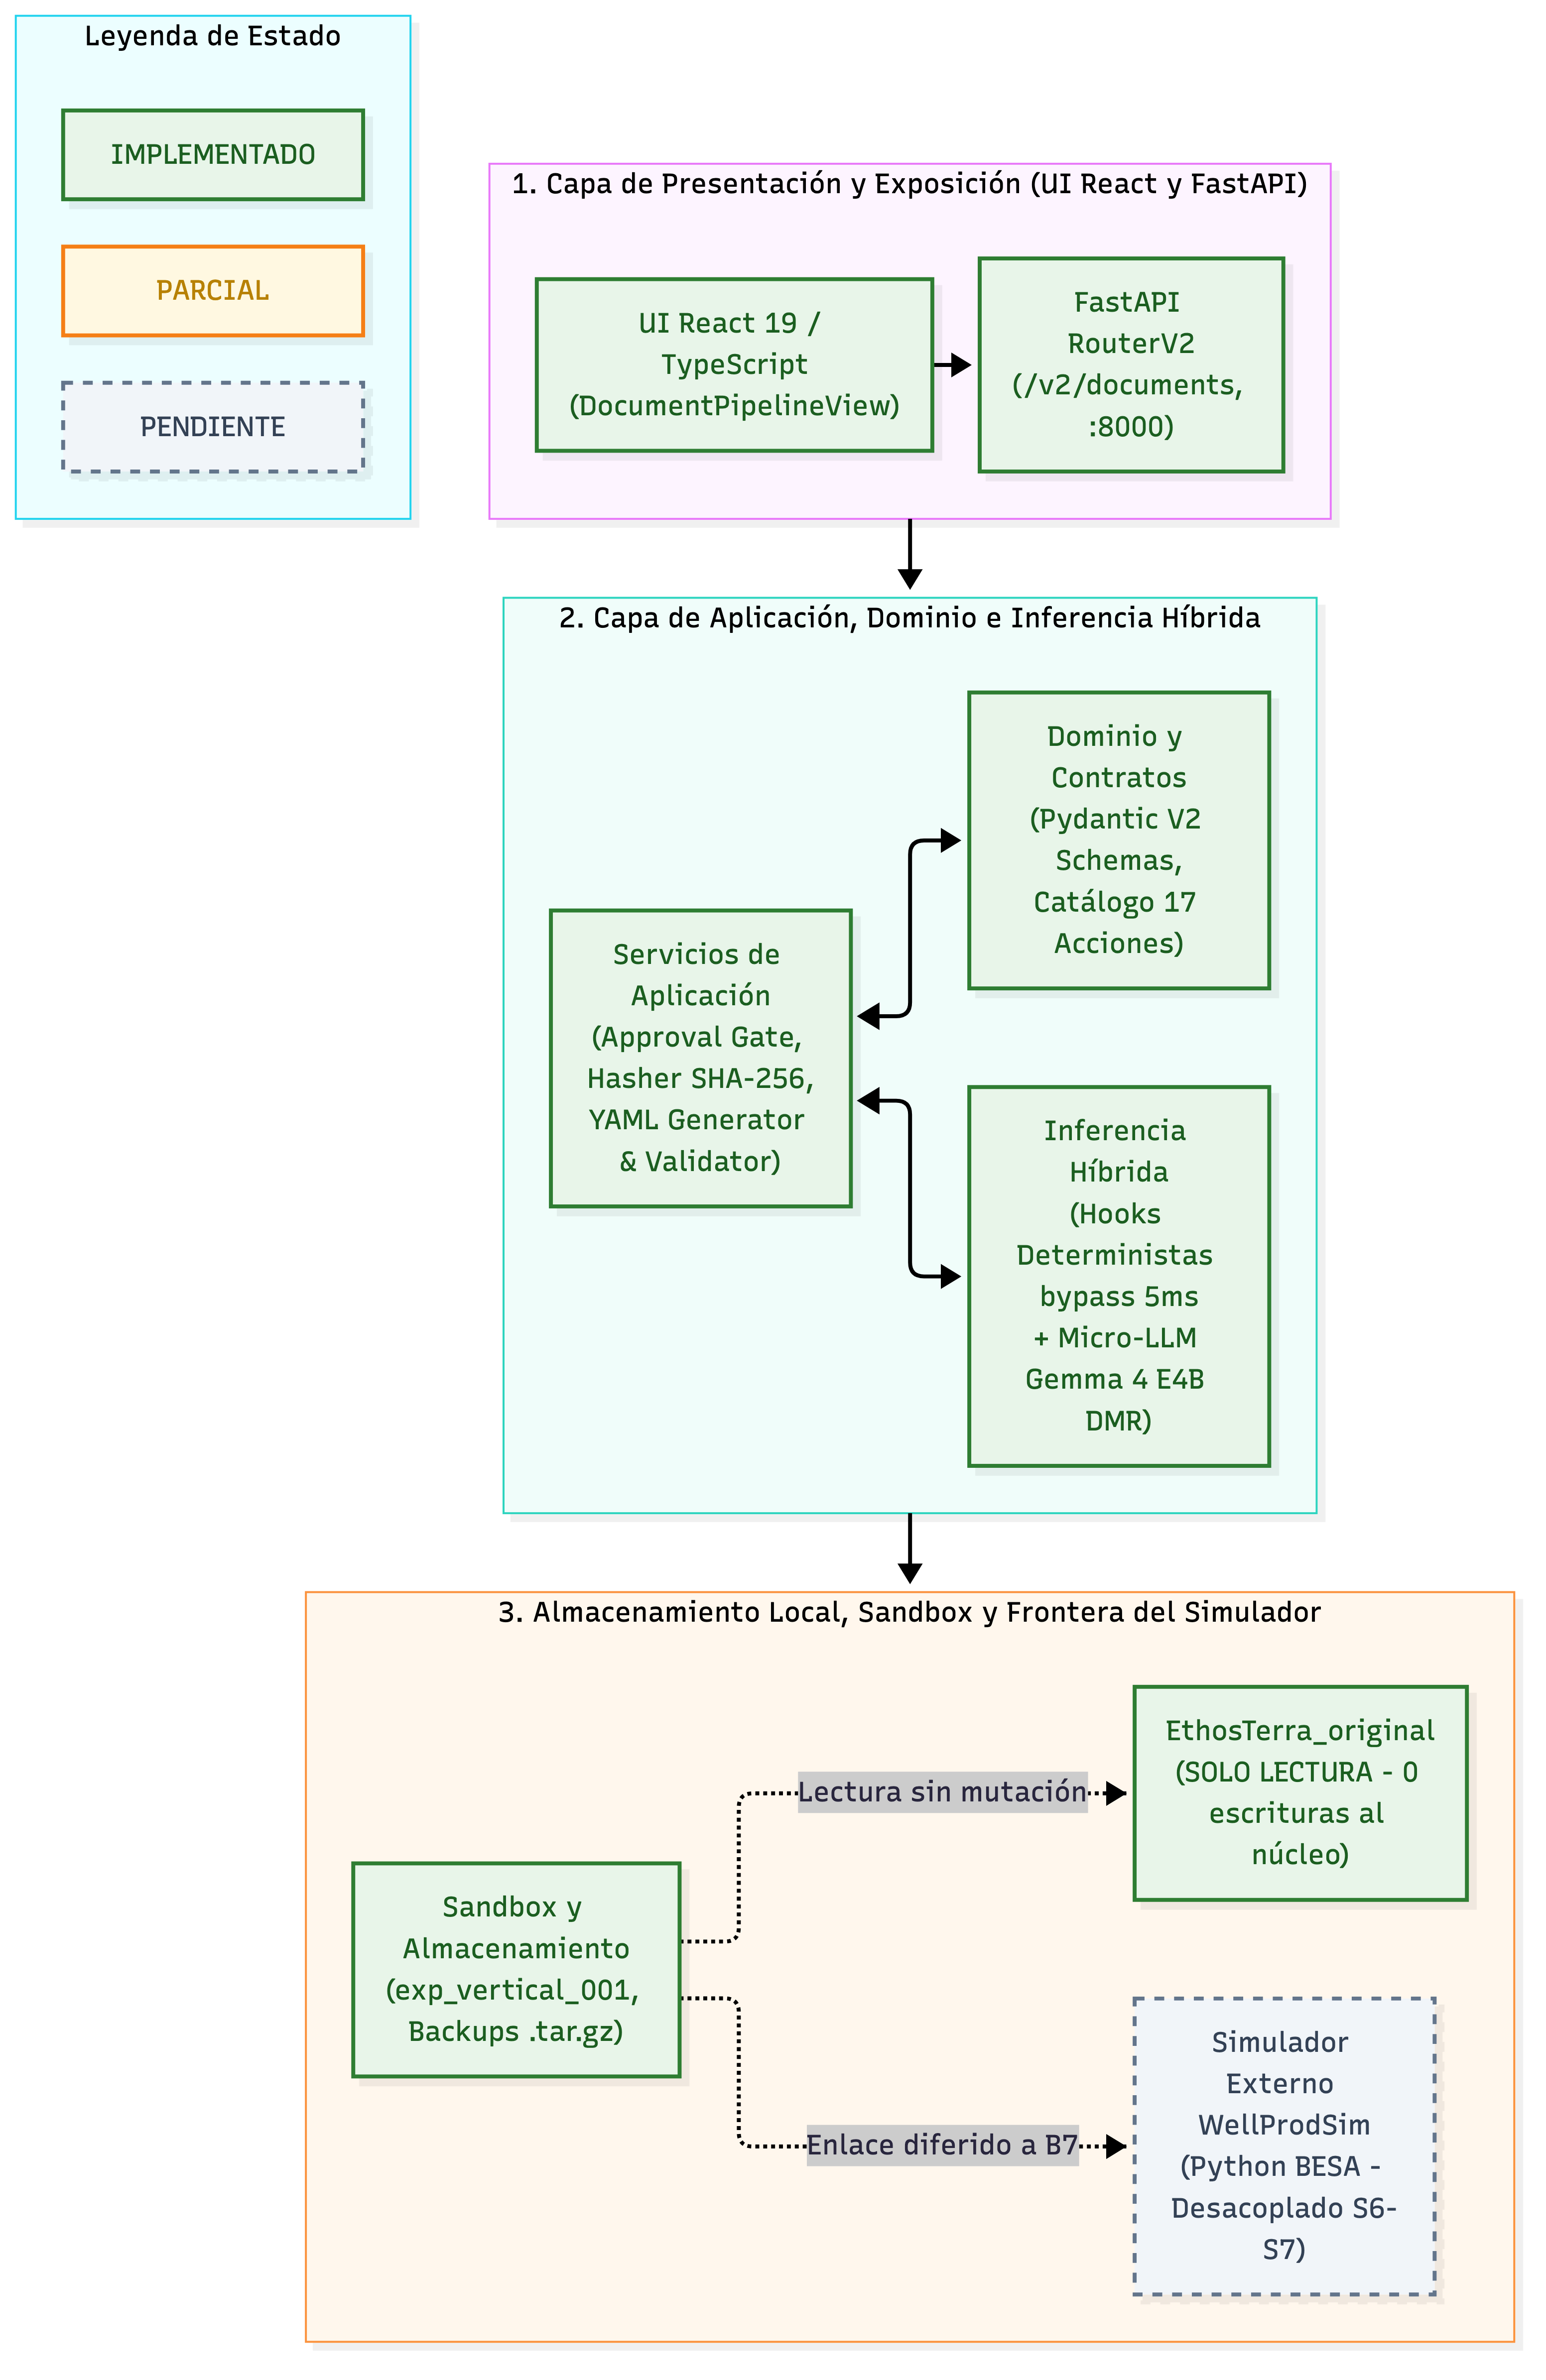
\includegraphics[width=0.88\textwidth,height=0.68\textheight,keepaspectratio]{docs/diagrams/out/d01_arch_layers_es.png}
    \caption{Figura D1. Arquitectura General por Capas del Sistema Híbrido eBDI. Detalla la interacción entre la interfaz React, la API FastAPI, los servicios de aplicación, el dominio, el runtime DMR local (offline-first), el sandbox de experimentación y la frontera desacoplada hacia el simulador.}
    \label{fig:d01_arch_layers_es}
\end{figure}

% --- Figura D4a: Flujo del Clasificador Híbrido (Parte 1: Ingesta, Normalización y Bypass Determinista) ---
\begin{figure}[htbp]
    \centering
    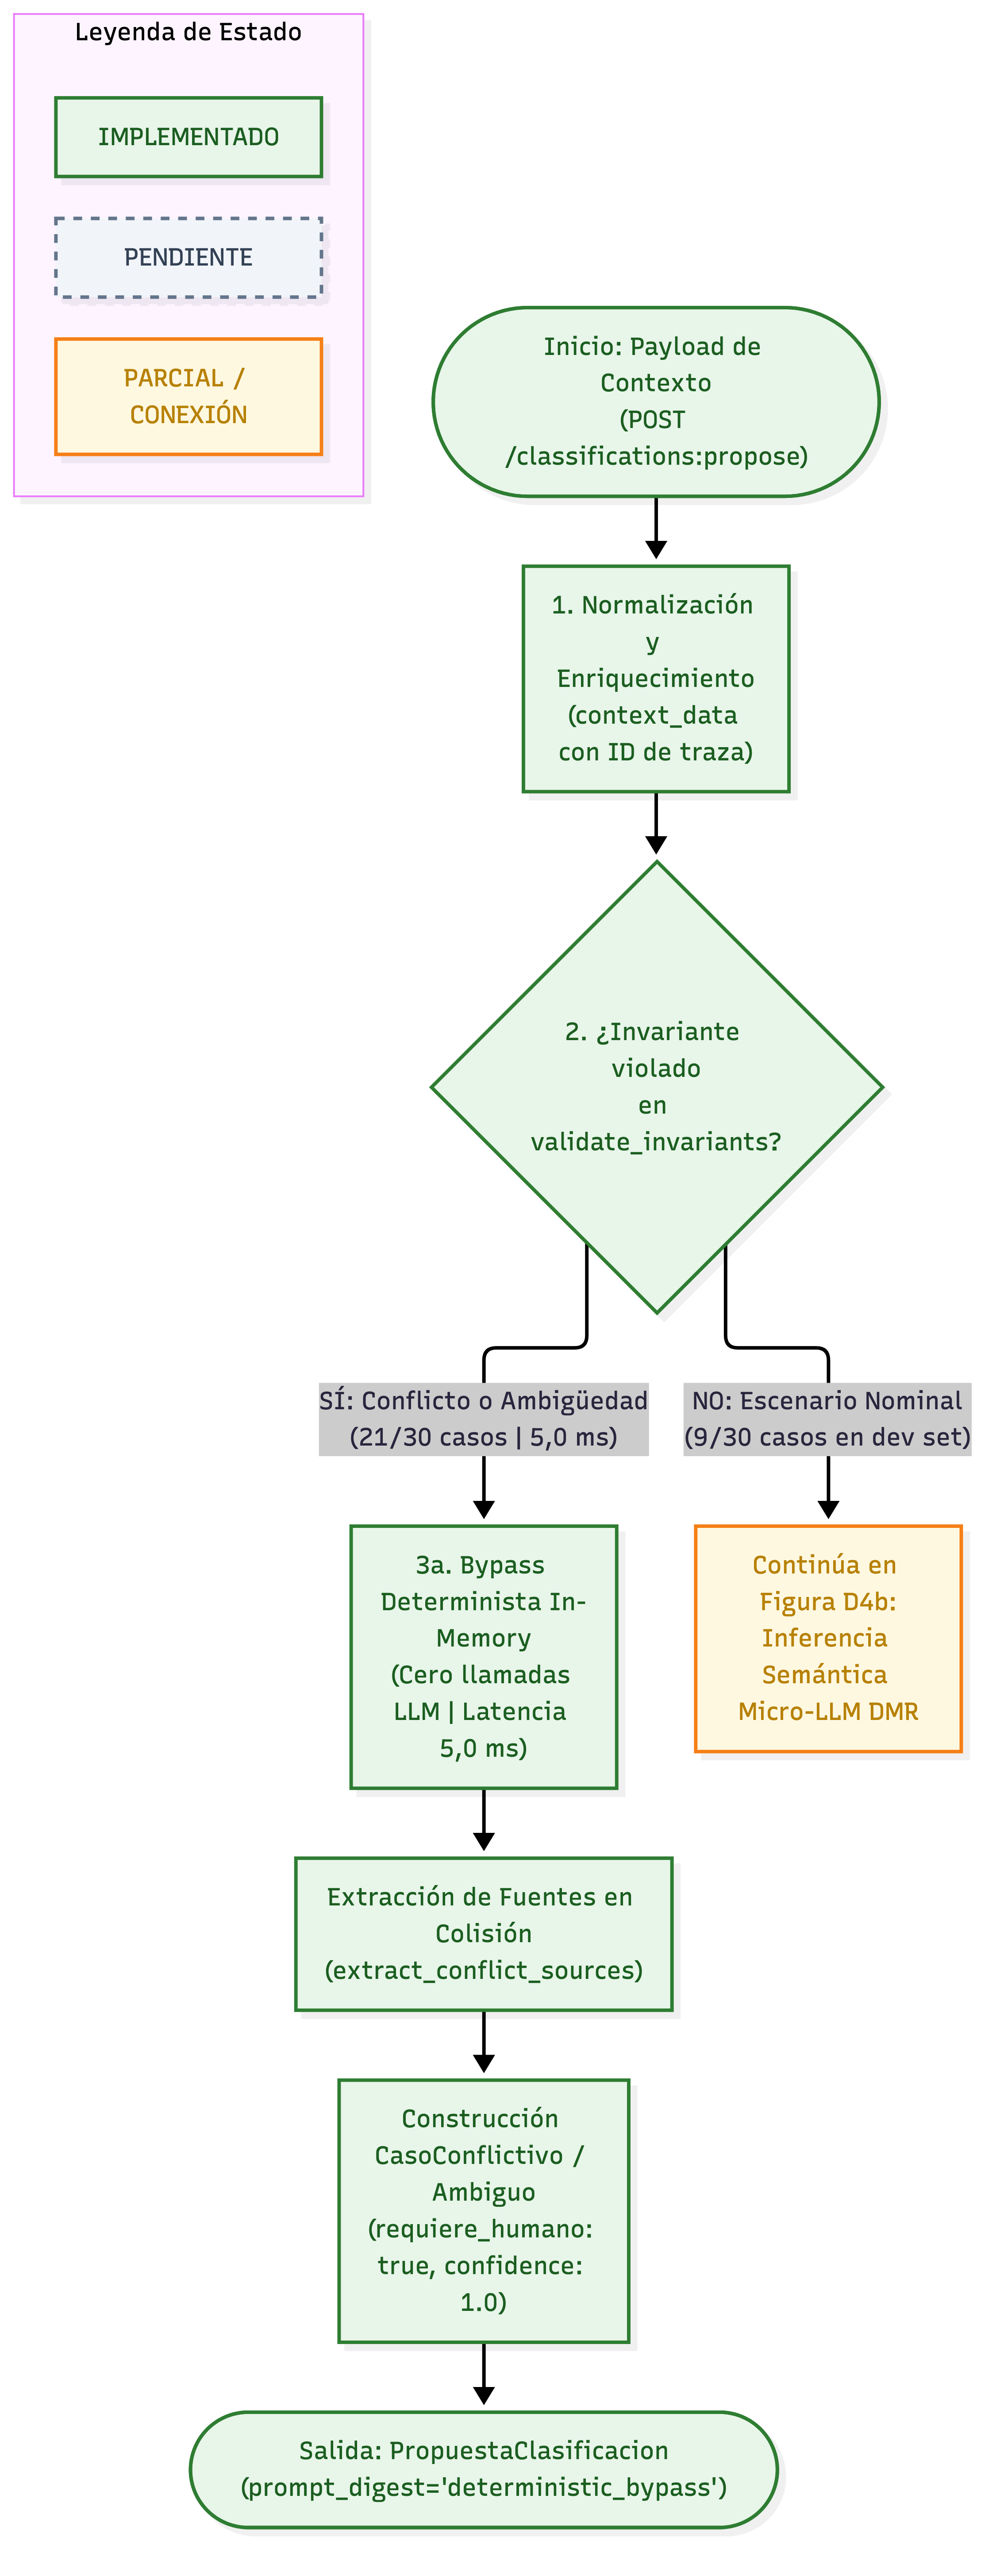
\includegraphics[width=0.88\textwidth,height=0.68\textheight,keepaspectratio]{docs/diagrams/out/d04a_classifier_flow_es.png}
    \caption{Figura D4a. Flujo del Clasificador Híbrido (Parte 1: Ingesta, Normalización y Bypass Determinista). Presenta la recepción de la solicitud declarativa, la normalización contextual y la evaluación de invariantes mediante hooks in-memory, resolviendo el 70\% de los casos del conjunto de desarrollo (21 de 30 casos) con latencia determinista de 5,0~ms sin invocar el modelo neuronal. Conecta con el punto A (Figura D4b).}
    \label{fig:d04a_classifier_flow_es}
\end{figure}

% --- Figura D4b: Flujo del Clasificador Híbrido (Parte 2: Inferencia Micro-LLM y Validación Pydantic V2) ---
\begin{figure}[htbp]
    \centering
    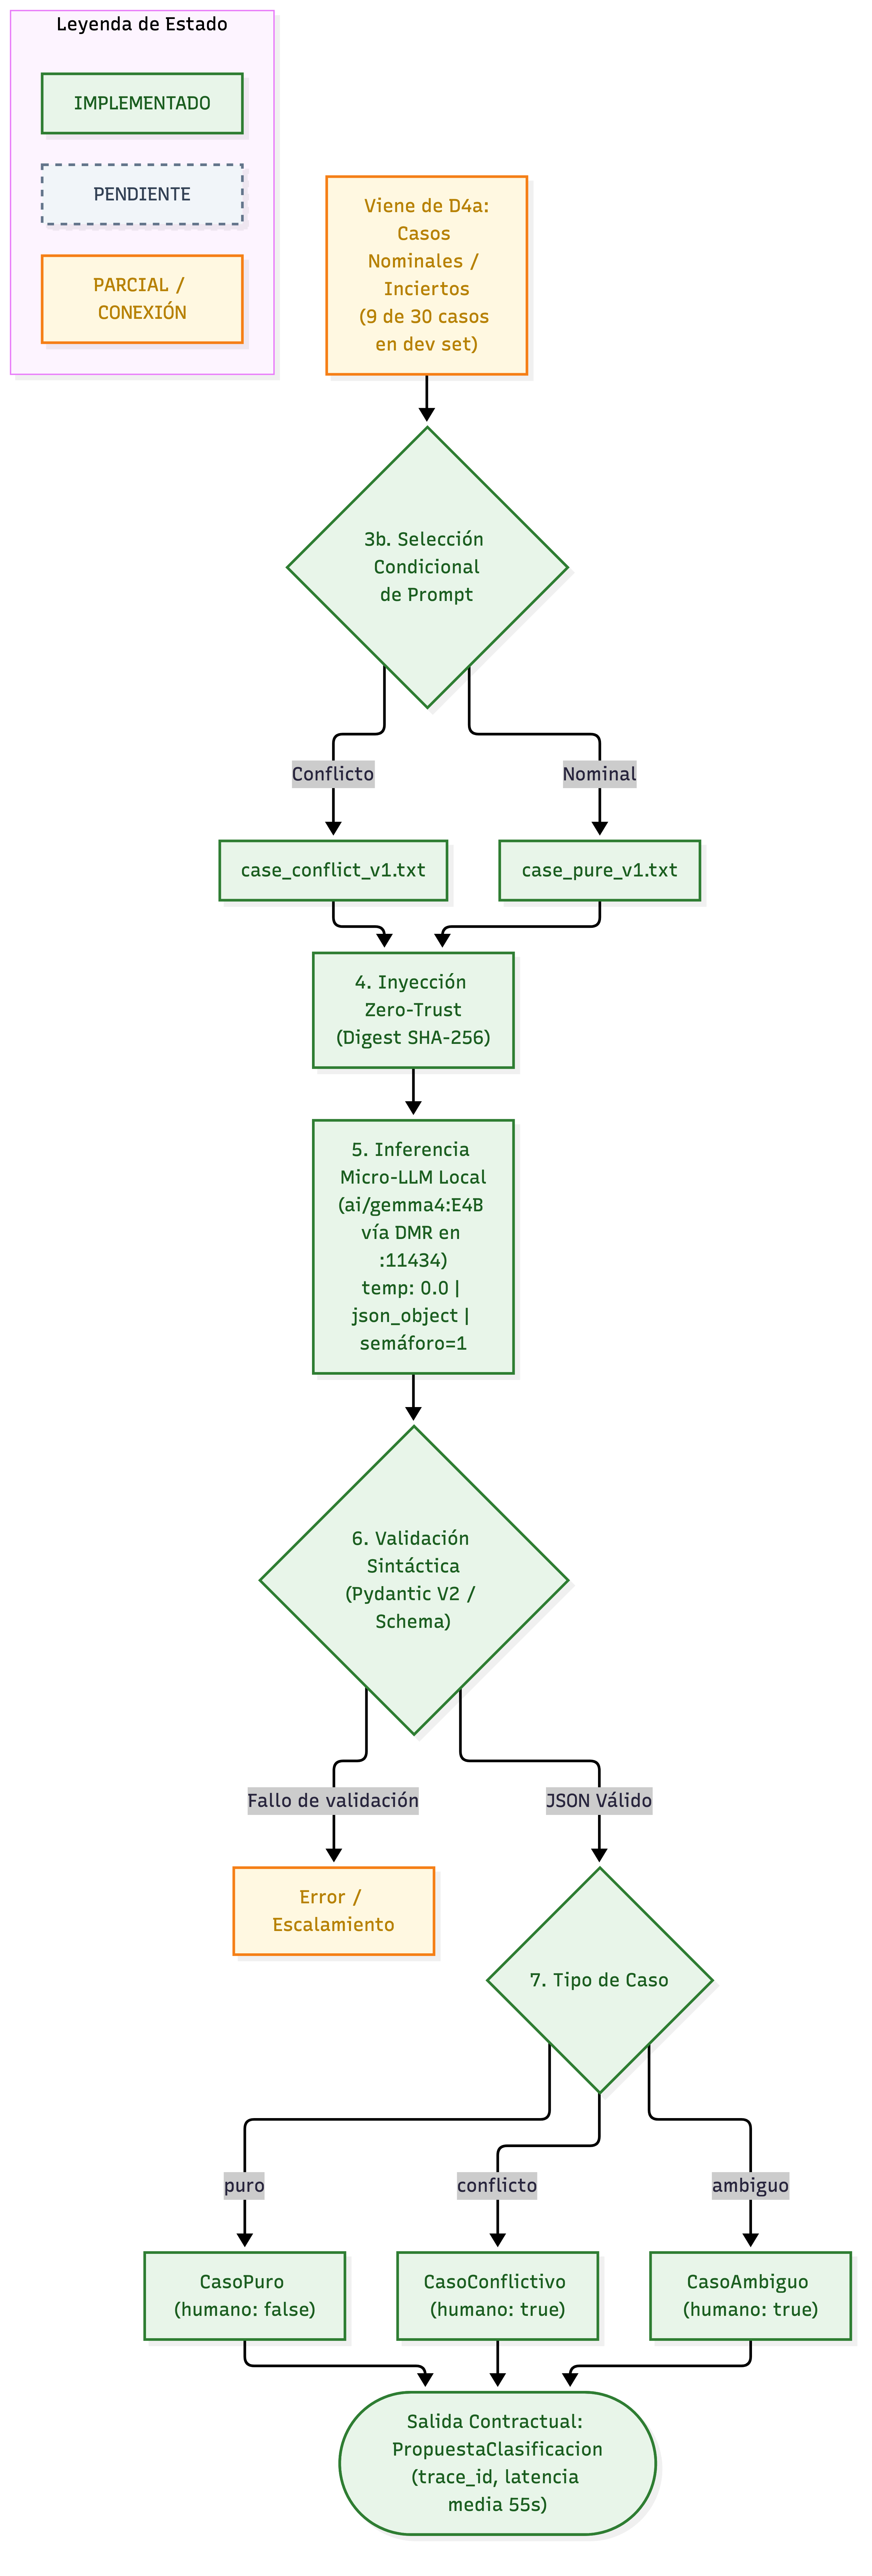
\includegraphics[width=0.88\textwidth,height=0.68\textheight,keepaspectratio]{docs/diagrams/out/d04b_classifier_flow_es.png}
    \caption{Figura D4b. Flujo del Clasificador Híbrido (Parte 2: Inferencia Micro-LLM y Validación Pydantic V2). Retoma desde el punto A (Figura D4a) ante casos complejos o ambiguos, ilustrando la selección condicional del prompt Zero-Trust, la inferencia local con \texttt{ai/gemma4:E4B} sobre Docker Model Runner (9 casos, latencia media 55.049,64~ms), el control sintáctico/semántico y la asignación final de intenciones o derivación a revisión humana.}
    \label{fig:d04b_classifier_flow_es}
\end{figure}

% --- Figura D6a: Flujo de Estados del Documento (Parte 1: Borrador a Analizado, Estructuración y Rutas de Bloqueo) ---
\begin{figure}[htbp]
    \centering
    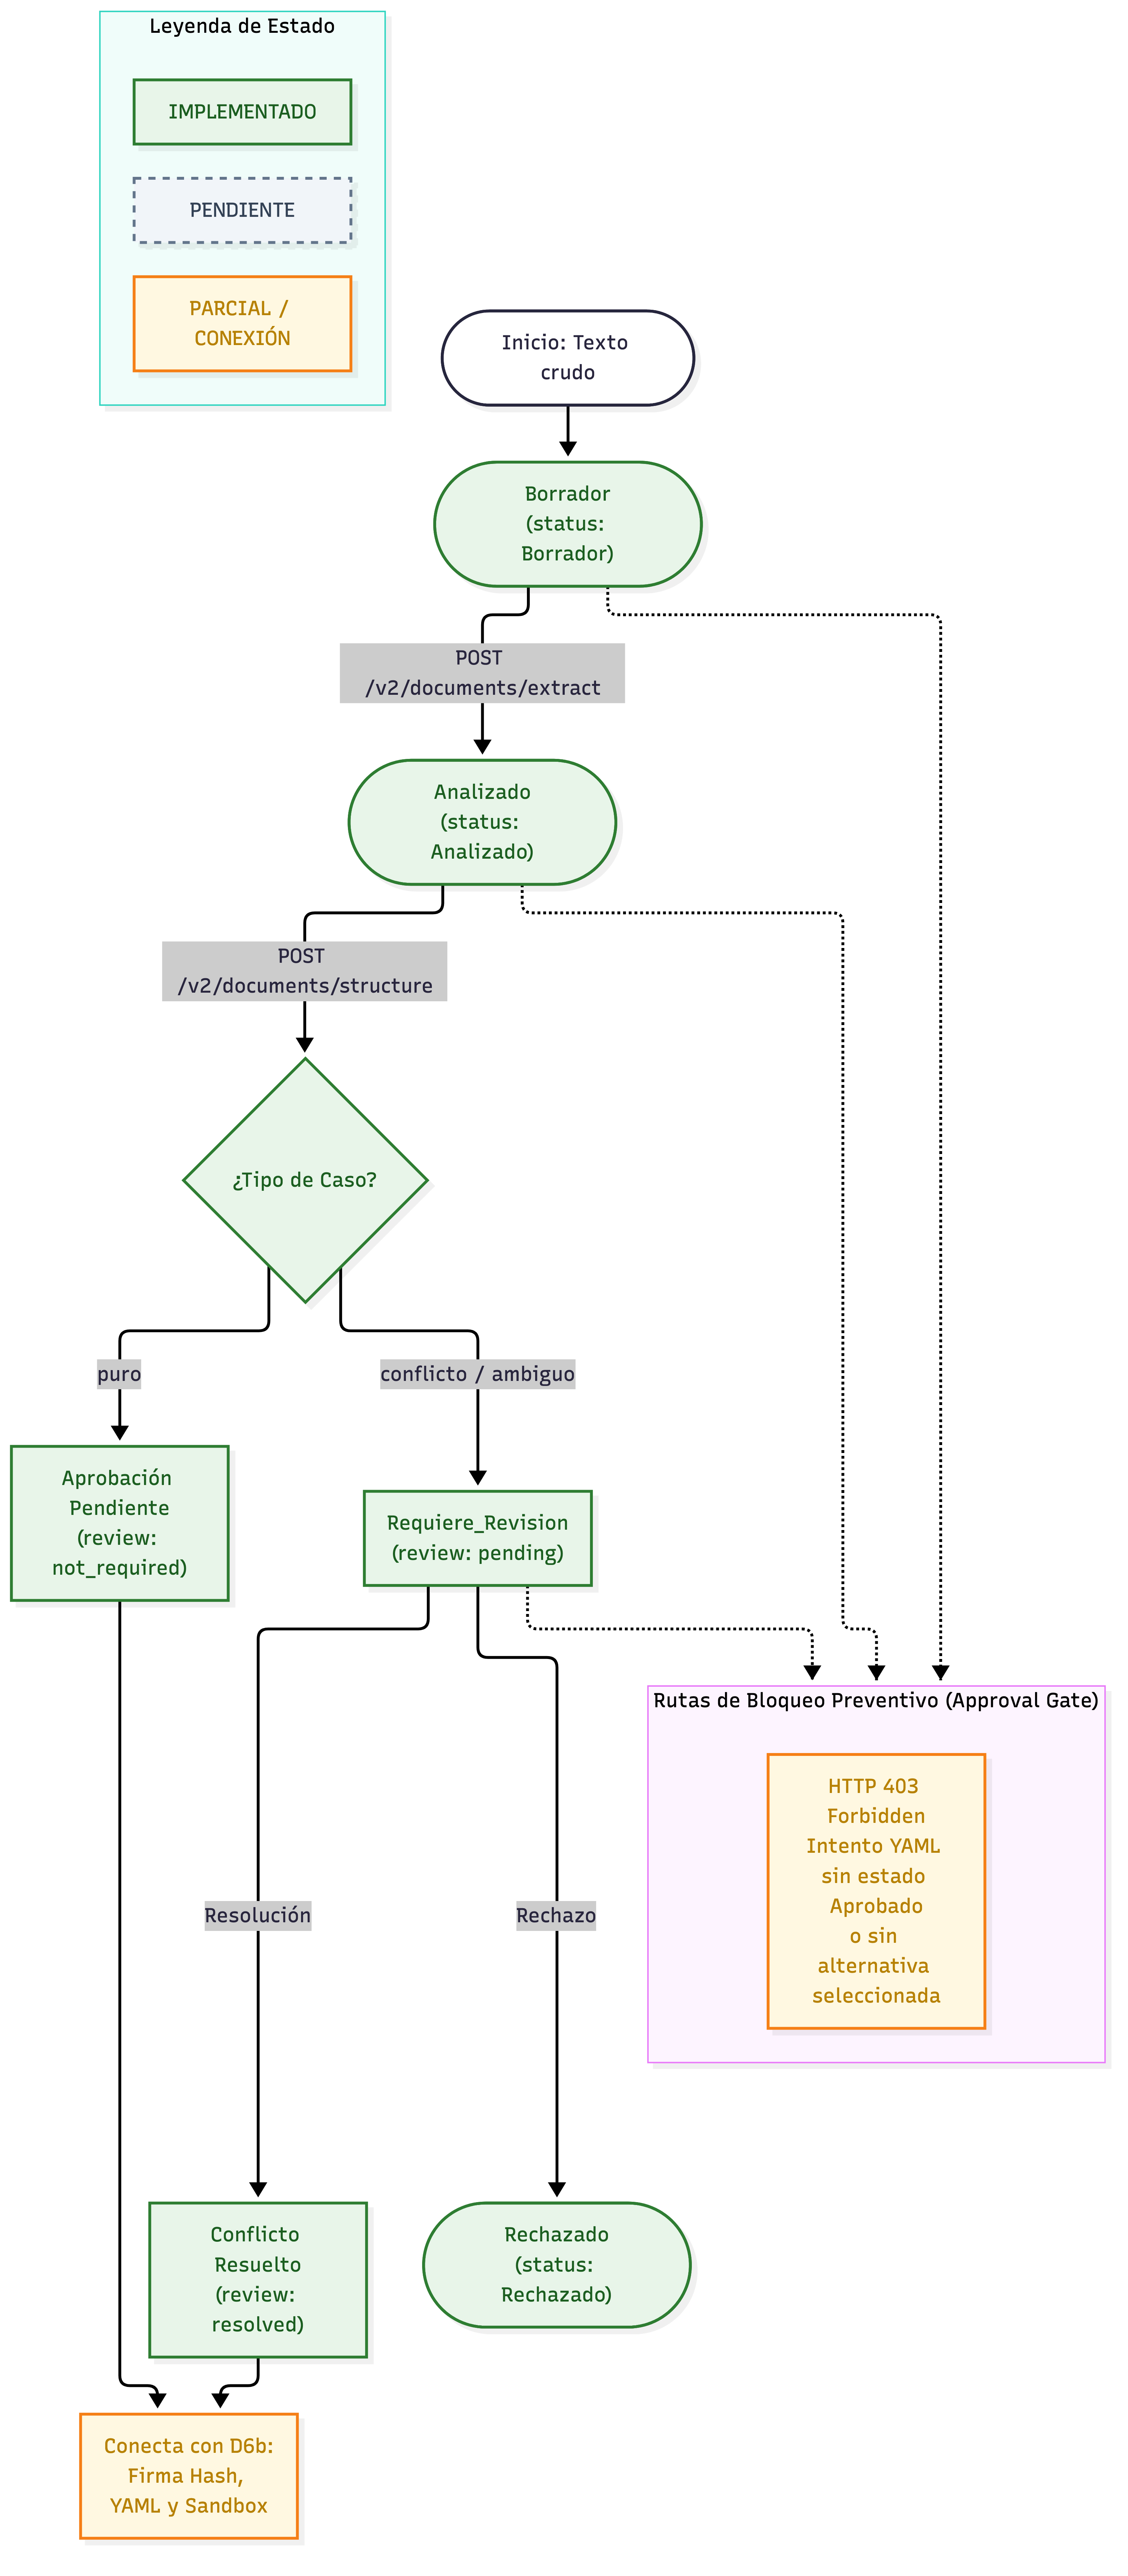
\includegraphics[width=0.88\textwidth,height=0.68\textheight,keepaspectratio]{docs/diagrams/out/d06a_document_lifecycle_es.png}
    \caption{Figura D6a. Flujo de Estados del Documento Operativo (Parte 1: Borrador a Analizado, Estructuración y Rutas de Bloqueo). Modela el ciclo de vida inicial del documento desde su creación en estado \texttt{Borrador}, el análisis estructurado (\texttt{GoalSpecArtifact}, \texttt{PlanSpecArtifact}) y la bifurcación hacia \texttt{Requiere\_Revision}, \texttt{Rechazado} o \texttt{Analizado}. Representa las compuertas de seguridad que impiden avanzar con esquemas inválidos o intenciones contradictorias. Conecta con el punto de control Aprobación (Figura D6b).}
    \label{fig:d06a_document_lifecycle_es}
\end{figure}

% --- Figura D6b: Flujo de Estados del Documento (Parte 2: Aprobación, Hash Canónico e Instalación en Sandbox) ---
\begin{figure}[htbp]
    \centering
    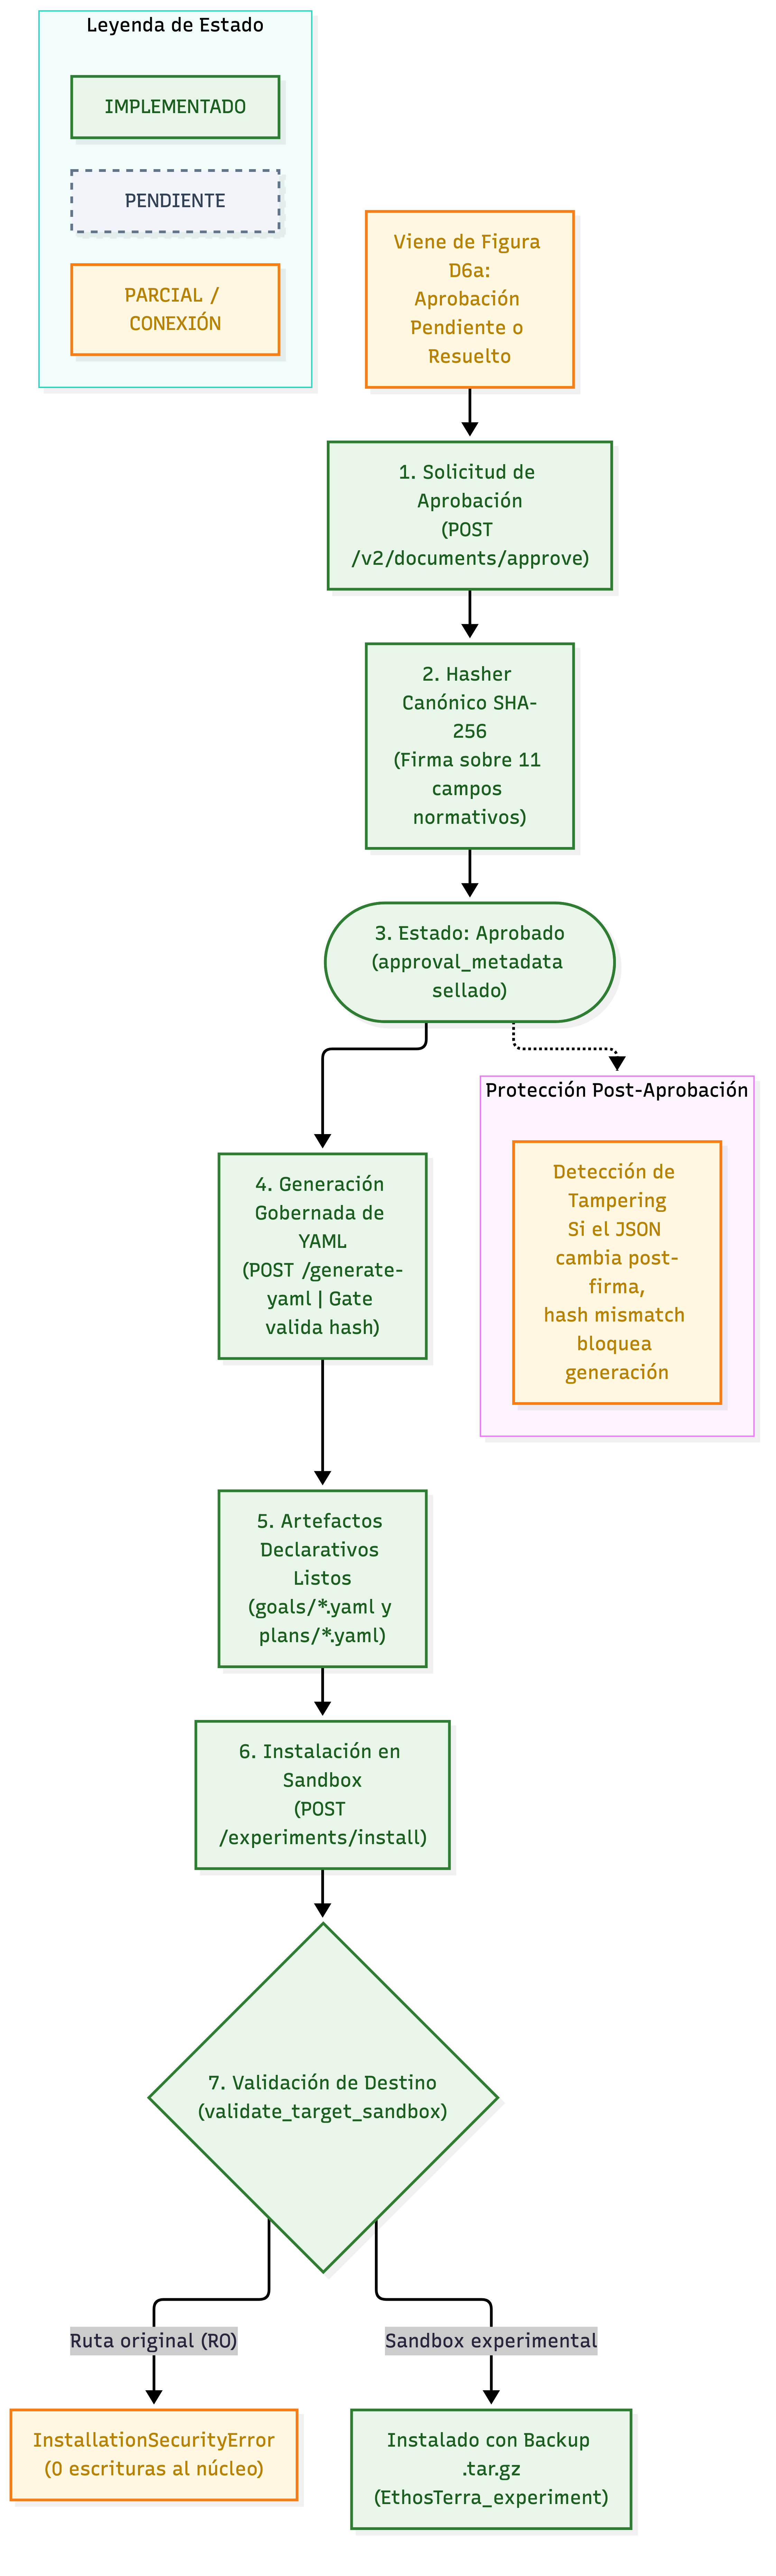
\includegraphics[width=0.88\textwidth,height=0.68\textheight,keepaspectratio]{docs/diagrams/out/d06b_document_lifecycle_es.png}
    \caption{Figura D6b. Flujo de Estados del Documento Operativo (Parte 2: Aprobación, Hash Canónico e Instalación en Sandbox). Retoma desde el estado \texttt{Analizado} (Figura D6a) y detalla la transición a \texttt{Aprobado} mediante firma humana con hash canónico SHA-256 de 11 campos, la generación de YAML confinado, la instalación con respaldo comprimido (.tar.gz) y el bloqueo inmediato con HTTP 403 o rollback atómico ante alteración posterior (tampering).}
    \label{fig:d06b_document_lifecycle_es}
\end{figure}

% --- Figura D11: Mapa de Estado y Hoja de Ruta de Desarrollo ---
\begin{figure}[htbp]
    \centering
    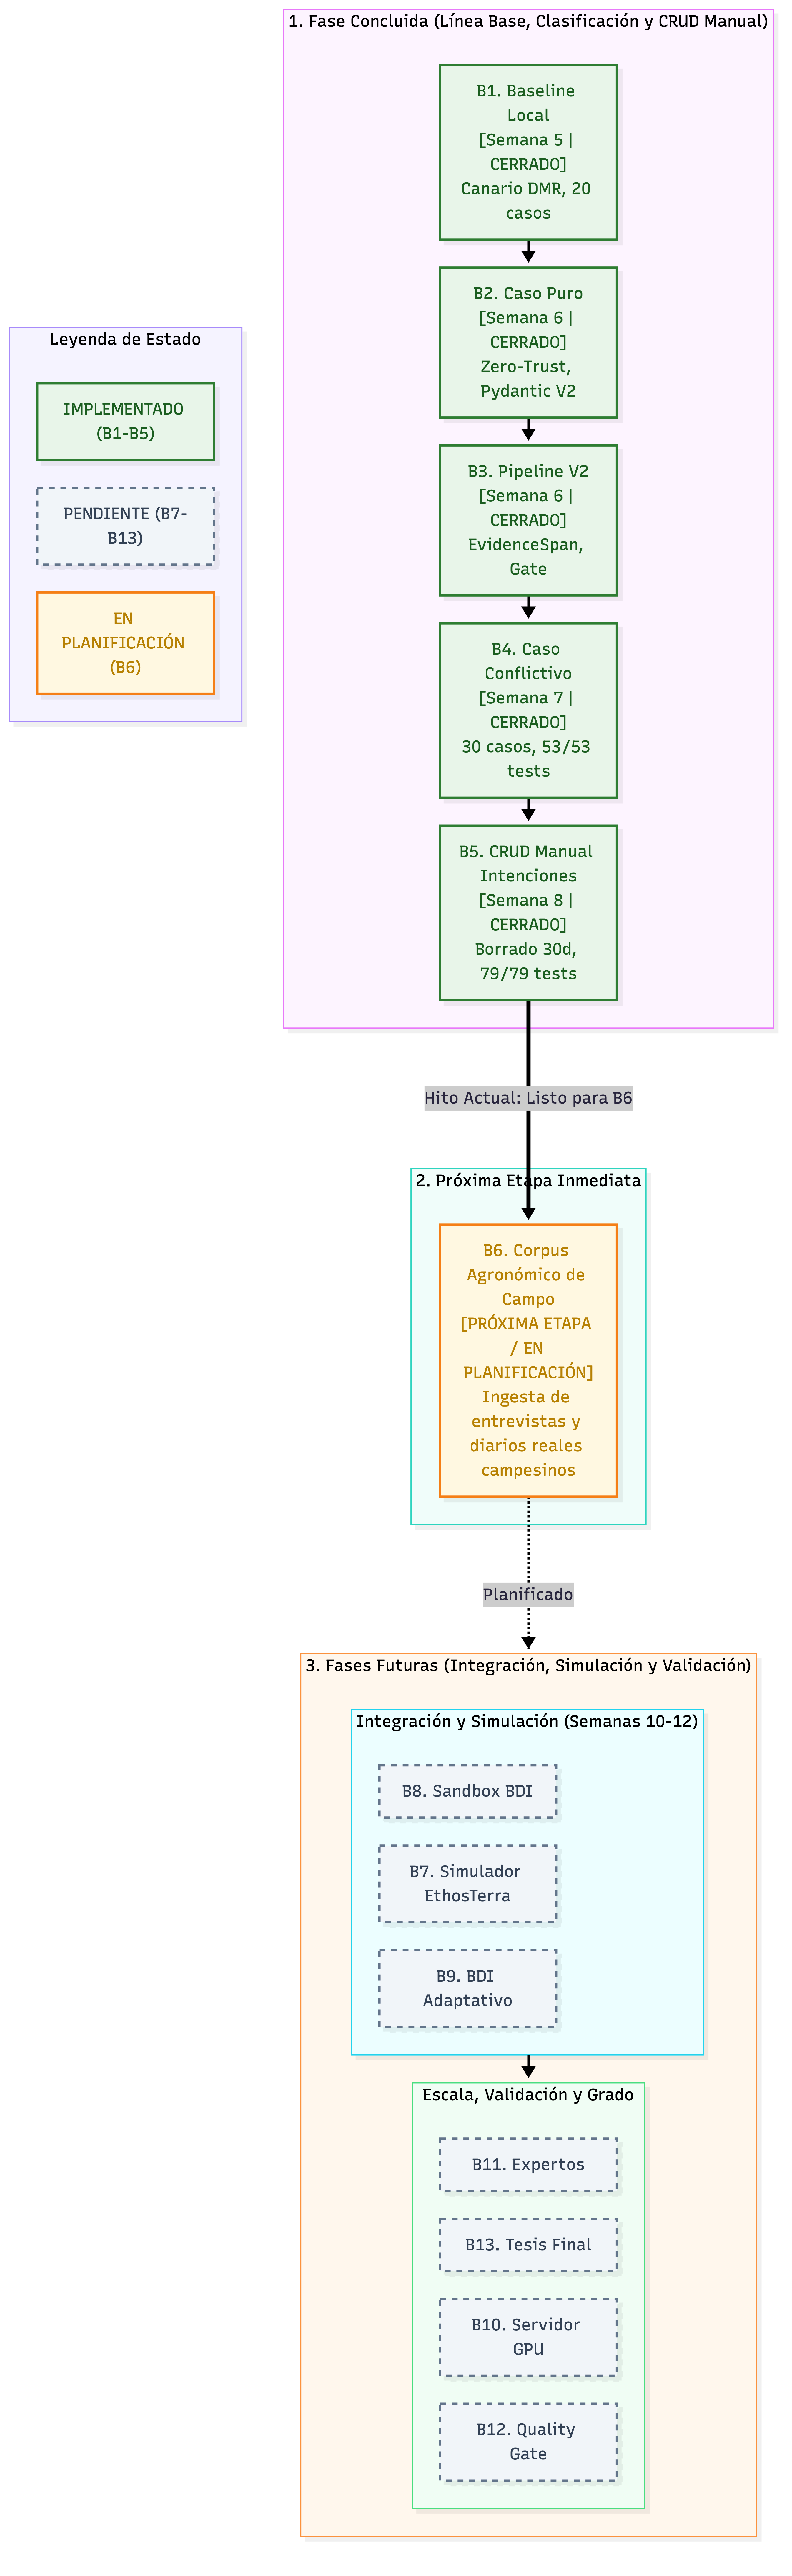
\includegraphics[width=0.88\textwidth,height=0.68\textheight,keepaspectratio]{docs/diagrams/out/d11_status_roadmap_es.png}
    \caption{Figura D11. Mapa de Estado y Hoja de Ruta de Desarrollo (Bloques B1 a B13). Visualiza el progreso consolidado de los bloques concluidos (B1--B5, con 79/79 pruebas aprobadas), la posición del próximo incremento (B6: Corpus agronómico de campo) y la planificación de las fases subsiguientes de integración y validación (B7--B13).}
    \label{fig:d11_status_roadmap_es}
\end{figure}


\clearpage

% ==============================================================================
% PARTE II: FIGURAS EN ESPAÑOL — ANEXO METODOLÓGICO Y TÉCNICO
% ==============================================================================

% --- Figura D2: Contexto del Sistema (C4 Nivel 1) ---
\begin{figure}[htbp]
    \centering
    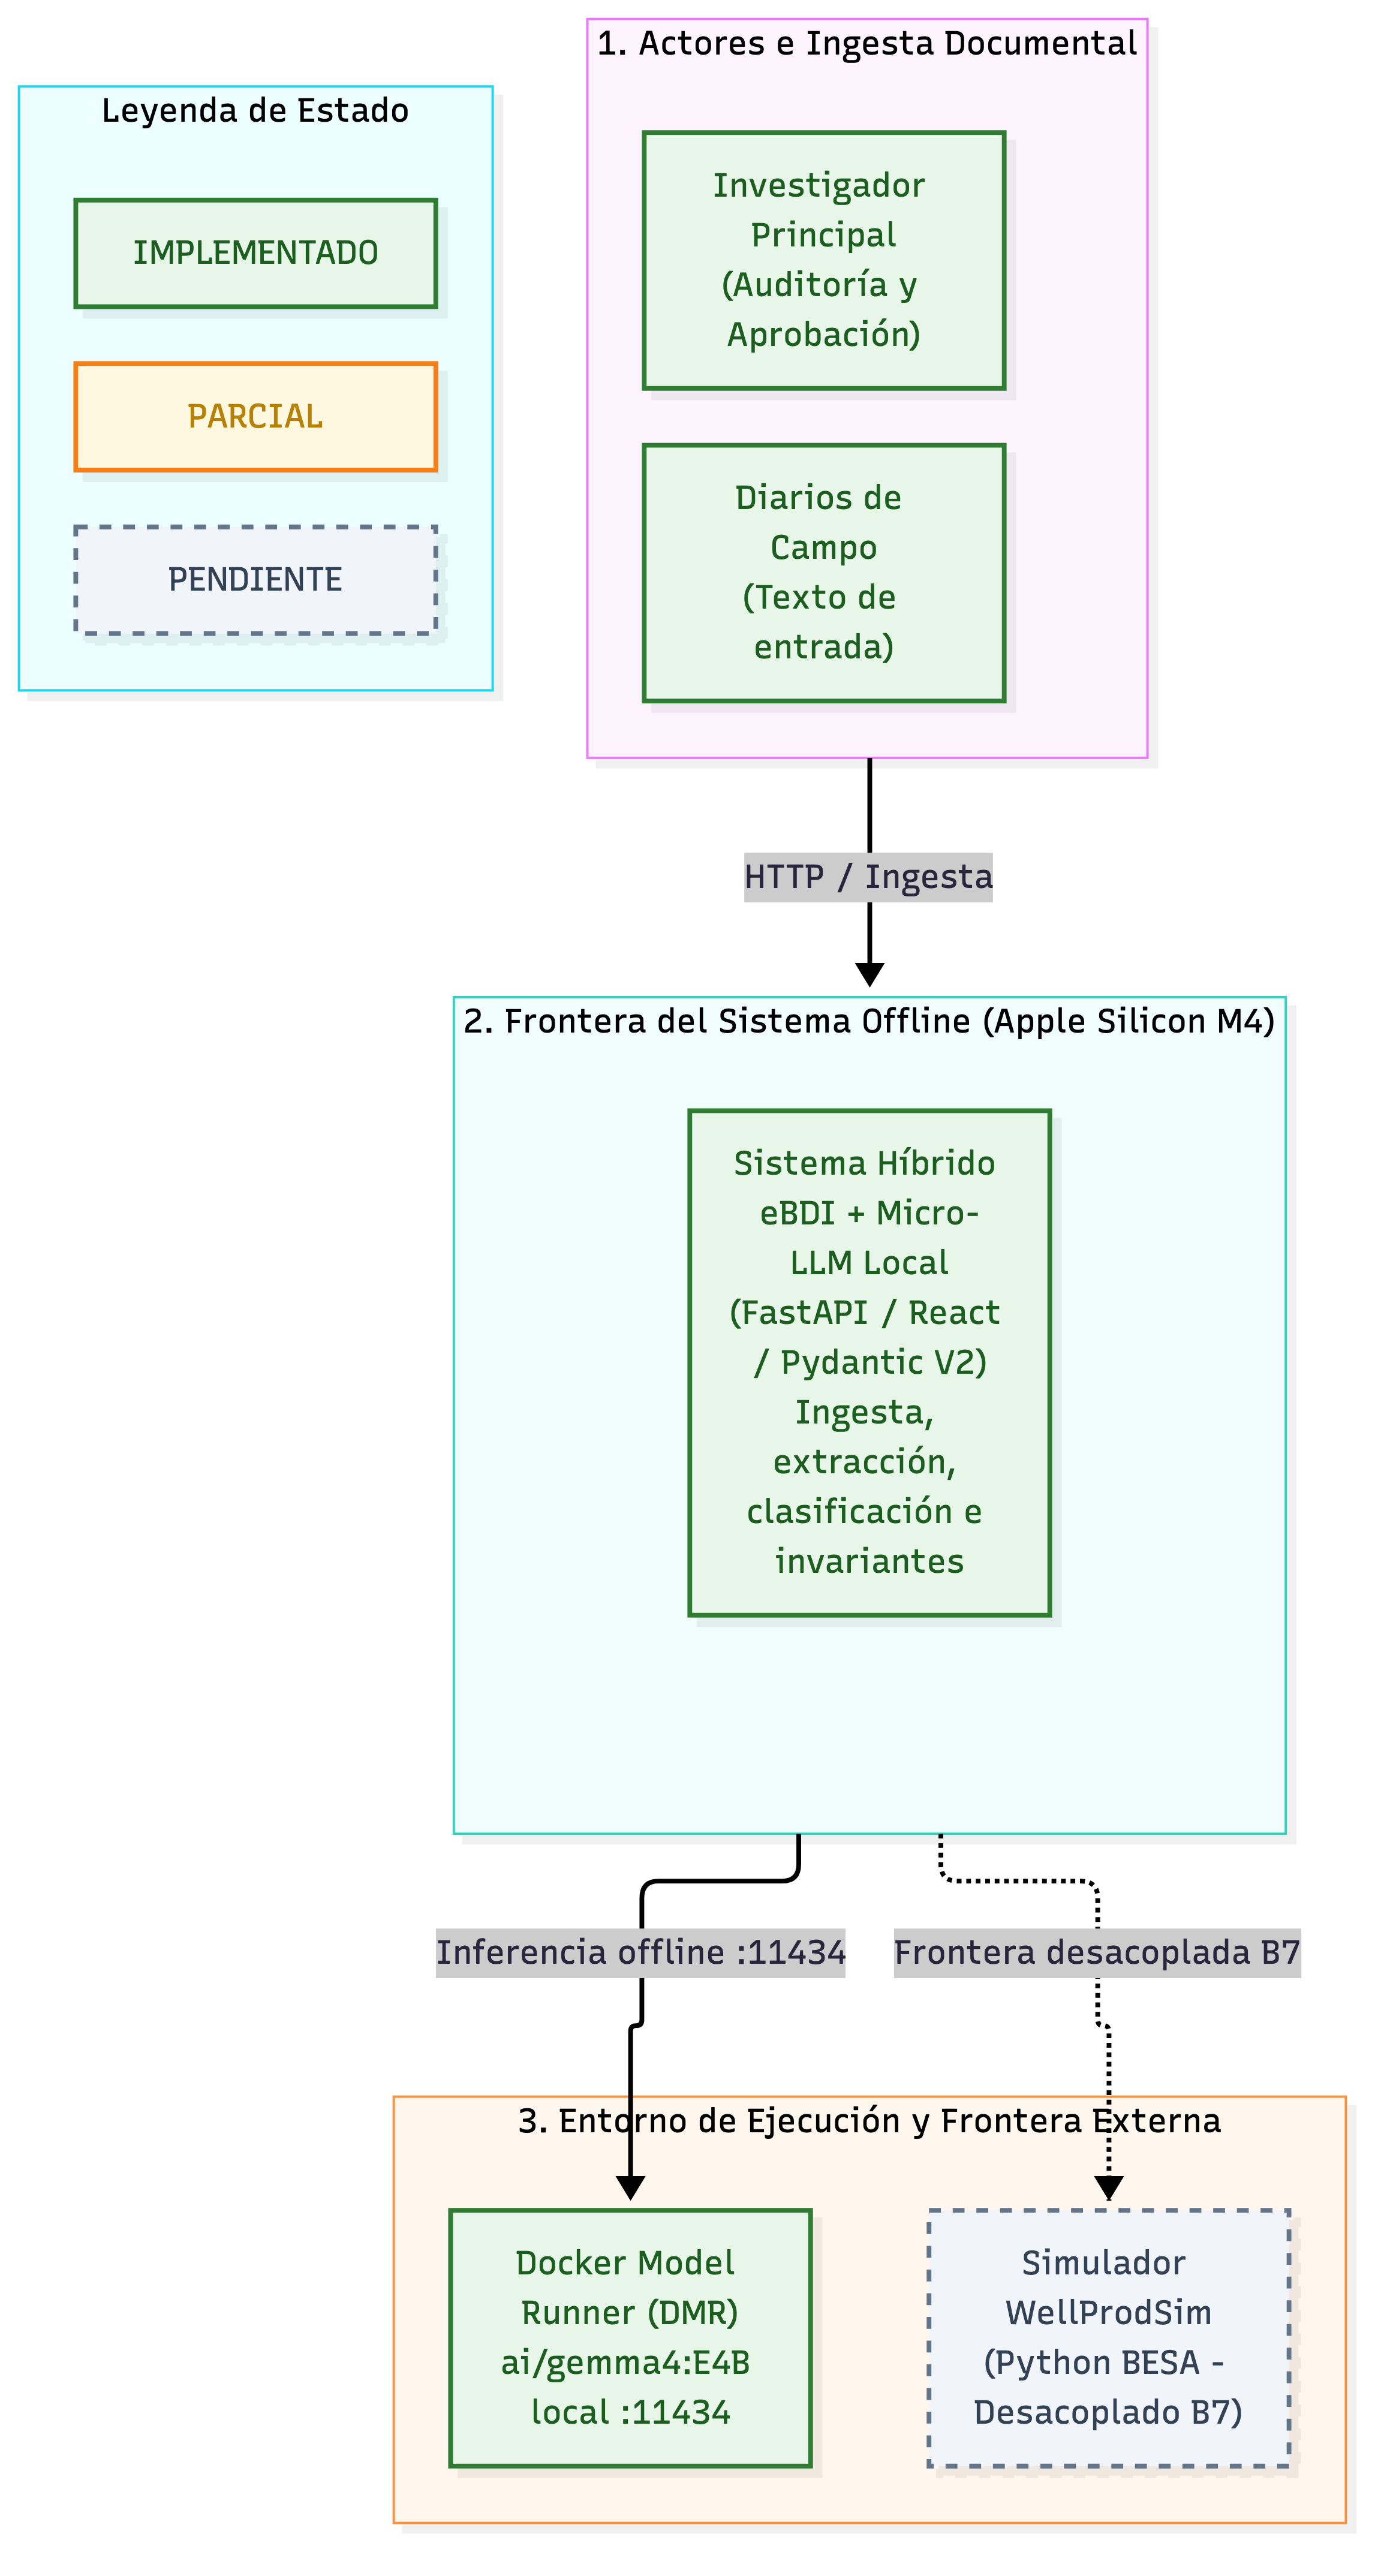
\includegraphics[width=0.88\textwidth,height=0.68\textheight,keepaspectratio]{docs/diagrams/out/d02_c4_context_es.png}
    \caption{Figura D2. Diagrama de Contexto del Sistema (C4 Nivel 1). Delimita los actores humanos (investigador principal y directores evaluadores), las fuentes documentales de campo, el runtime de inferencia Docker Model Runner y la frontera de ejecución 100\% offline en hardware Apple Silicon M4.}
    \label{fig:d02_c4_context_es}
\end{figure}

% --- Figura D3: Componentes del Backend (C4 Nivel 3) ---
\begin{figure}[htbp]
    \centering
    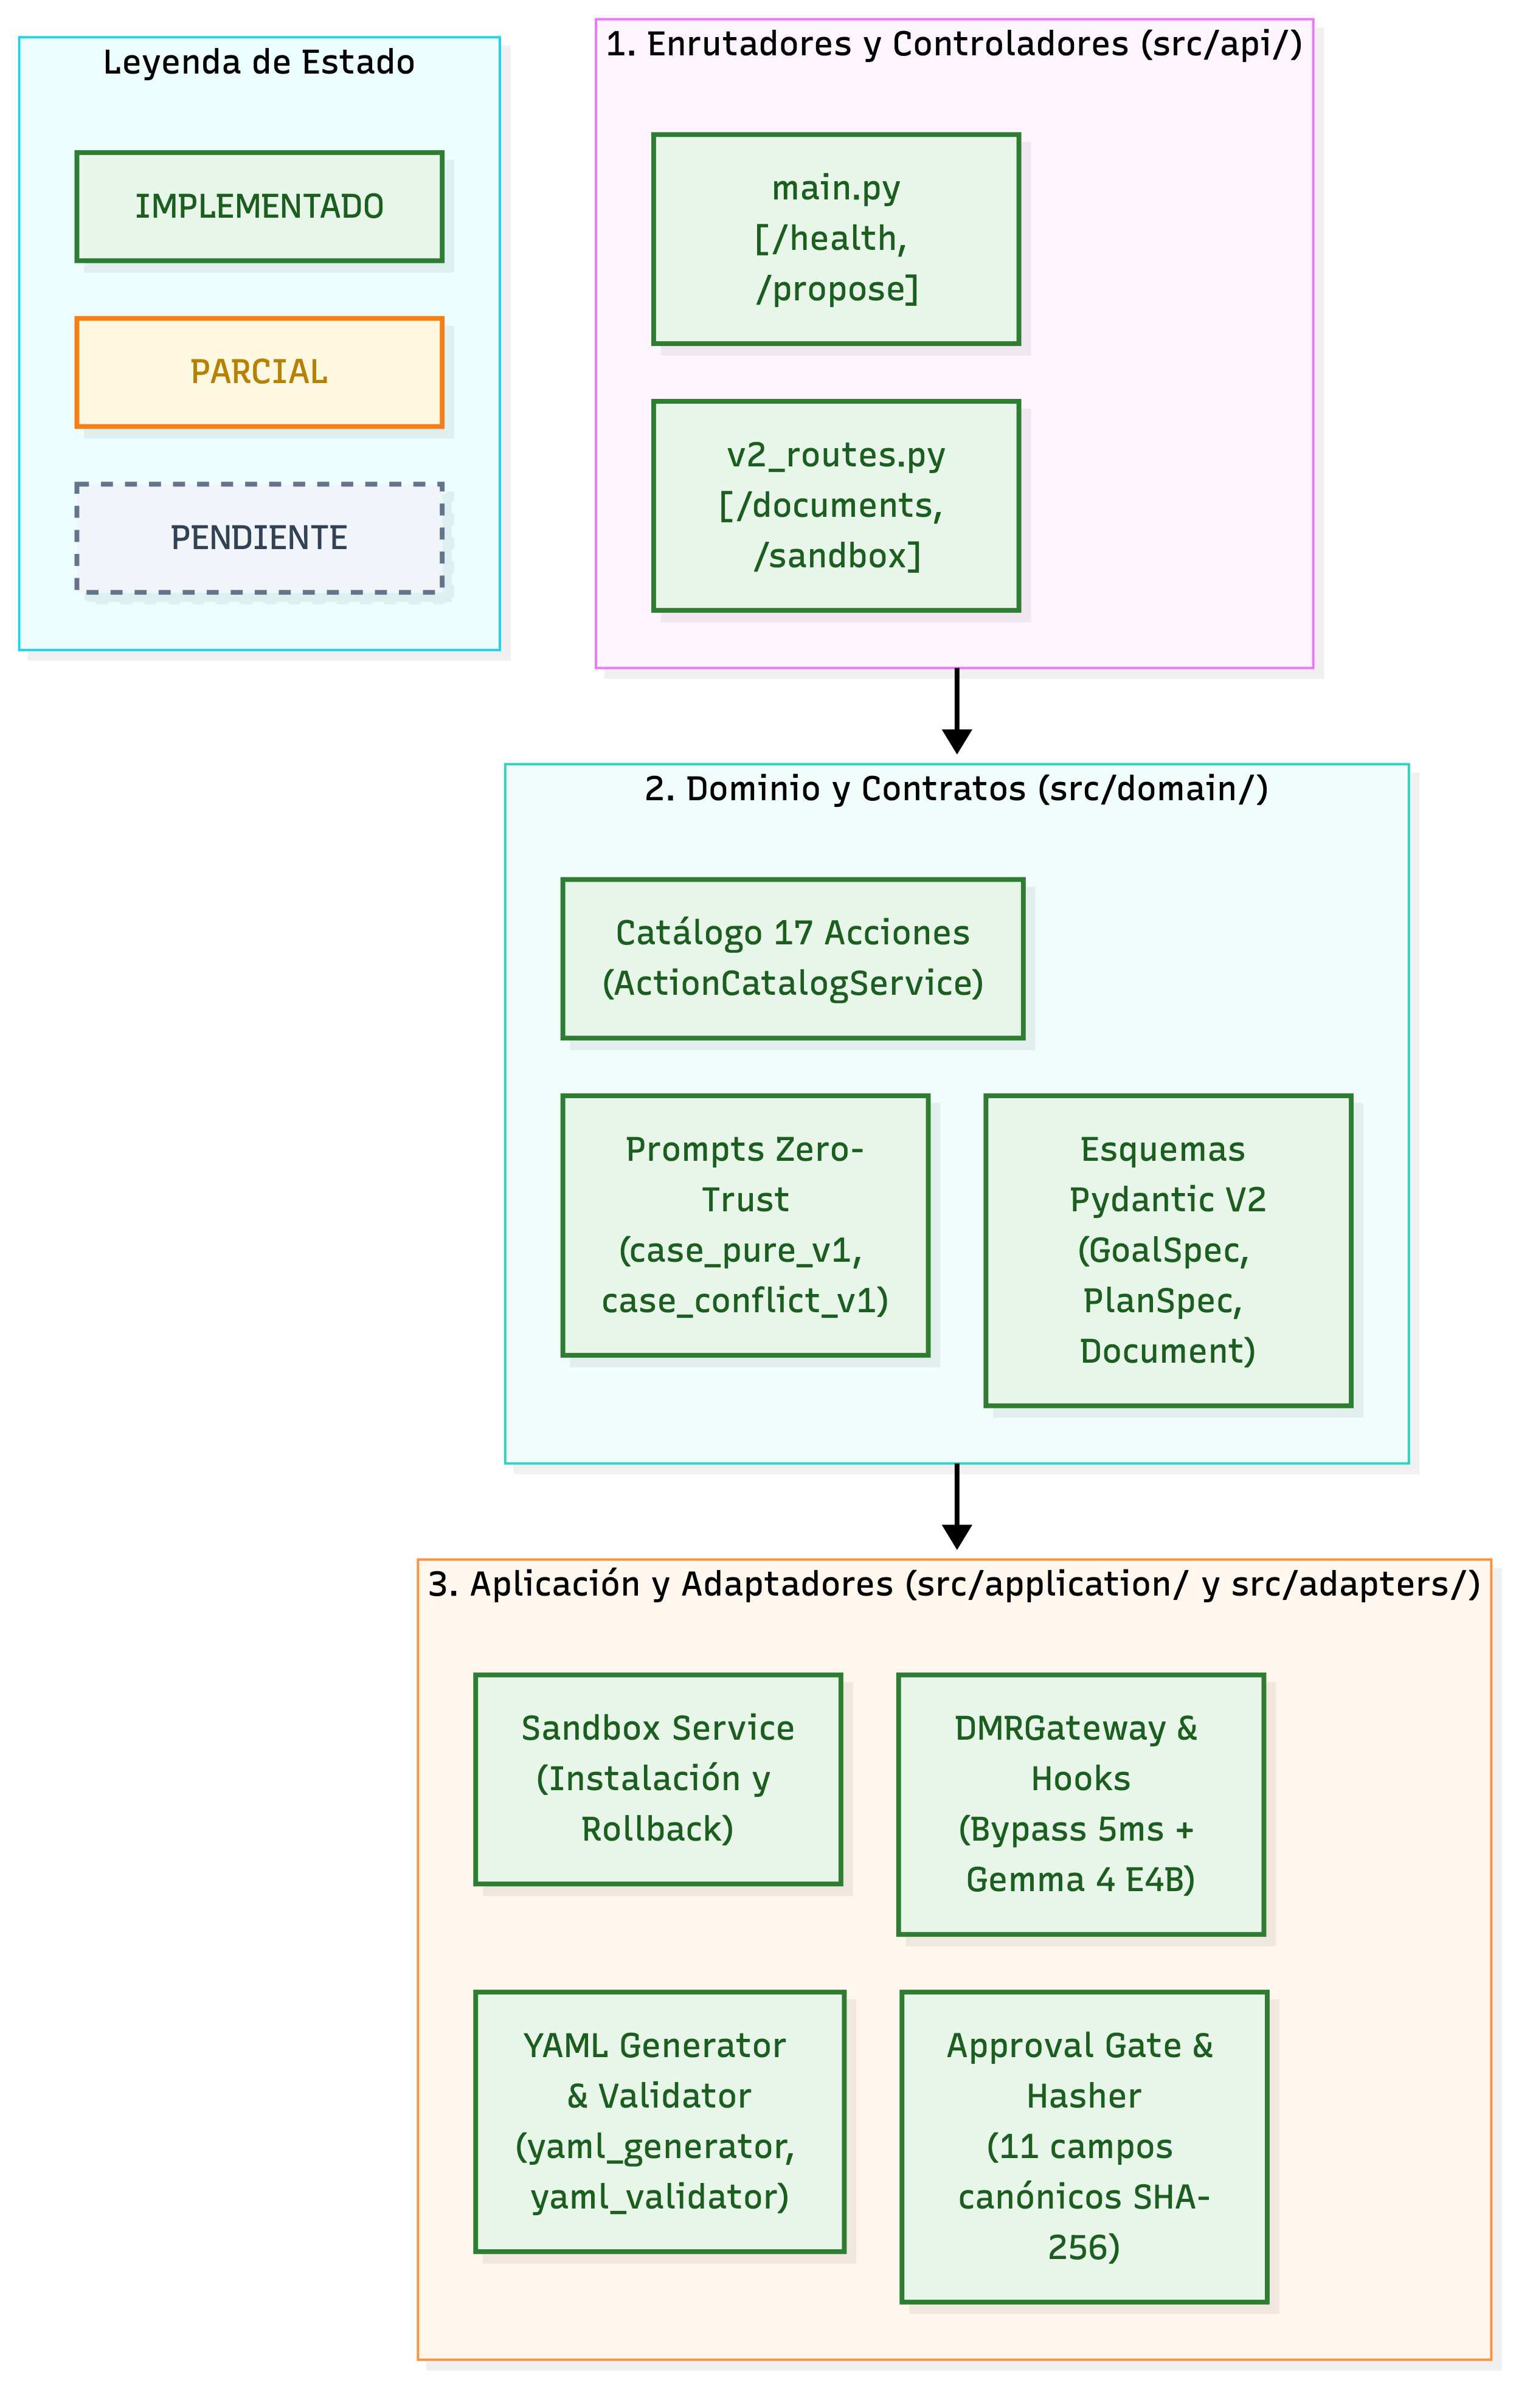
\includegraphics[width=0.88\textwidth,height=0.68\textheight,keepaspectratio]{docs/diagrams/out/d03_c4_components_es.png}
    \caption{Figura D3. Componentes Internos del Backend (C4 Nivel 3). Especifica la organización modular en \texttt{apps/api/src/}: enrutadores, esquemas Pydantic V2, catálogo verificado de 17 acciones de EthosTerra, hasher canónico SHA-256 de 11 campos y servicios de sandbox.}
    \label{fig:d03_c4_components_es}
\end{figure}

% --- Figura D5a: Flujo del Caso Conflictivo (Parte 1: Detección de Colisión y Trazabilidad de Fuentes) ---
\begin{figure}[htbp]
    \centering
    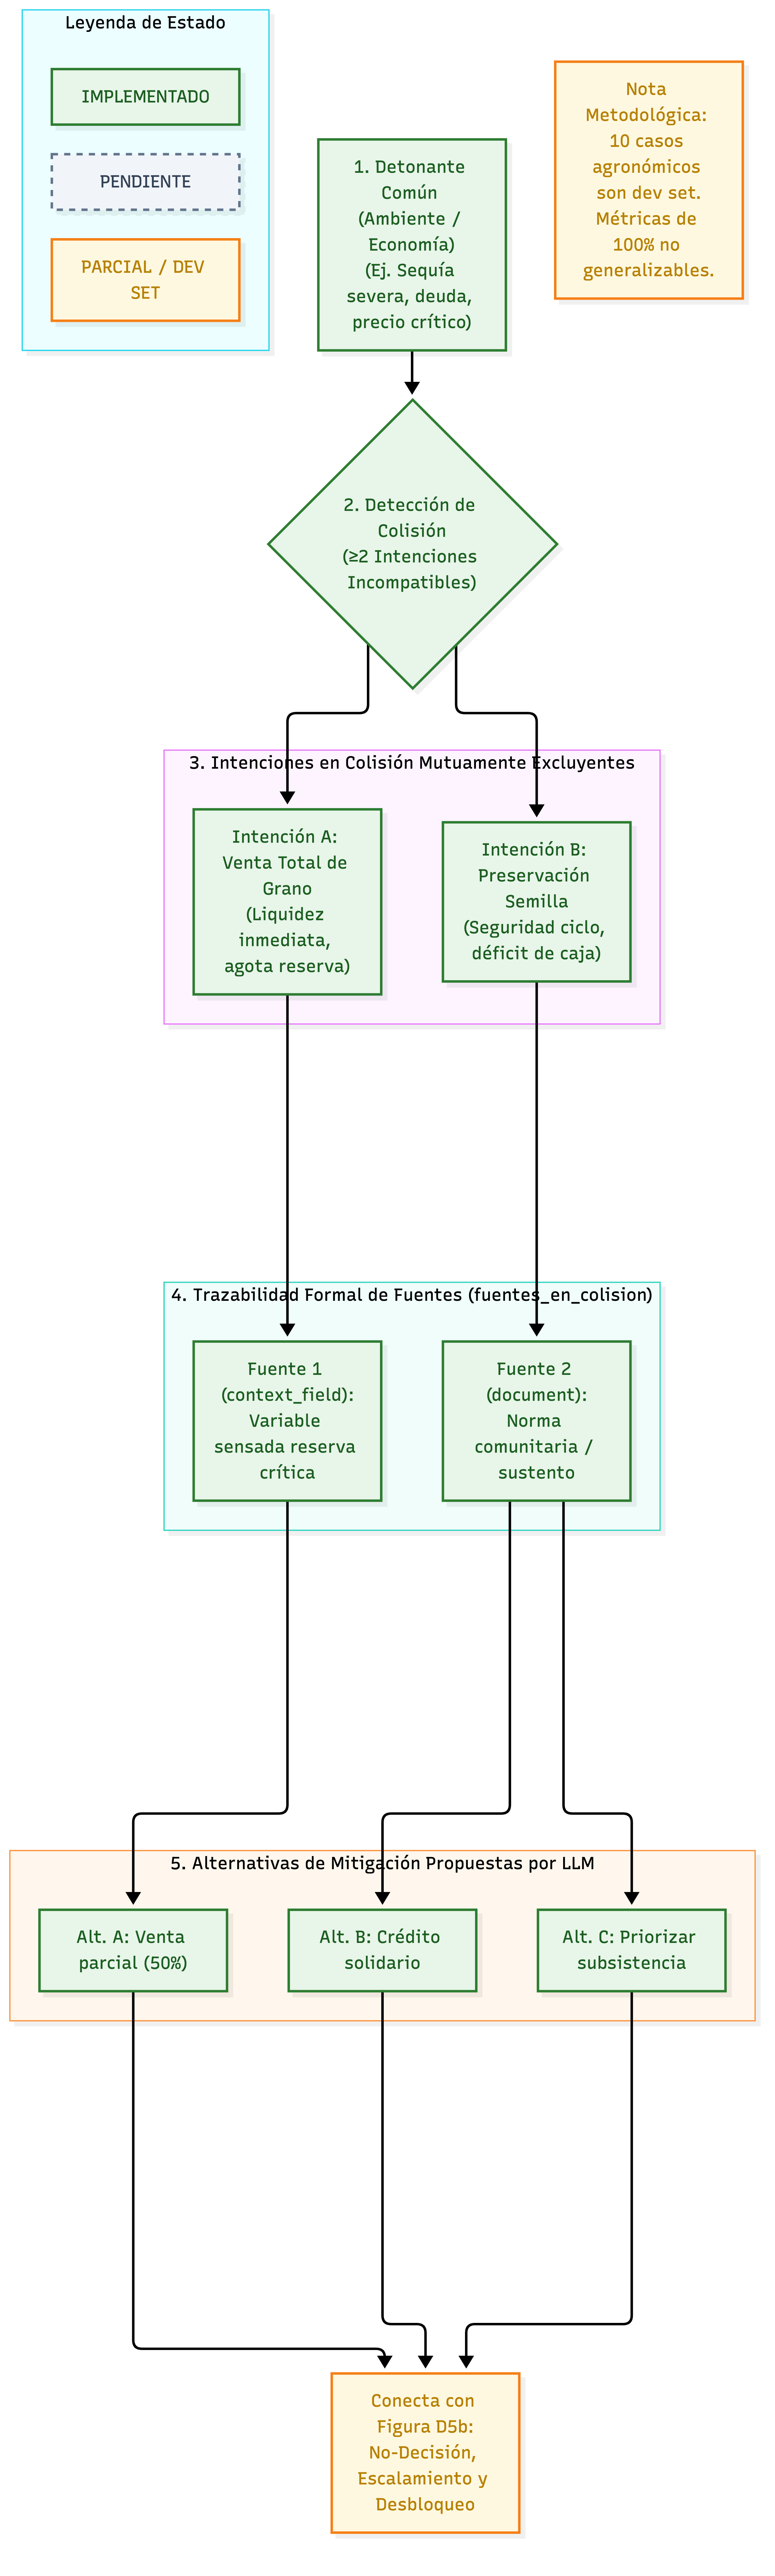
\includegraphics[width=0.88\textwidth,height=0.68\textheight,keepaspectratio]{docs/diagrams/out/d05a_conflict_flow_es.png}
    \caption{Figura D5a. Flujo del Caso Conflictivo (Parte 1: Detección de Colisión y Trazabilidad de Fuentes). Detalla la identificación de colisión entre intenciones agronómicas contradictorias ante un detonante común y el mapeo forense de procedencia (\texttt{context\_field} vs. \texttt{document}). Conecta con el punto B (Figura D5b).}
    \label{fig:d05a_conflict_flow_es}
\end{figure}

% --- Figura D5b: Flujo del Caso Conflictivo (Parte 2: Formulación de Alternativas y Escalamiento Humano) ---
\begin{figure}[htbp]
    \centering
    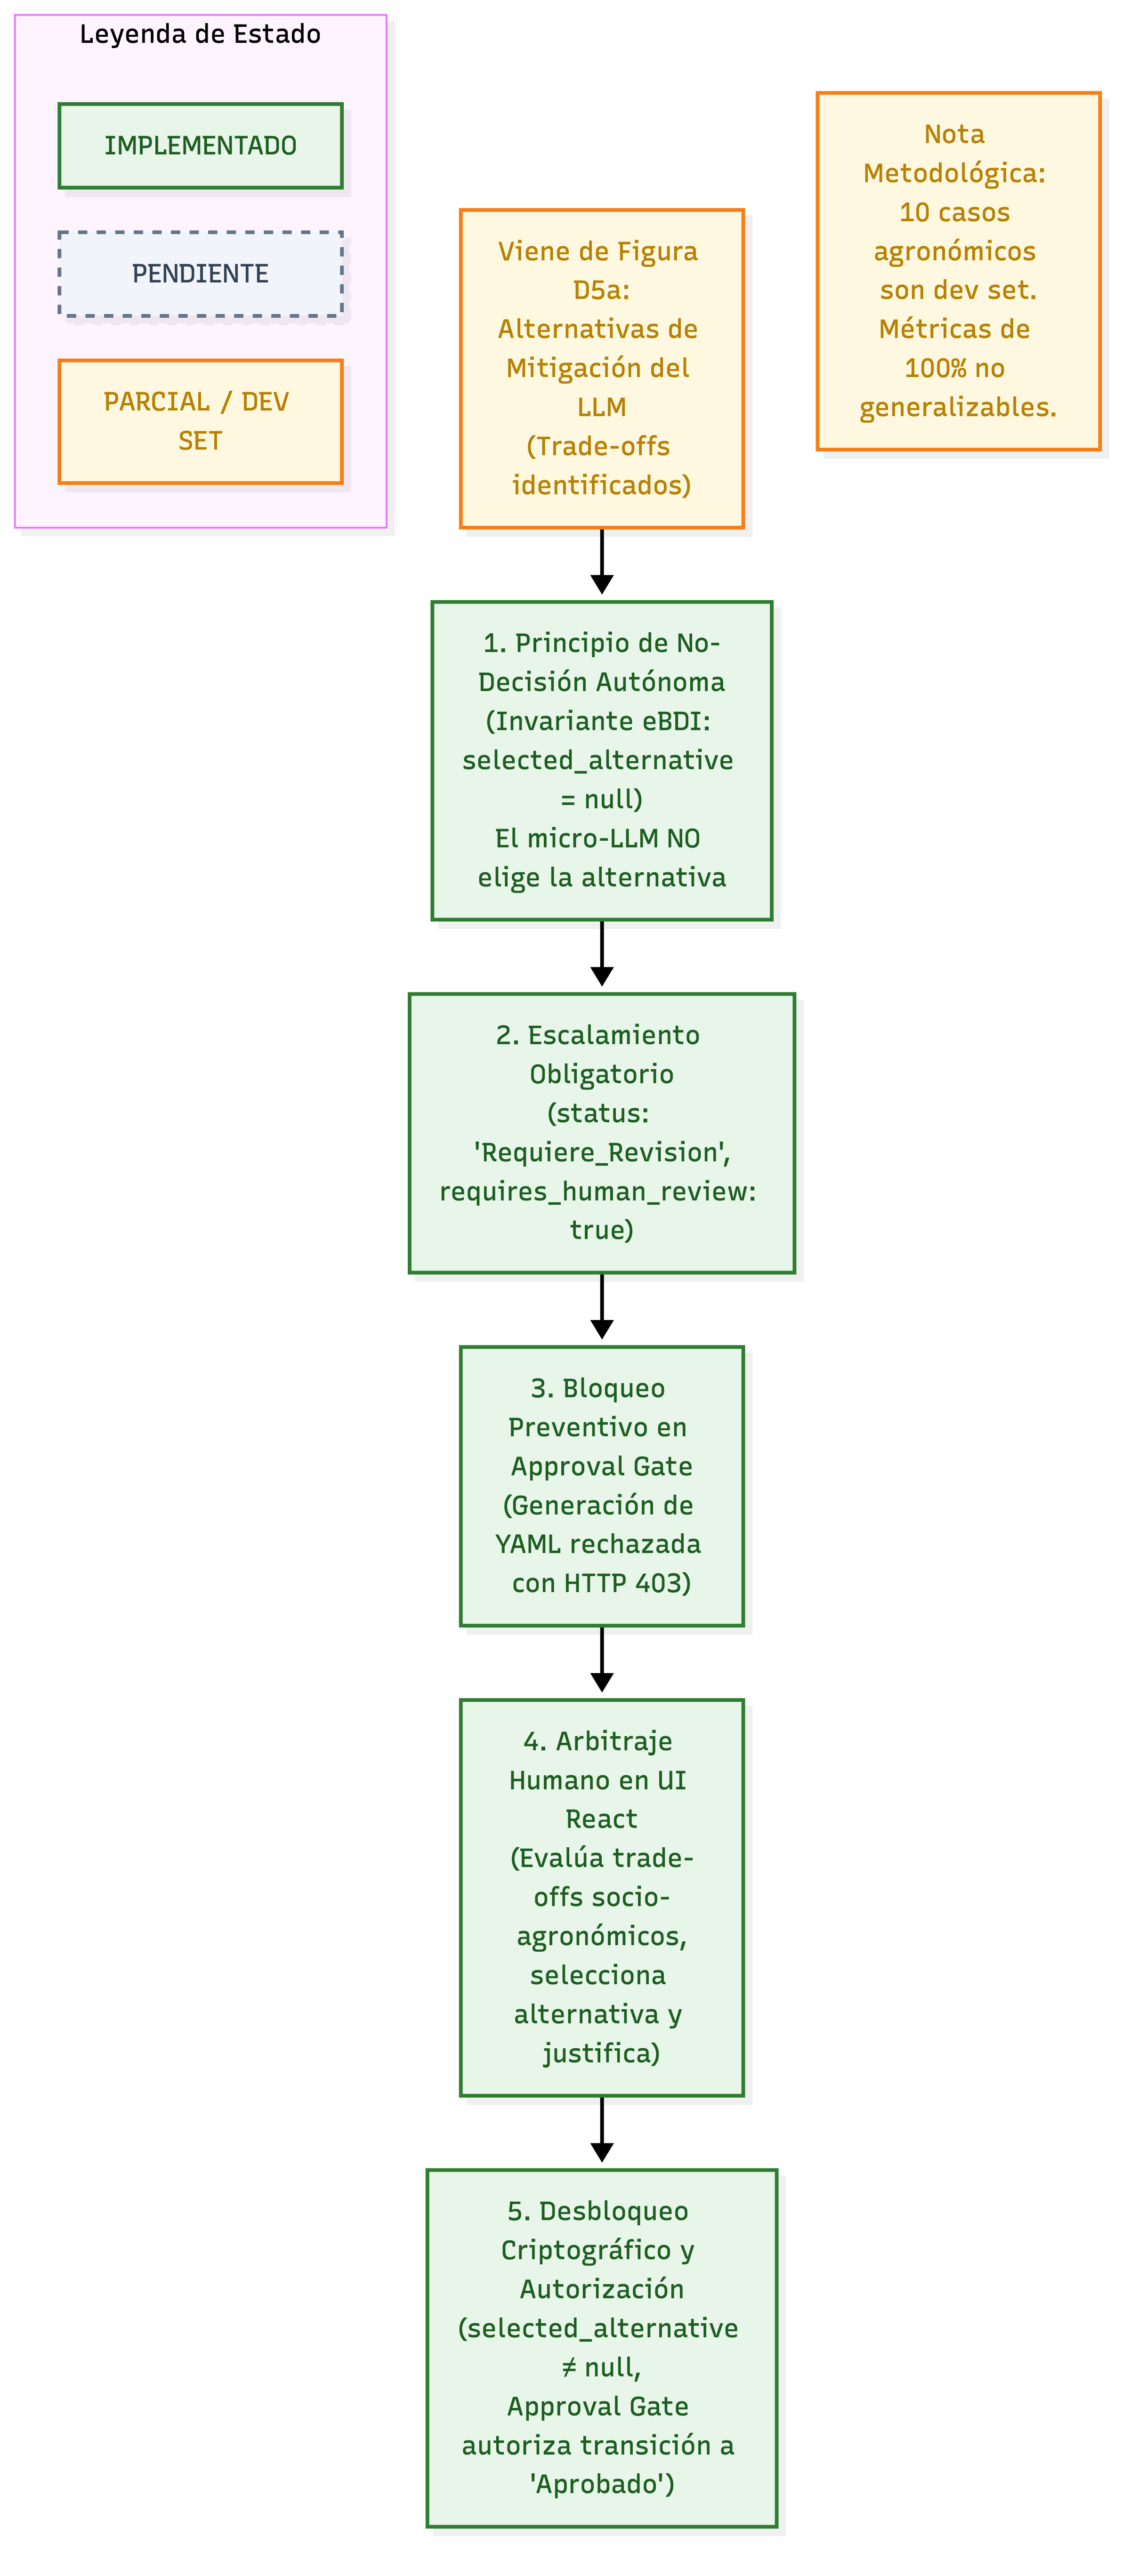
\includegraphics[width=0.88\textwidth,height=0.68\textheight,keepaspectratio]{docs/diagrams/out/d05b_conflict_flow_es.png}
    \caption{Figura D5b. Flujo del Caso Conflictivo (Parte 2: Formulación de Alternativas y Escalamiento Humano). Retoma desde el punto B (Figura D5a), ilustrando la formulación estructurada de alternativas de mitigación (A/B/C), el principio inviolable de no-decisión (\texttt{selected\_alternative = null}) y la obligatoriedad de escalamiento hacia arbitraje humano.}
    \label{fig:d05b_conflict_flow_es}
\end{figure}

% --- Figura D7: Secuencia del Approval Gate (Página Apaisada) ---
\begin{landscape}
\begin{figure}[htbp]
    \centering
    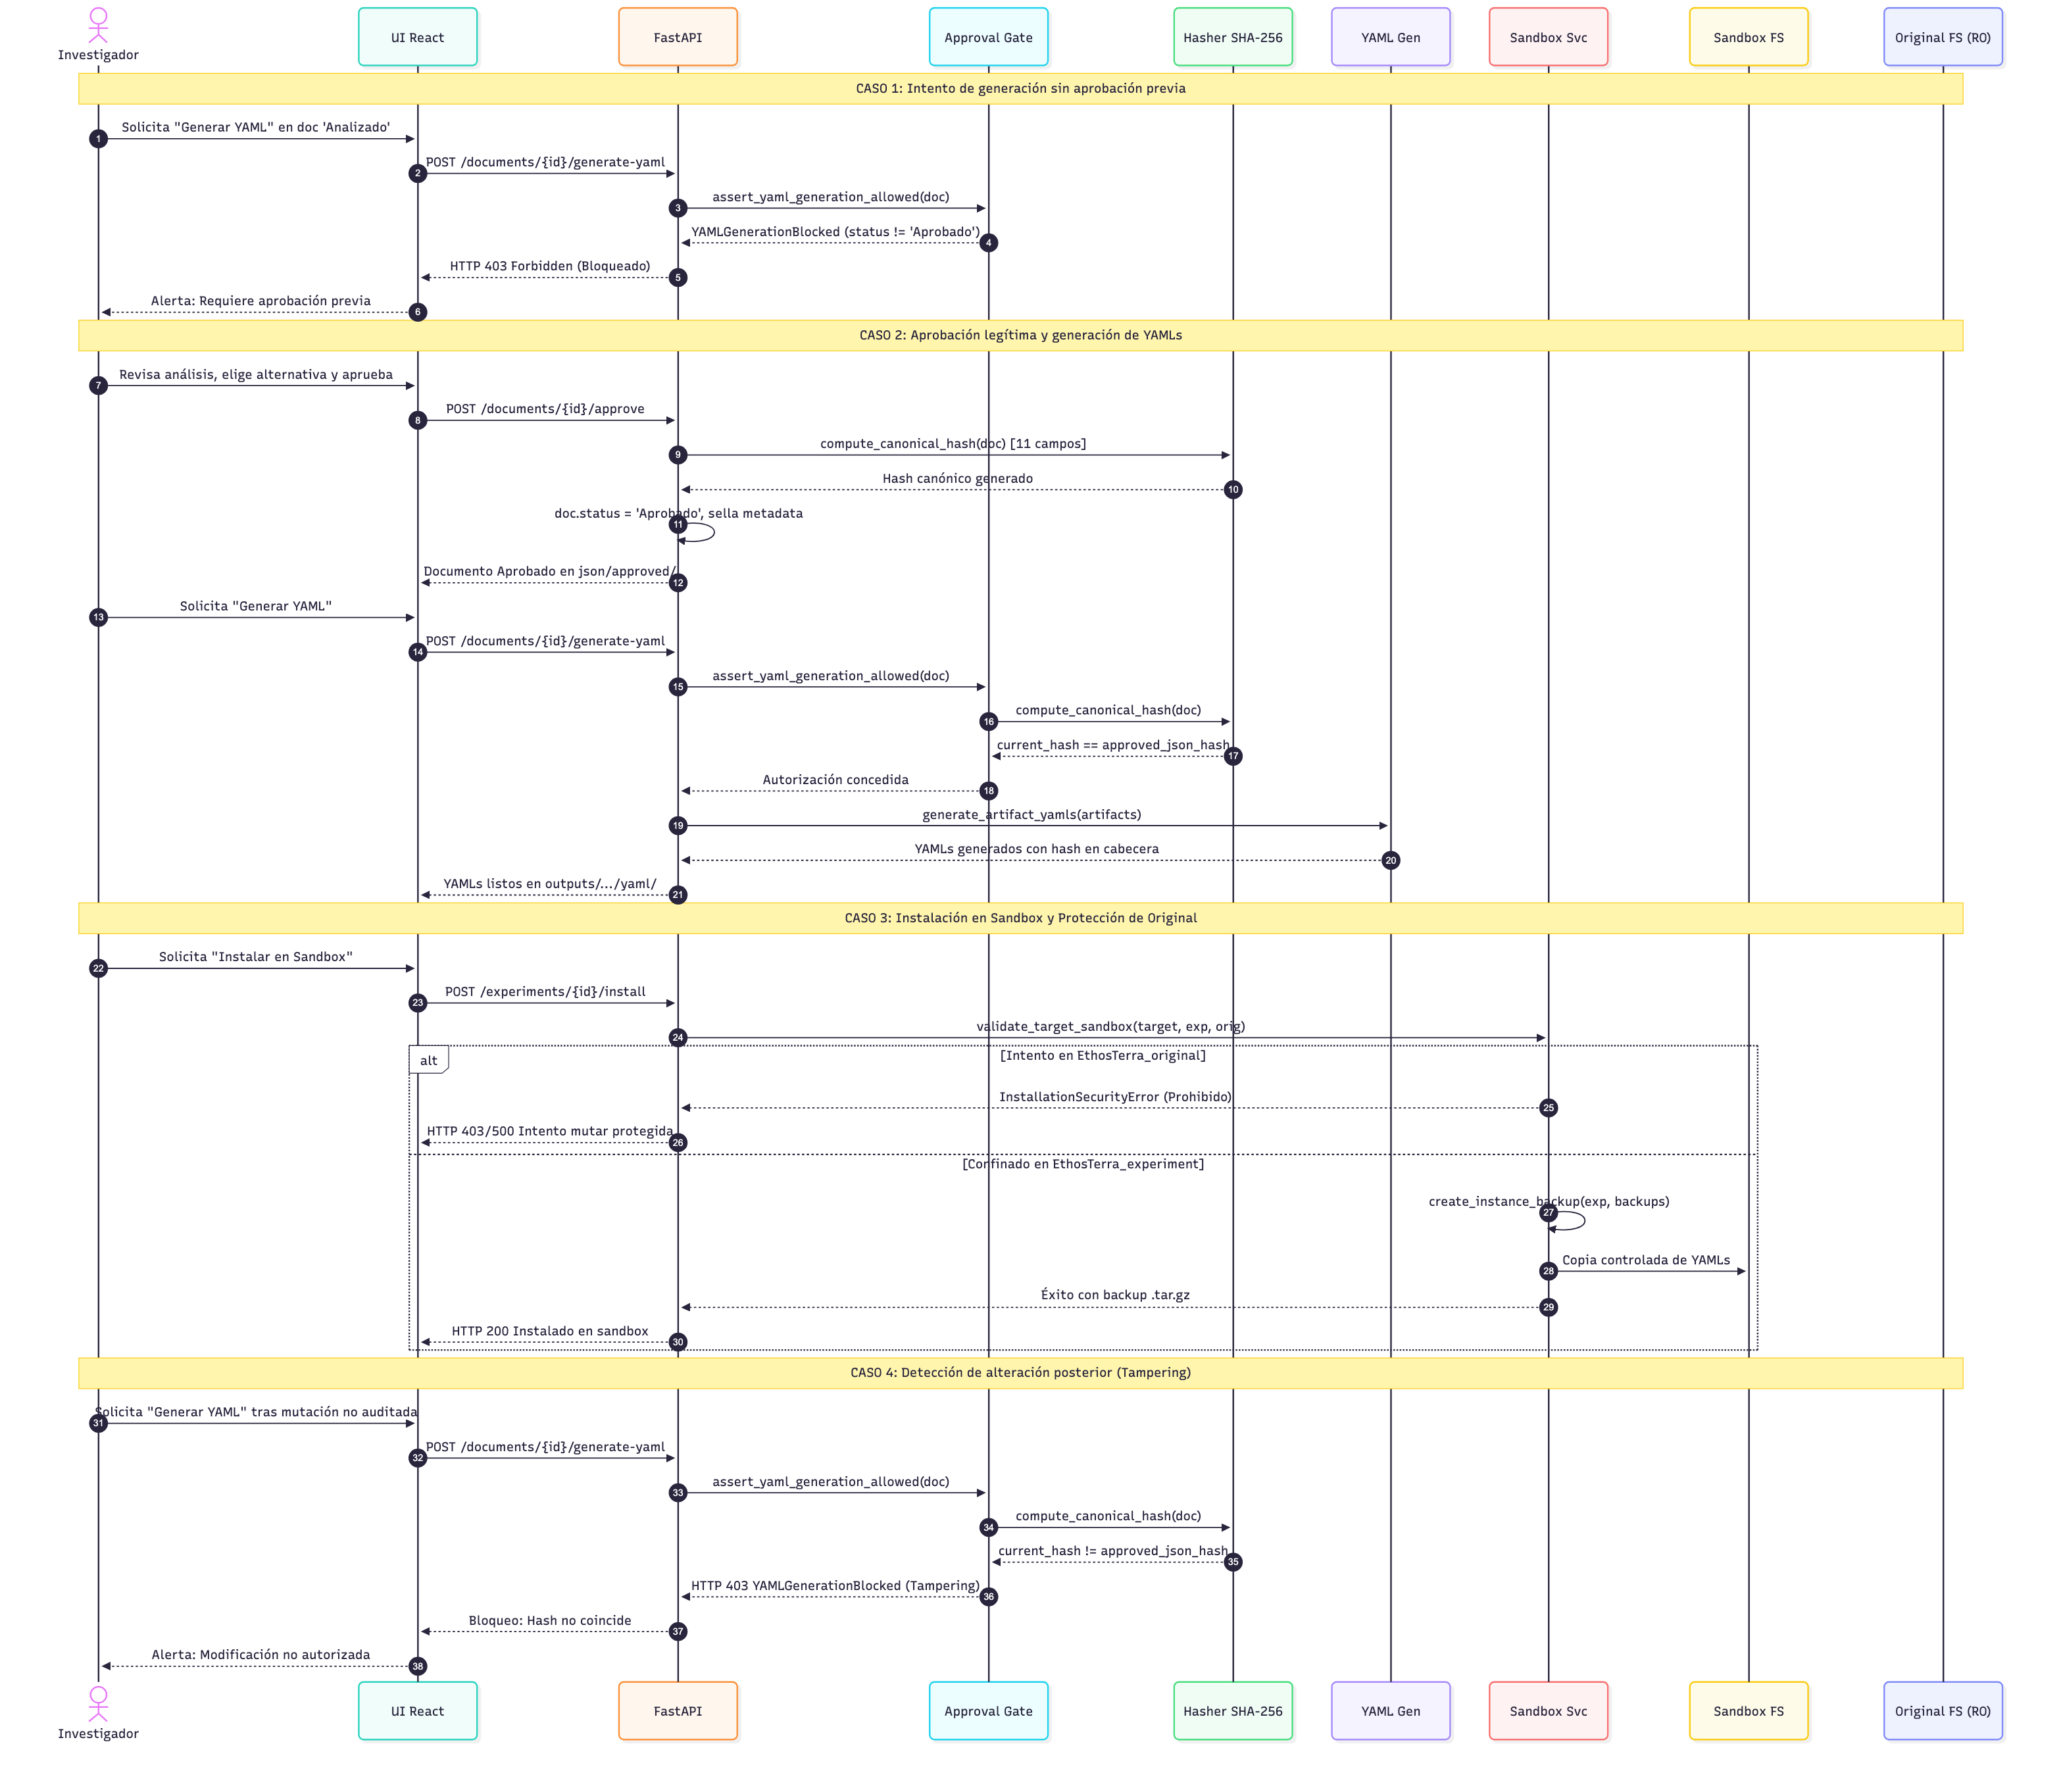
\includegraphics[width=0.95\linewidth,height=0.82\textheight,keepaspectratio]{docs/diagrams/out/d07_approval_gate_seq_es.png}
    \caption{Figura D7. Secuencia del Approval Gate, Compuertas de Seguridad y Sandbox. Detalla la interacción temporal entre el investigador, la UI, la API y los servicios de aplicación en 5 escenarios: bloqueo sin aprobación (403), firma legítima con hash canónico, instalación con respaldo .tar.gz, detección de alteración y rollback atómico.}
    \label{fig:d07_approval_gate_seq_es}
\end{figure}
\end{landscape}

% --- Figura D8: Modelo de Datos y Contratos (Página Apaisada) ---
\begin{landscape}
\begin{figure}[htbp]
    \centering
    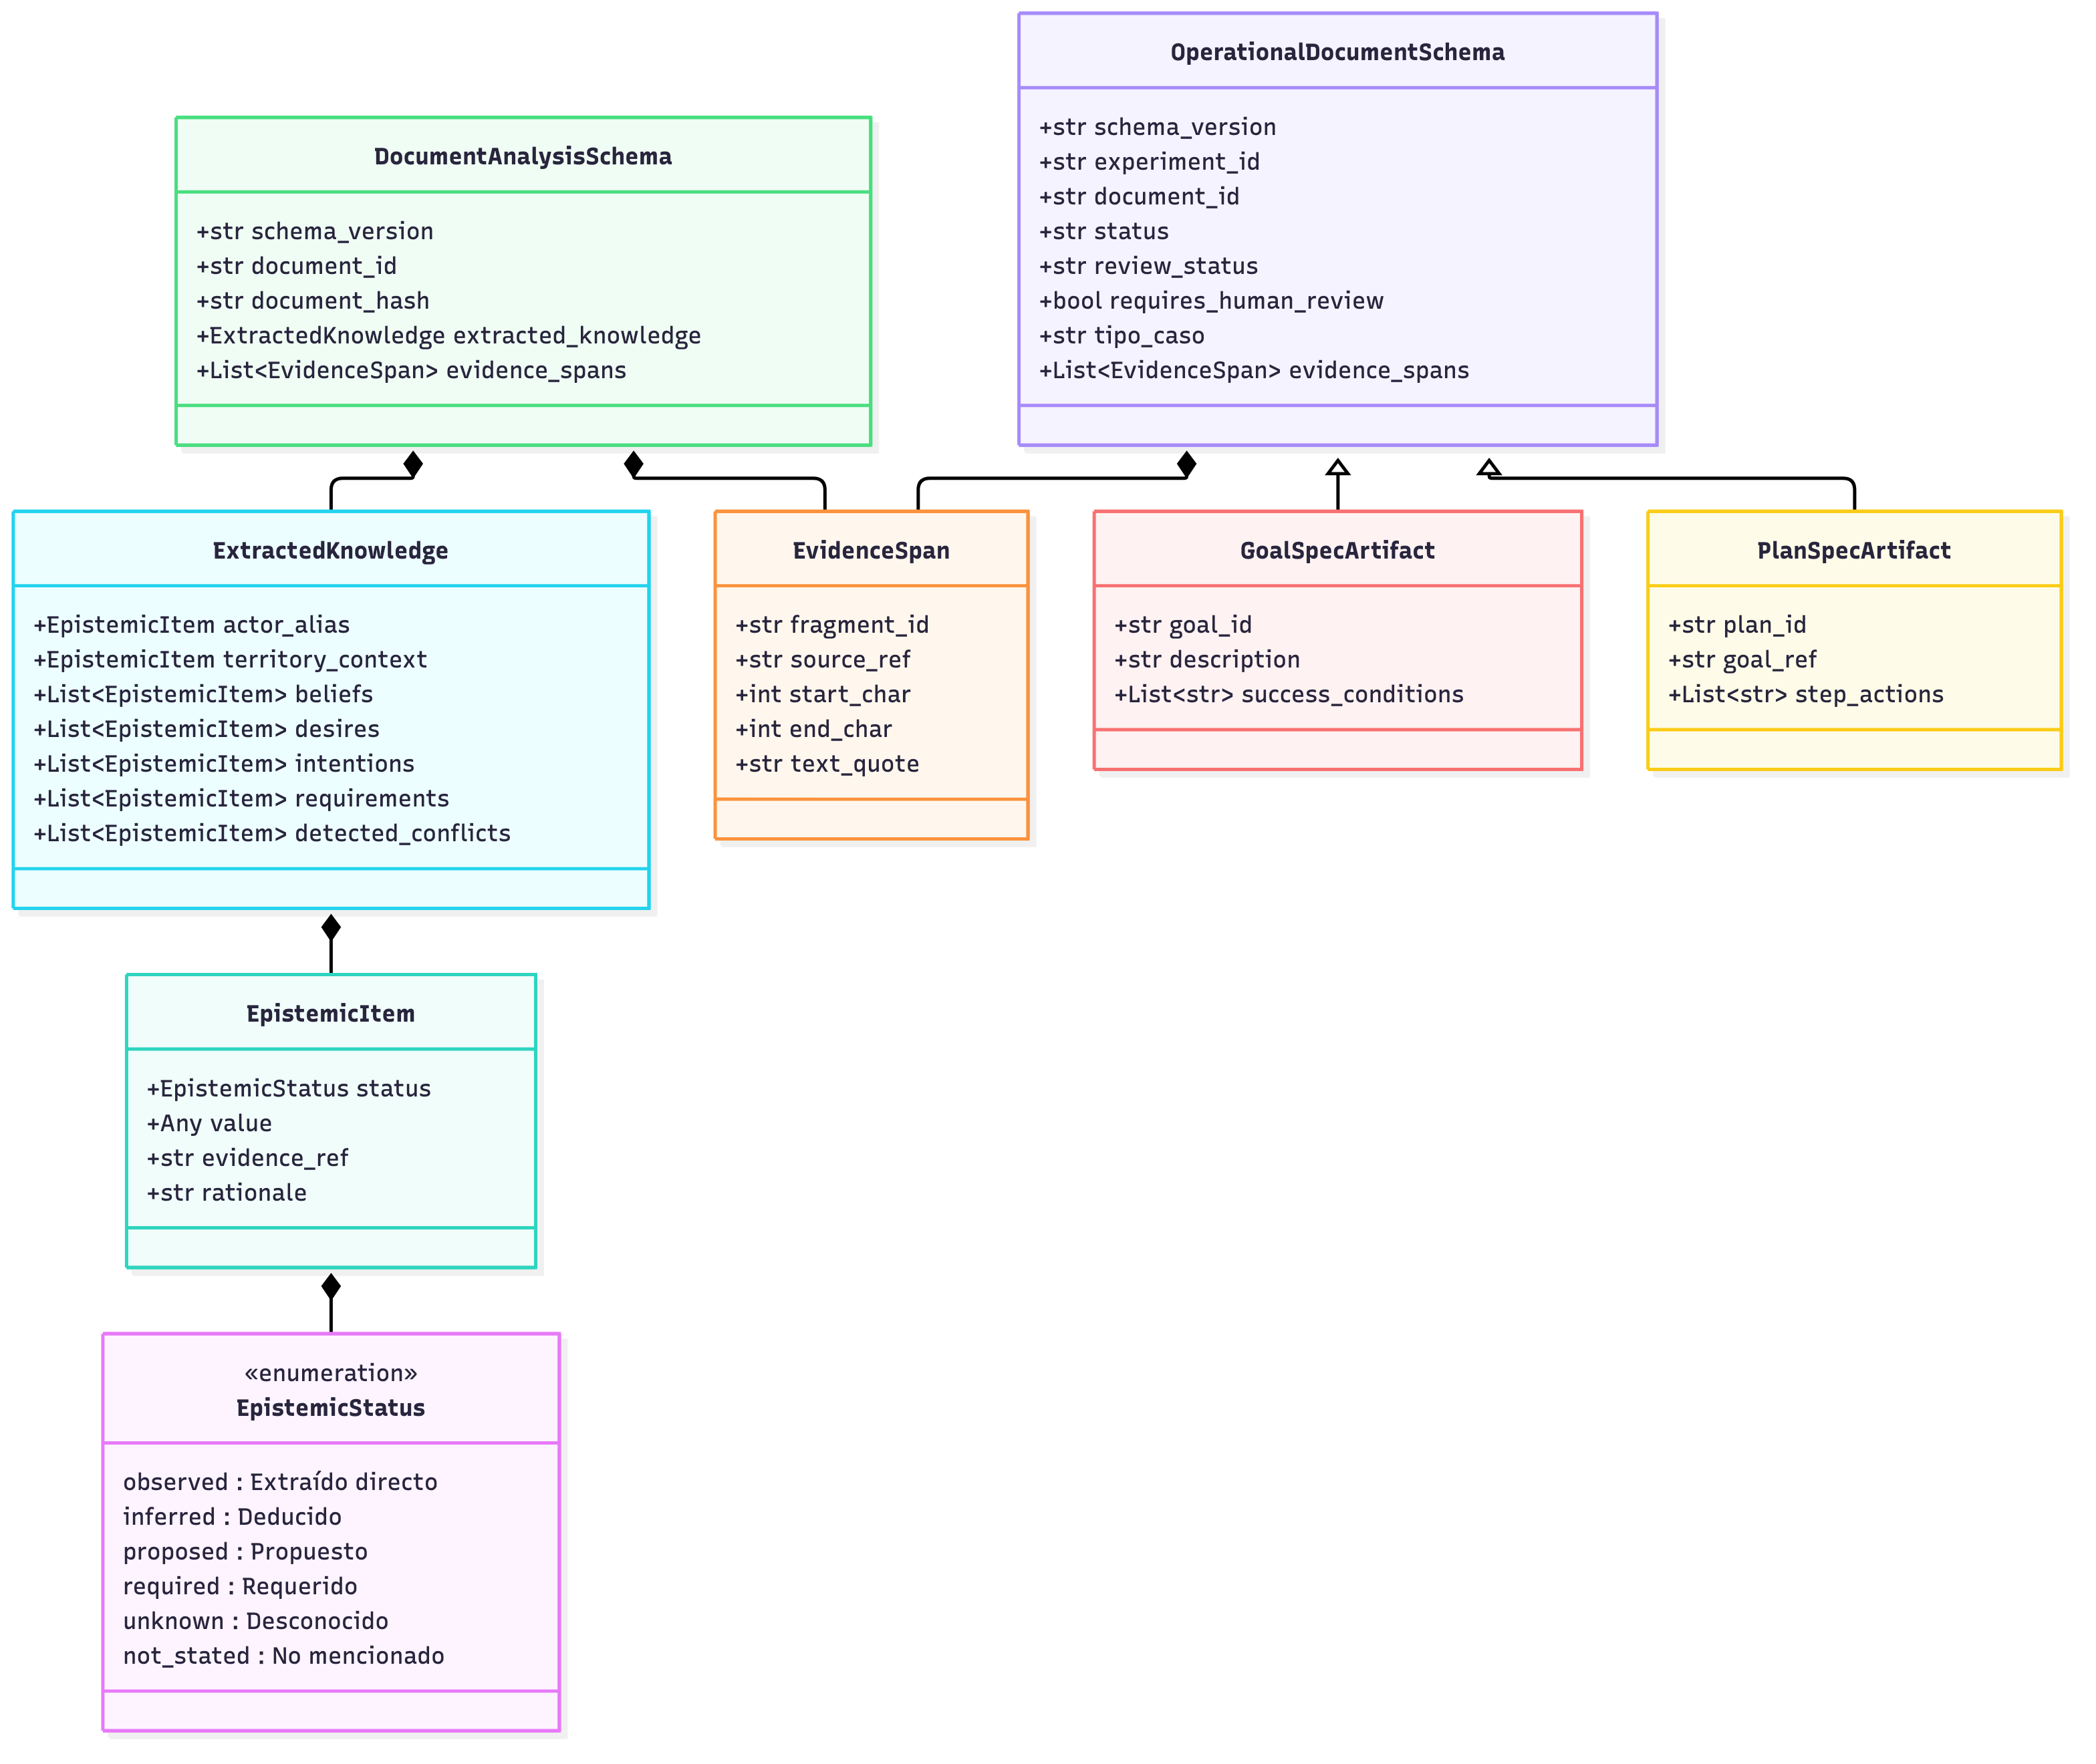
\includegraphics[width=0.95\linewidth,height=0.82\textheight,keepaspectratio]{docs/diagrams/out/d08_data_model_contracts_es.png}
    \caption{Figura D8. Diagrama de Clases del Modelo de Datos y Contratos Pydantic V2. Modela las entidades declarativas \texttt{GoalSpecArtifact}, \texttt{PlanSpecArtifact}, \texttt{OperationalDocumentSchema}, los 6 estados epistemológicos (\texttt{observed}, \texttt{inferred}, \texttt{proposed}, \texttt{required}, \texttt{unknown}, \texttt{not\_stated}) y los fragmentos de evidencia (\texttt{EvidenceSpan}).}
    \label{fig:d08_data_model_contracts_es}
\end{figure}
\end{landscape}

% --- Figura D9a: Despliegue y Entorno (Parte 1: Arquitectura de Procesos y Puertos Locales) ---
\begin{figure}[htbp]
    \centering
    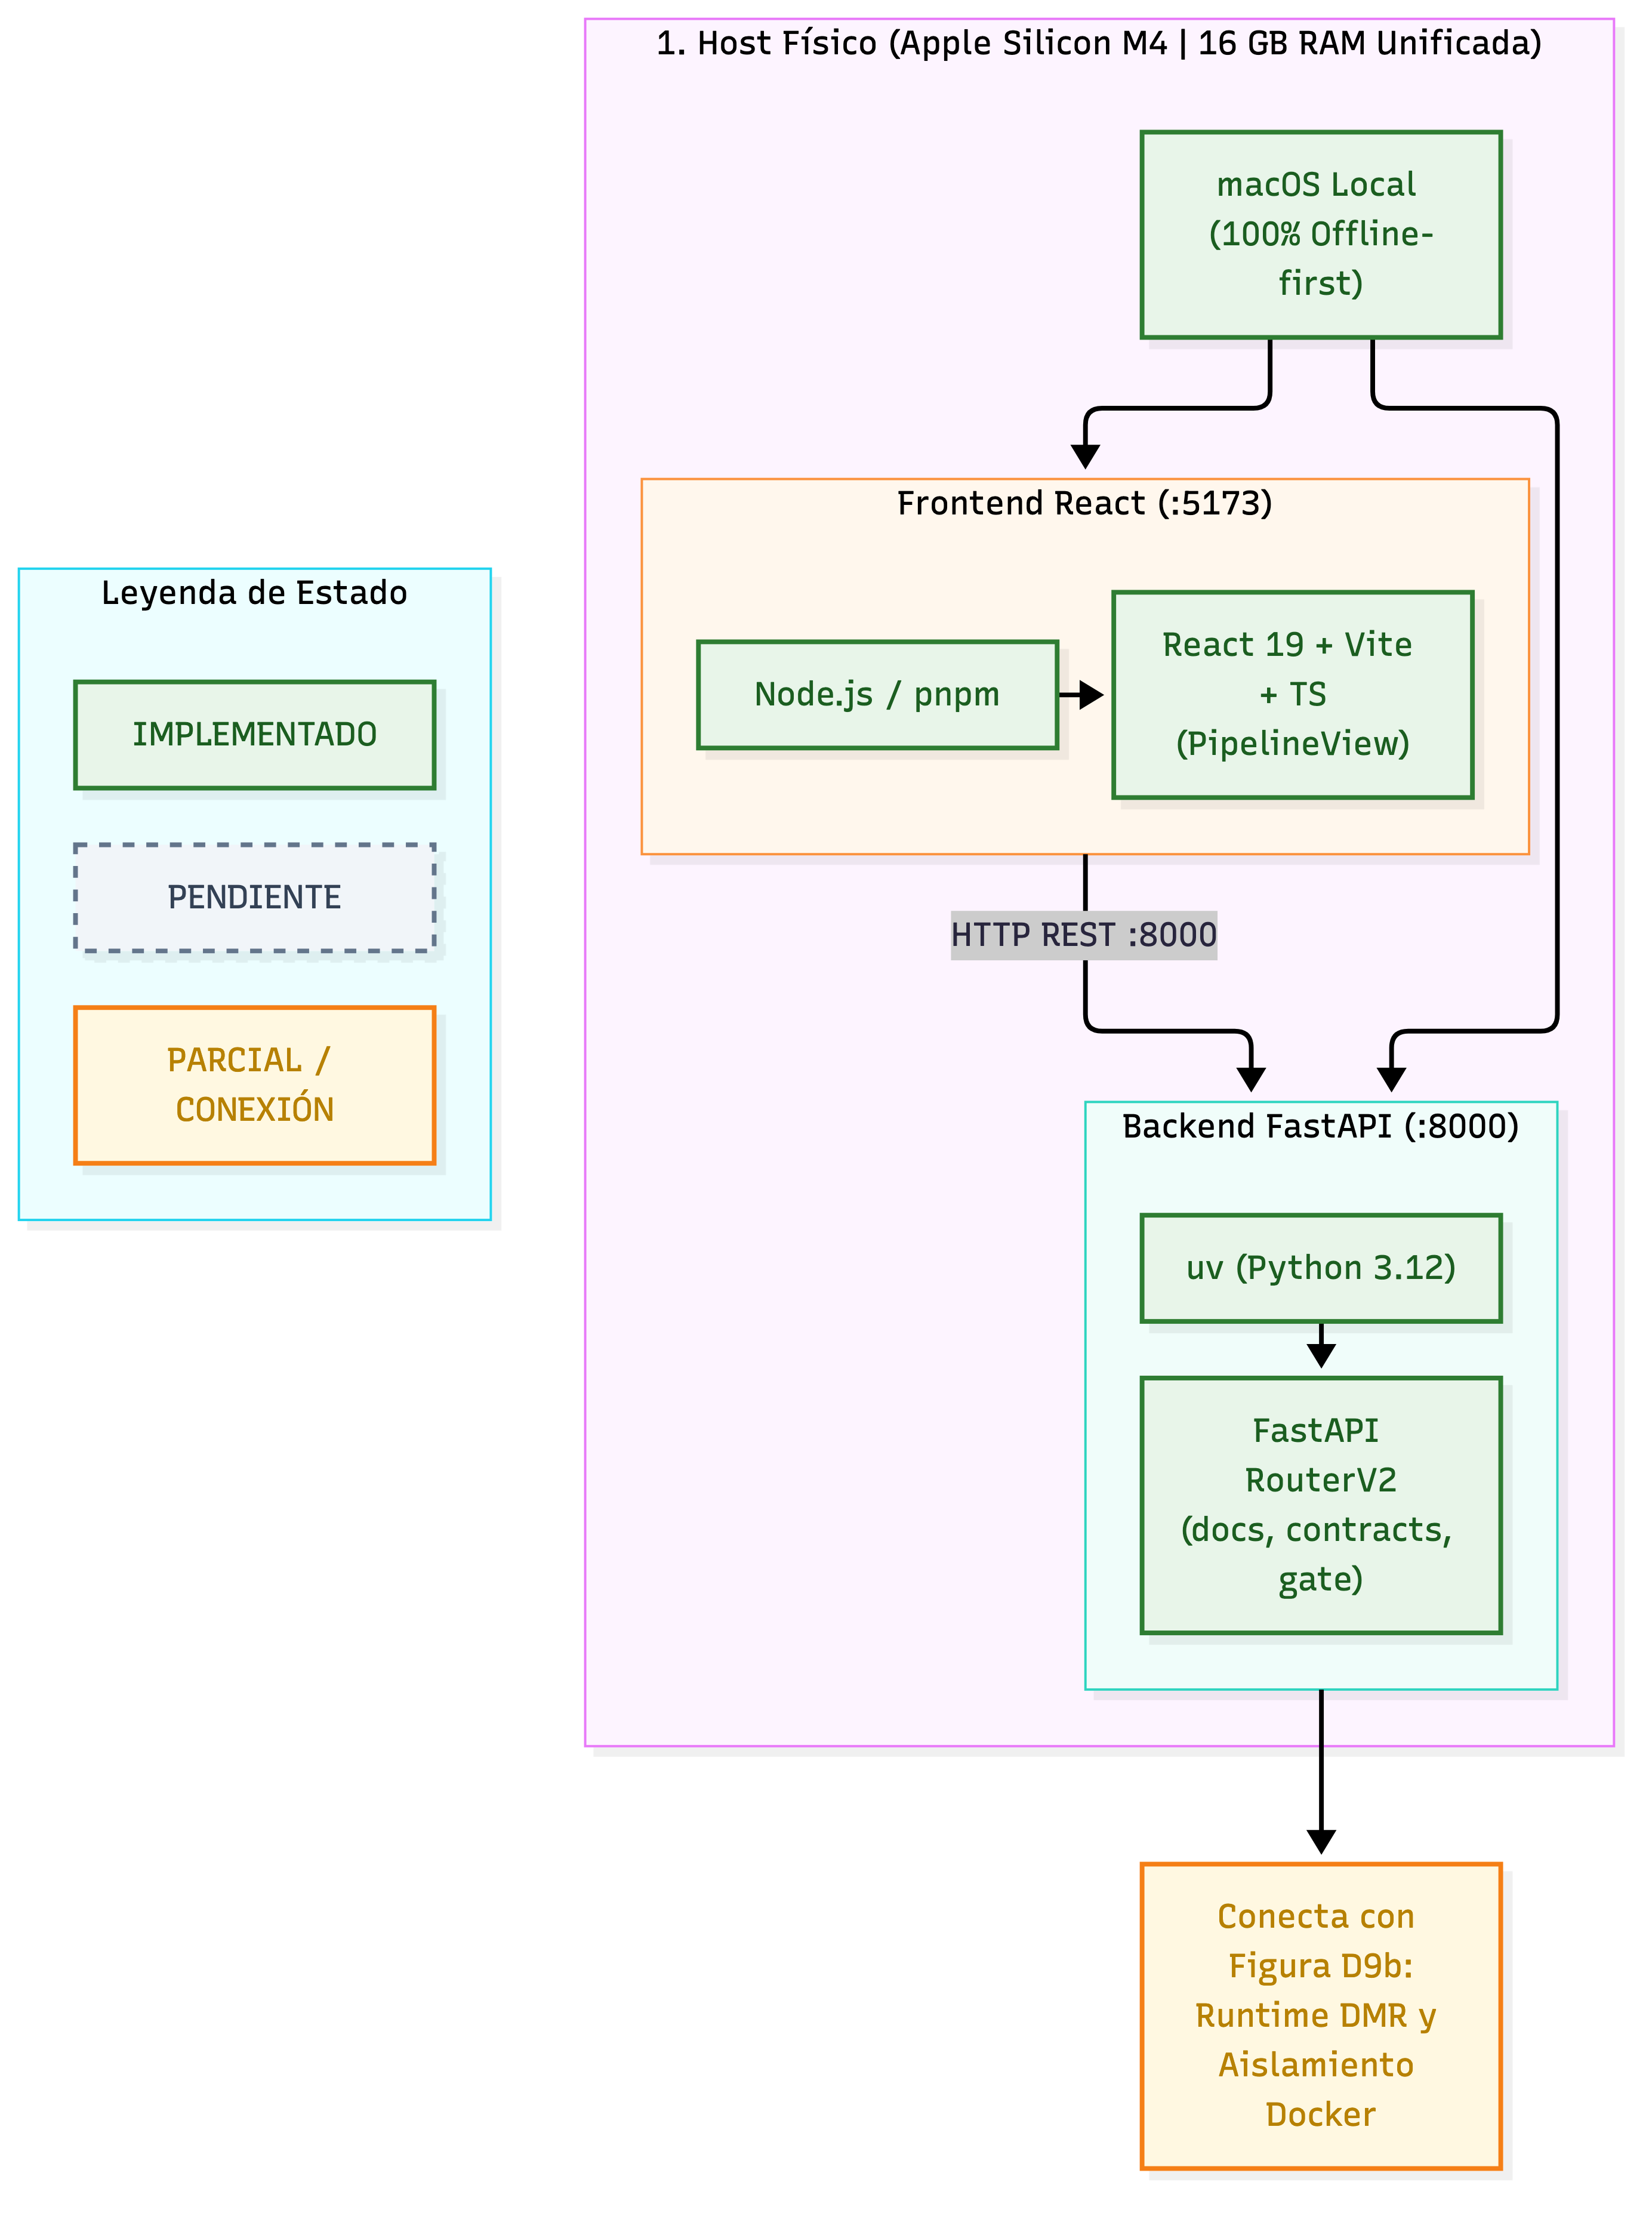
\includegraphics[width=0.88\textwidth,height=0.68\textheight,keepaspectratio]{docs/diagrams/out/d09a_deployment_env_es.png}
    \caption{Figura D9a. Despliegue y Entorno de Ejecución (Parte 1: Arquitectura de Procesos y Puertos Locales). Detalla la topología de servicios en la estación de trabajo física local, especificando los runtimes (Python 3.14 uv, Node.js pnpm) y los puertos de comunicación interna (\texttt{:5173}, \texttt{:8000}, \texttt{:11434}). Conecta con el runtime DMR (Figura D9b).}
    \label{fig:d09a_deployment_env_es}
\end{figure}

% --- Figura D9b: Despliegue y Entorno (Parte 2: Contenerización DMR y Recursos de Hardware) ---
\begin{figure}[htbp]
    \centering
    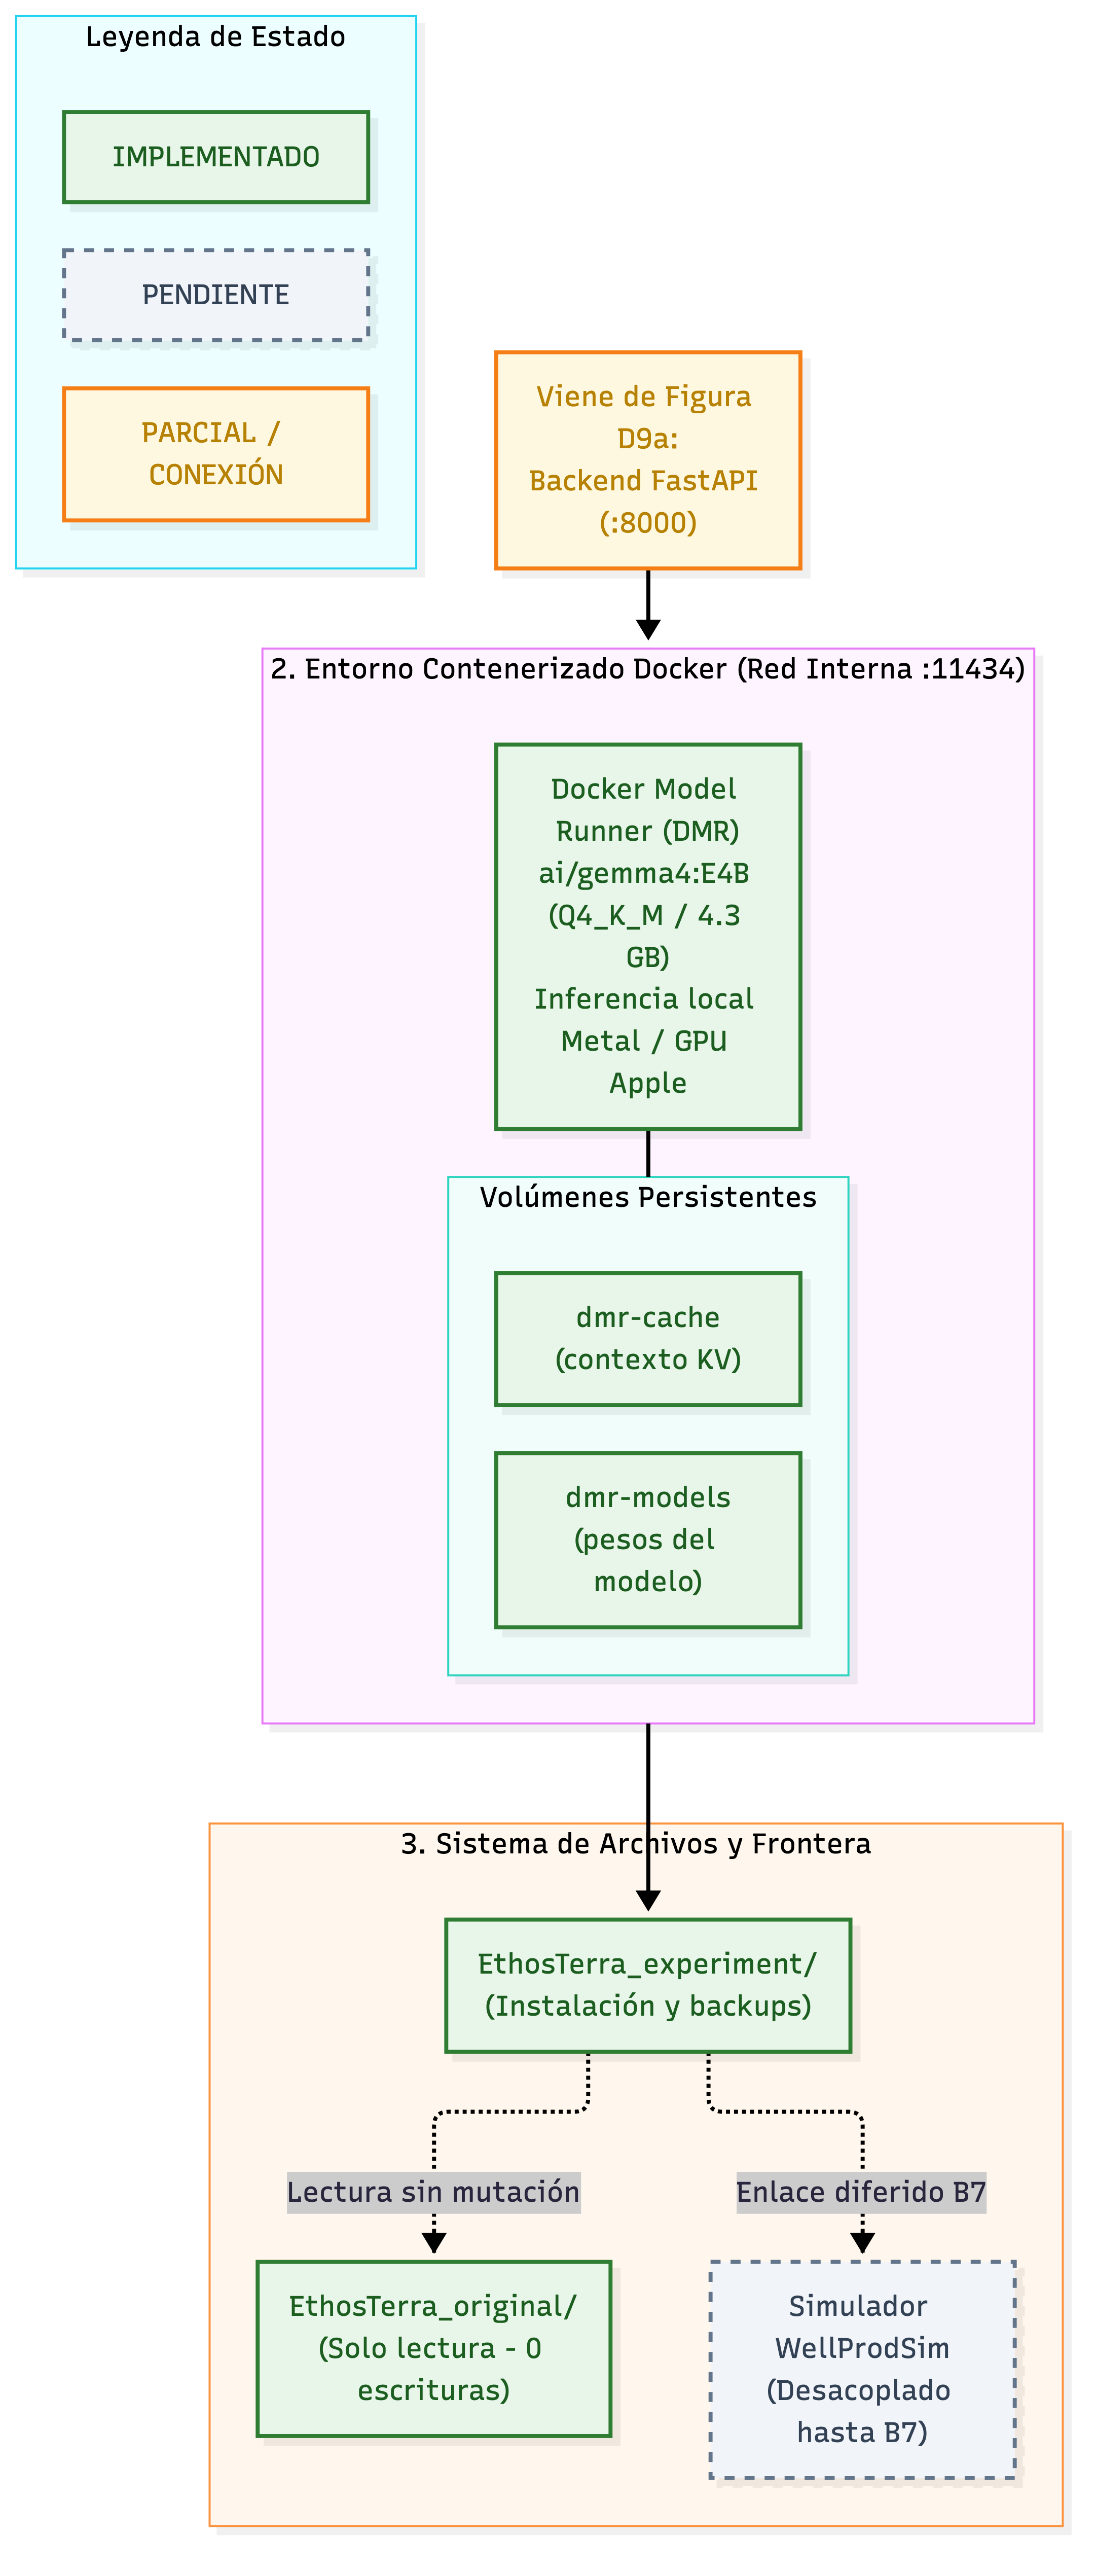
\includegraphics[width=0.88\textwidth,height=0.68\textheight,keepaspectratio]{docs/diagrams/out/d09b_deployment_env_es.png}
    \caption{Figura D9b. Despliegue y Entorno de Ejecución (Parte 2: Contenerización DMR y Recursos de Hardware). Detalla la asignación de memoria unificada en el MacBook Air M4 (16~GB), el contenedor Docker Model Runner, la carga offline de \texttt{ai/gemma4:E4B} y la salvedad sobre el servidor GPU de 24~GB reservado para experimentación a gran escala.}
    \label{fig:d09b_deployment_env_es}
\end{figure}

% --- Figura D10: Trazabilidad de Artefactos y Evidencia ---
\begin{figure}[htbp]
    \centering
    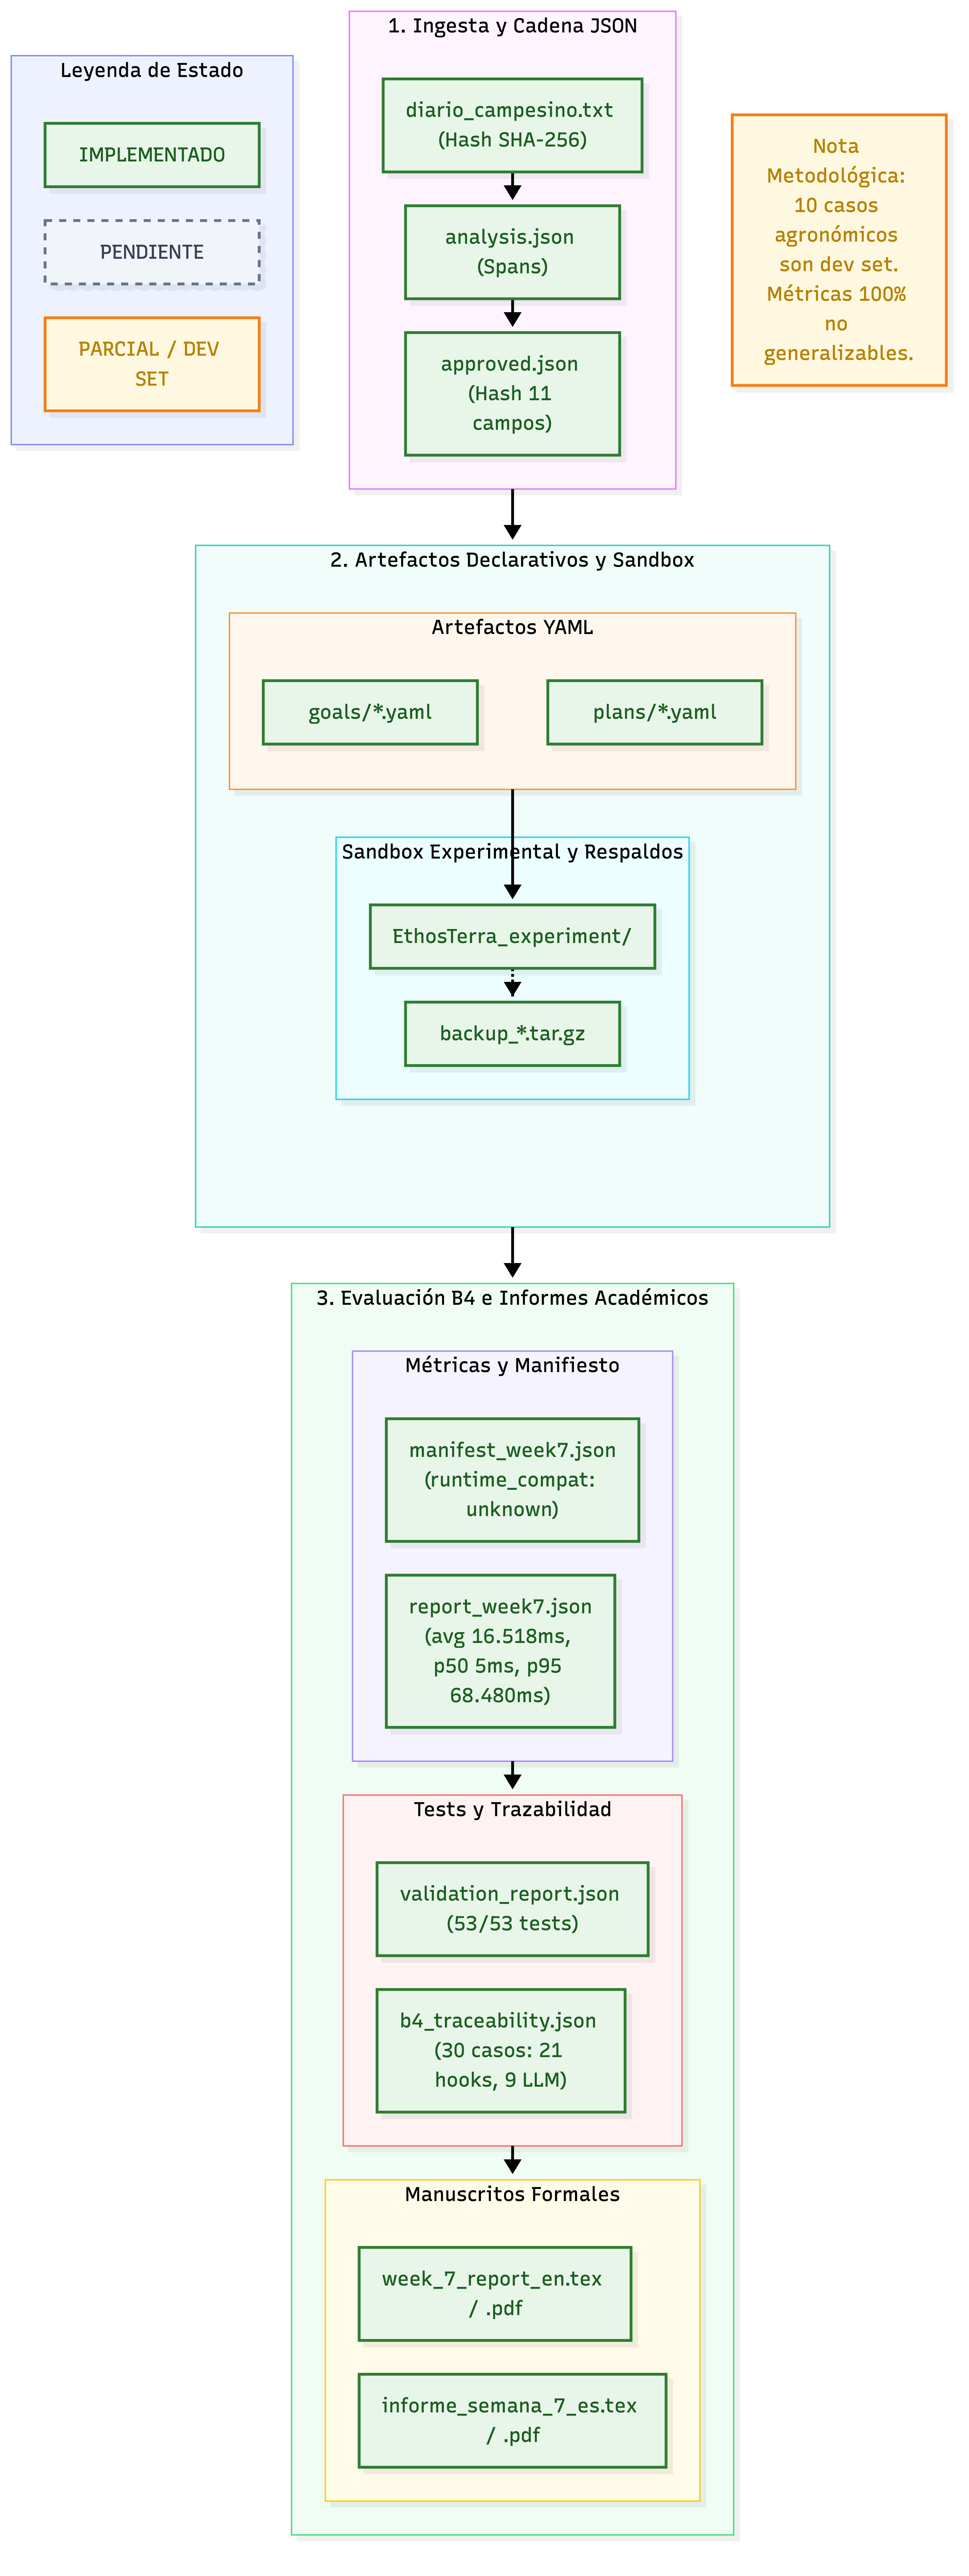
\includegraphics[width=0.88\textwidth,height=0.68\textheight,keepaspectratio]{docs/diagrams/out/d10_artifact_traceability_es.png}
    \caption{Figura D10. Trazabilidad Forense de Artefactos, Evidencias y Reportes. Traza la cadena de custodia completa desde la fuente documental de campo hasta los informes académicos LaTeX, pasando por los esquemas JSON de análisis y aprobación, los archivos YAML generados, backups del sandbox y los manifiestos de evaluación (\texttt{manifest\_week7.json}, \texttt{report\_week7.json}).}
    \label{fig:d10_artifact_traceability_es}
\end{figure}

% --- Figura D12: Vista de Frontera para B5 ---
\begin{figure}[htbp]
    \centering
    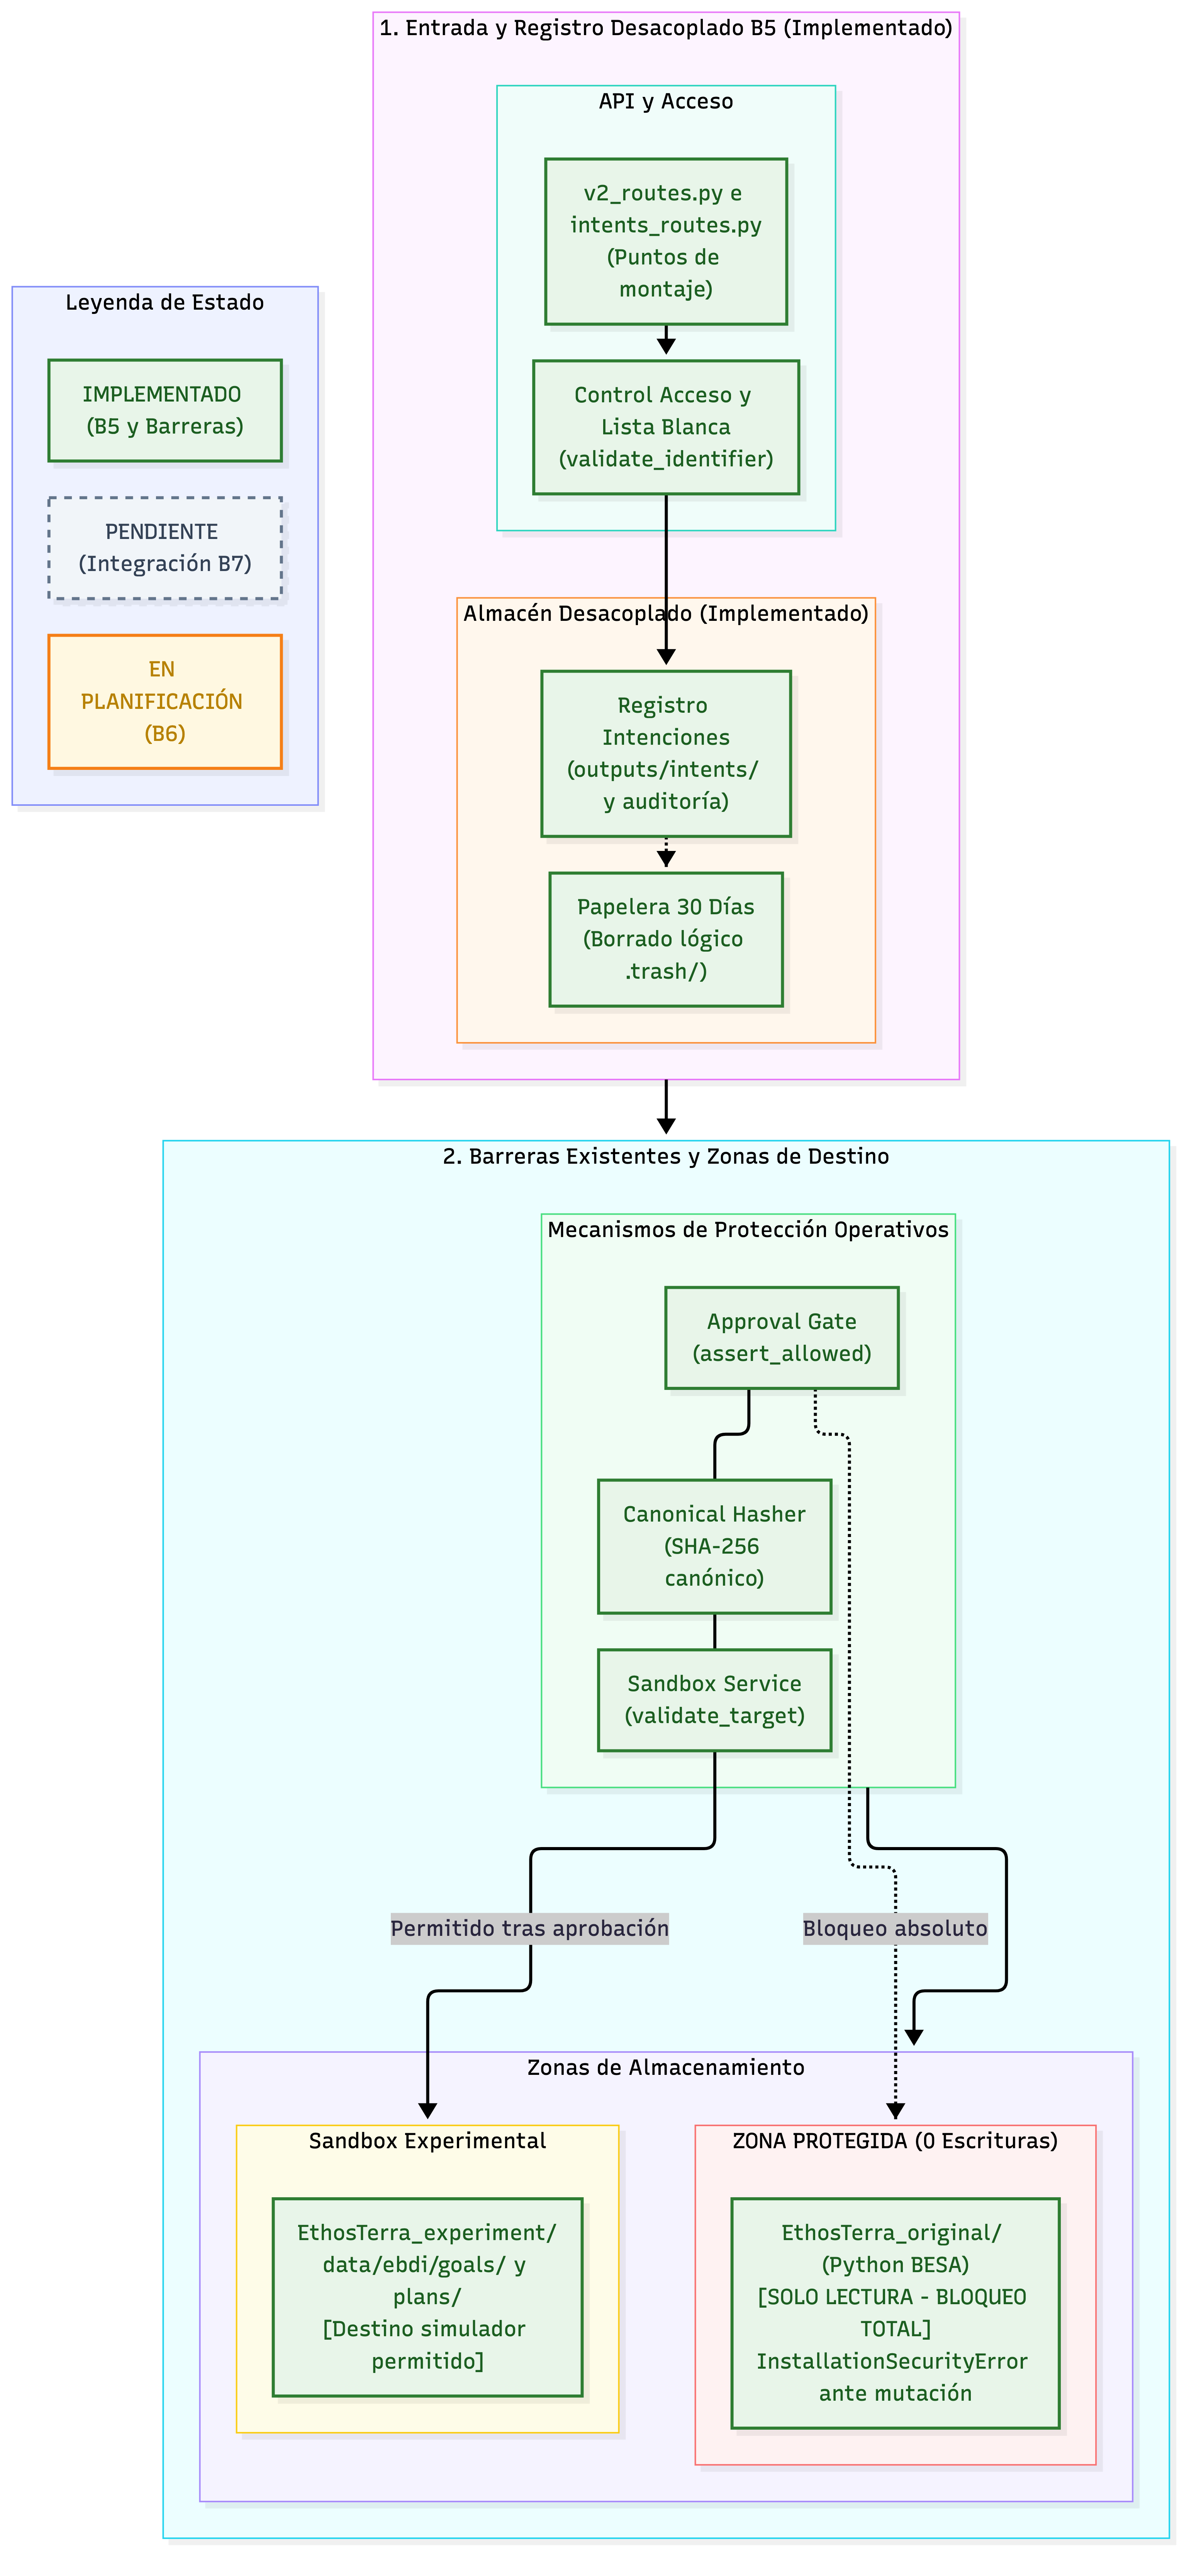
\includegraphics[width=0.88\textwidth,height=0.68\textheight,keepaspectratio]{docs/diagrams/out/d12_b5_boundary_es.png}
    \caption{Figura D12. Frontera Arquitectónica para B5 (CRUD Manual de Intenciones). El registro desacoplado de intenciones en \texttt{outputs/intents/} y la papelera de borrado lógico con retención de 30 días están IMPLEMENTADOS como subsistema autónomo con control de acceso por lista blanca y escrituras atómicas. Se preservan estrictamente las barreras operativas (\texttt{Approval Gate}, \texttt{validate\_target\_sandbox}, y \texttt{EthosTerra\_original/} de solo lectura) para garantizar la invariante de 0 escrituras al núcleo.}
    \label{fig:d12_b5_boundary_es}
\end{figure}


\clearpage

% ==============================================================================
% SECTION 3: FIGURES IN ENGLISH — MAIN BODY
% ==============================================================================

% --- Figure D1: General Layered Architecture ---
\begin{figure}[htbp]
    \centering
    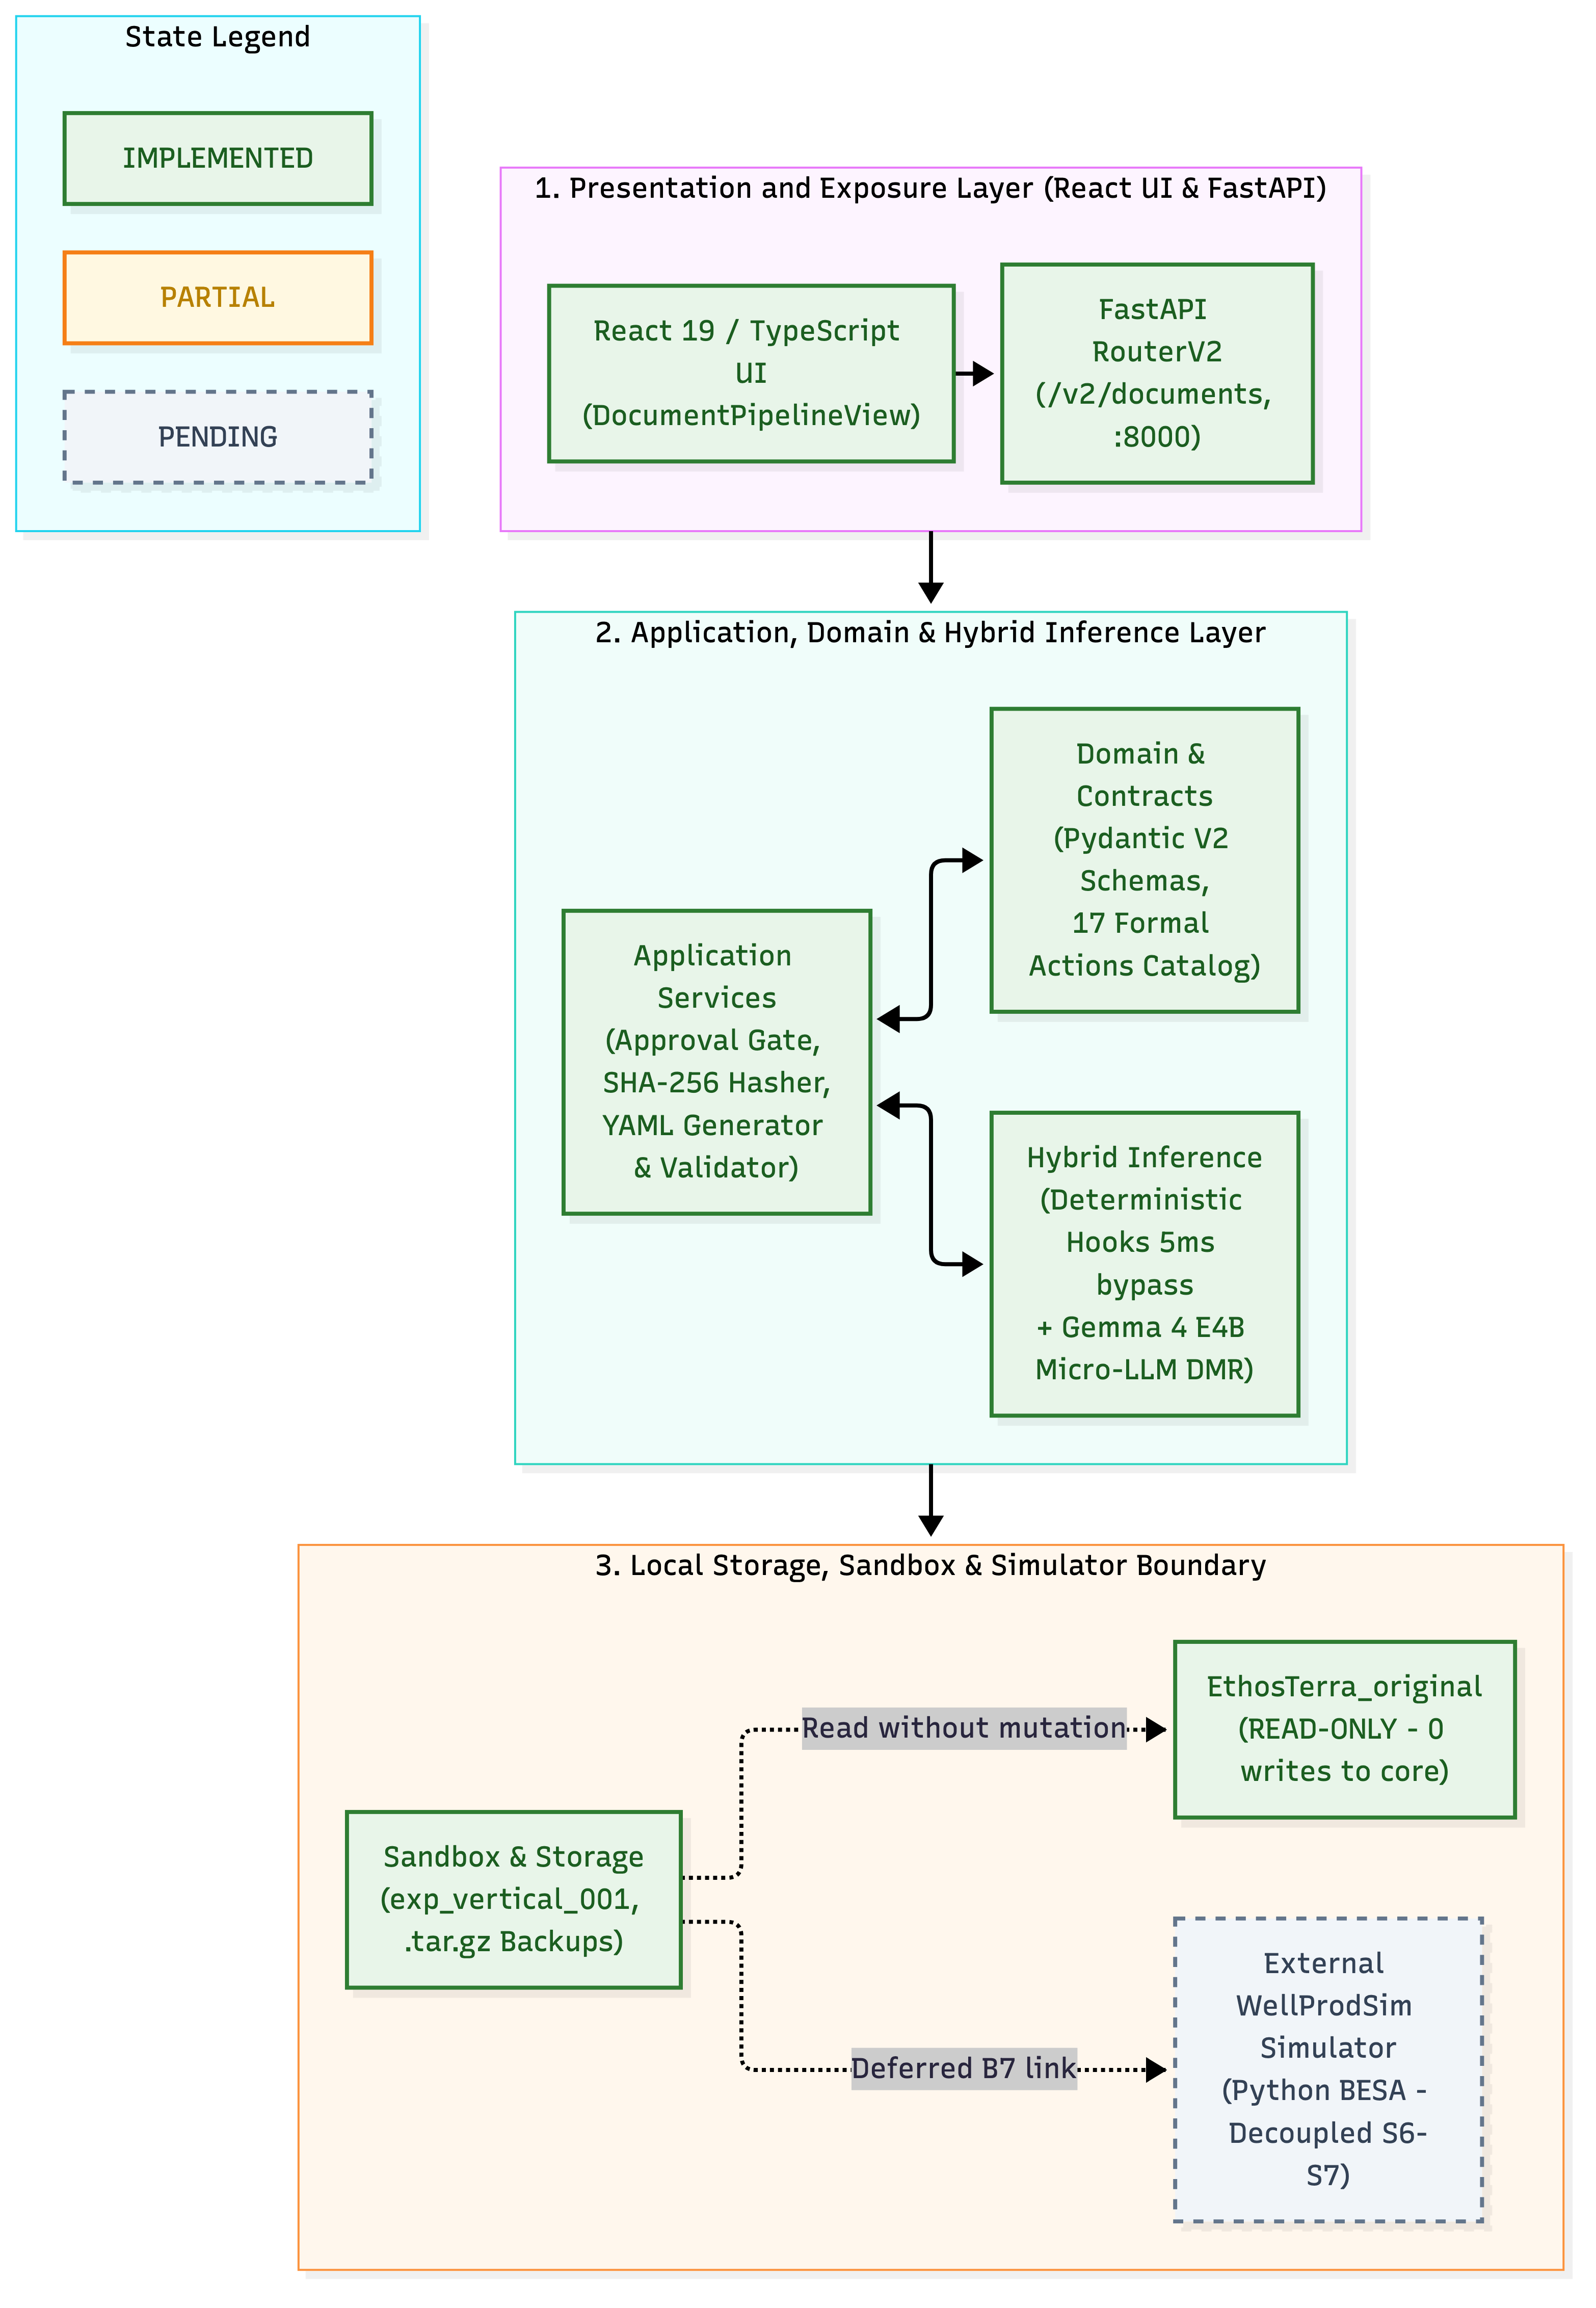
\includegraphics[width=0.88\textwidth,height=0.68\textheight,keepaspectratio]{docs/diagrams/out/d01_arch_layers_en.png}
    \caption{Figure D1. General Layered Architecture of the Hybrid eBDI System. Details the interplay between the React UI, FastAPI exposure layer, application services, domain models, local DMR runtime (offline-first), experimental sandbox, and the decoupled boundary to the external simulator.}
    \label{fig:d01_arch_layers_en}
\end{figure}

% --- Figure D4a: Hybrid Classifier Flow (Part 1: Ingestion, Normalization and Deterministic Bypass) ---
\begin{figure}[htbp]
    \centering
    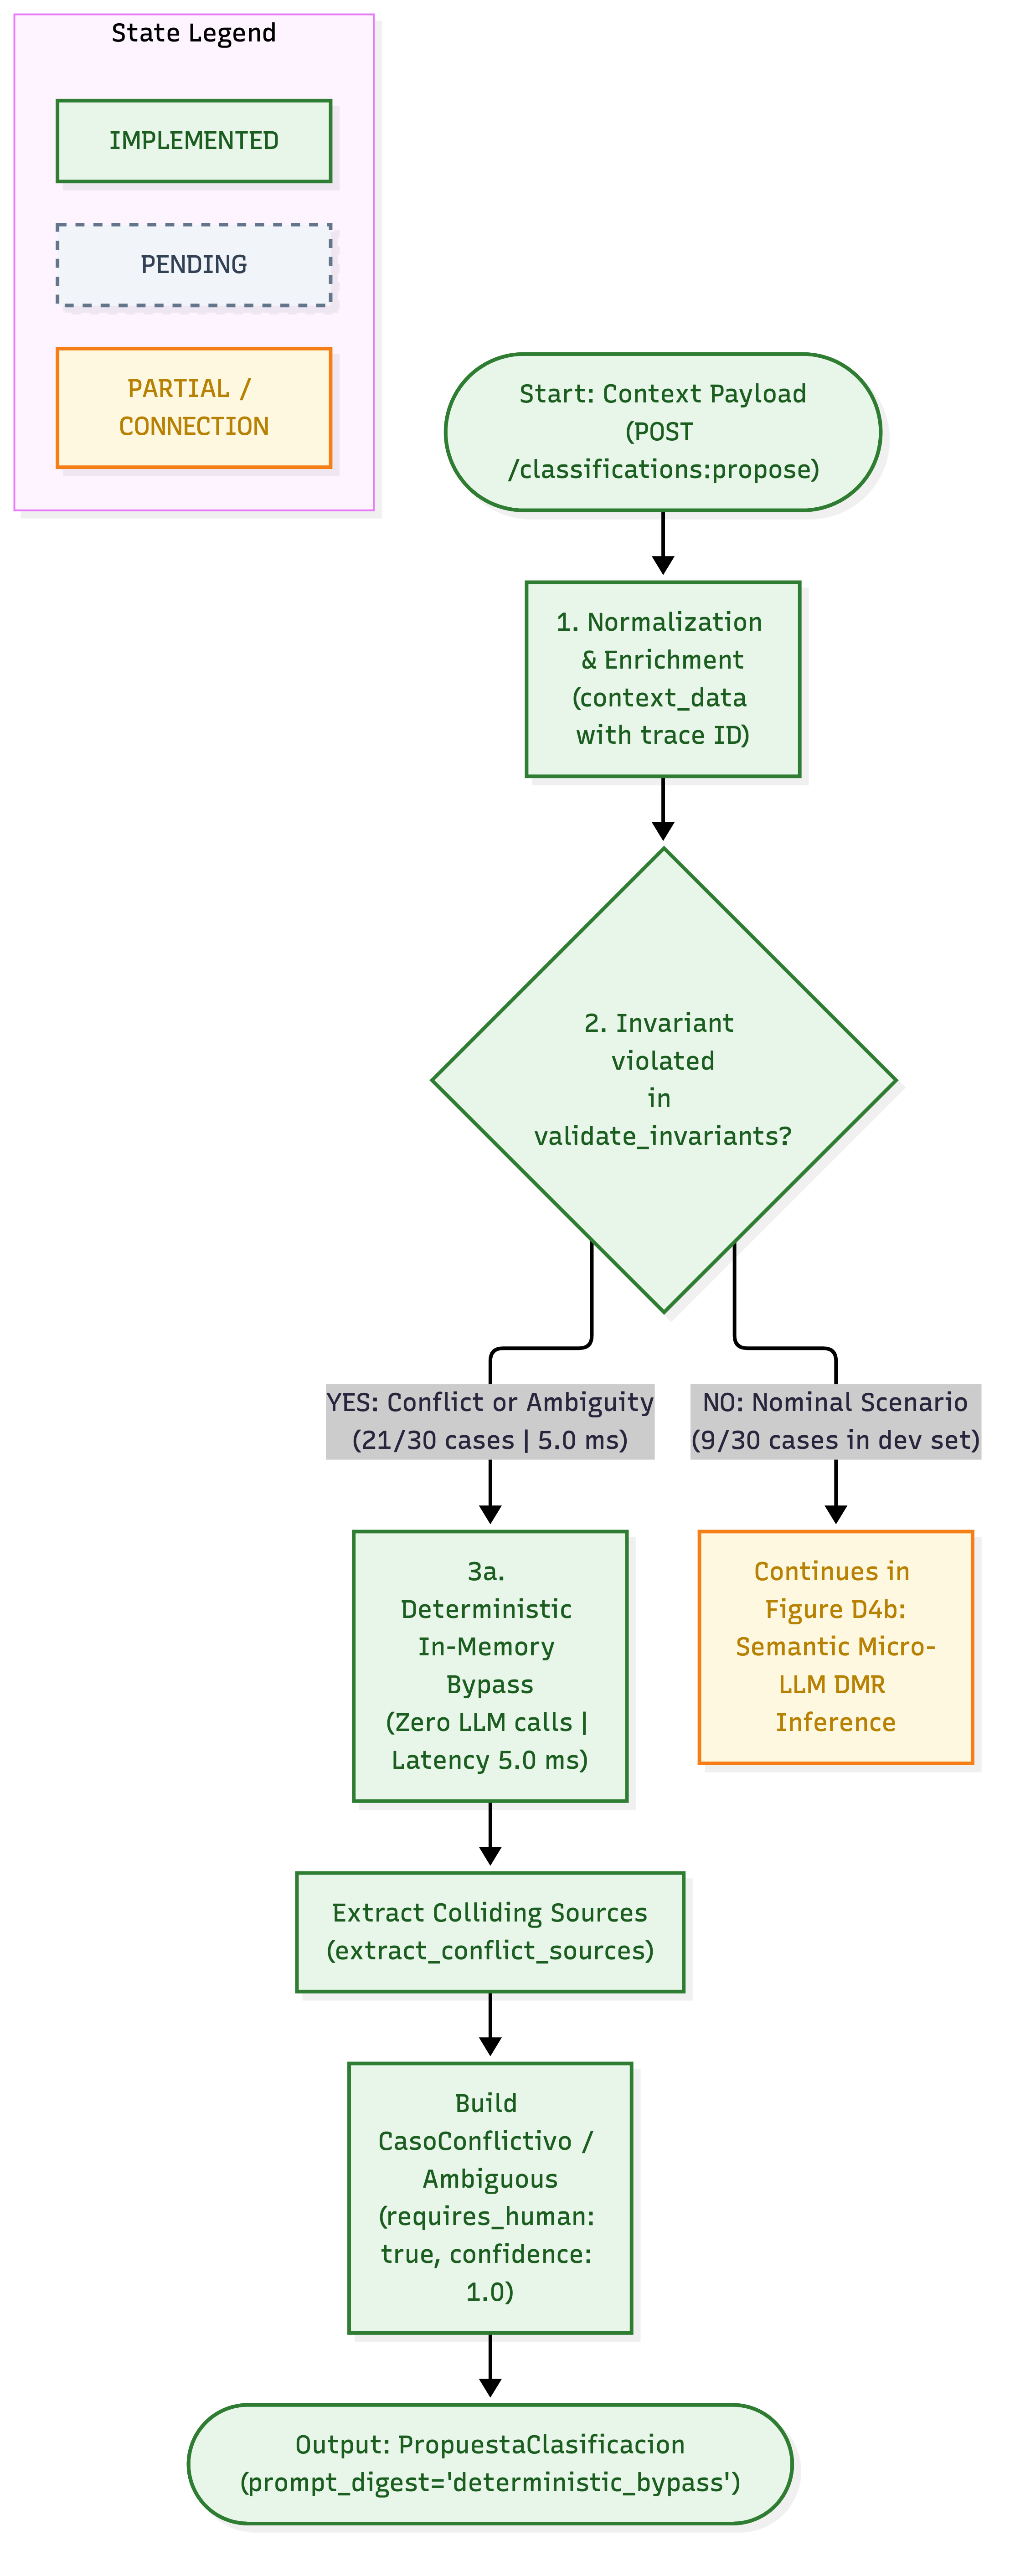
\includegraphics[width=0.88\textwidth,height=0.68\textheight,keepaspectratio]{docs/diagrams/out/d04a_classifier_flow_en.png}
    \caption{Figure D4a. Hybrid Intention Classifier Flow (Part 1: Ingestion, Normalization and Deterministic Bypass). Presents declarative request ingestion, contextual normalization, and in-memory invariant evaluation via deterministic hooks, resolving 70\% of dev set cases (21 of 30 cases) with 5.0~ms deterministic latency without invoking neural model. Connects to Node A (Figure D4b).}
    \label{fig:d04a_classifier_flow_en}
\end{figure}

% --- Figure D4b: Hybrid Classifier Flow (Part 2: Micro-LLM Inference and Pydantic V2 Validation) ---
\begin{figure}[htbp]
    \centering
    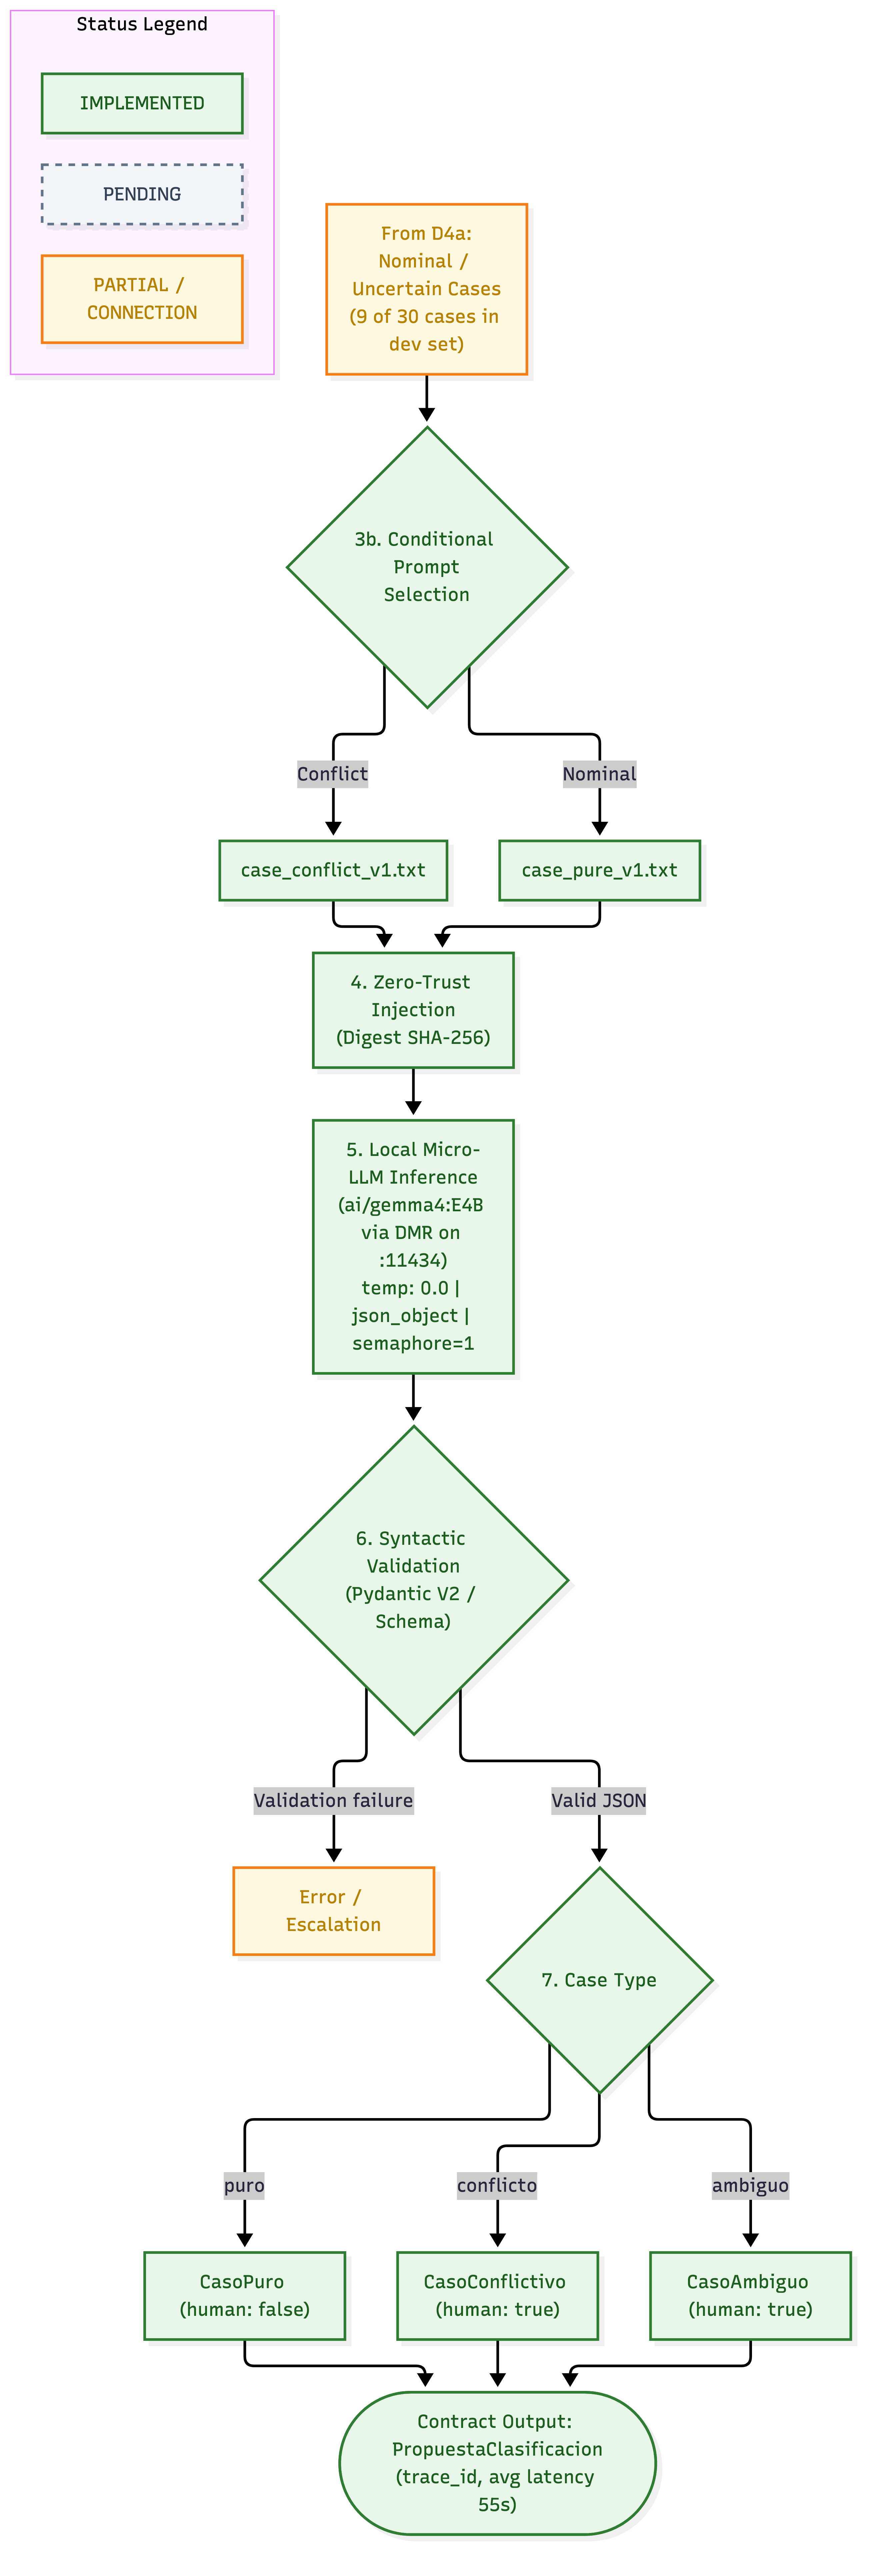
\includegraphics[width=0.88\textwidth,height=0.68\textheight,keepaspectratio]{docs/diagrams/out/d04b_classifier_flow_en.png}
    \caption{Figure D4b. Hybrid Intention Classifier Flow (Part 2: Micro-LLM Inference and Pydantic V2 Validation). Resumes from Node A (Figure D4a) for complex or ambiguous cases, illustrating conditional Zero-Trust prompt selection, local inference via DMR with \texttt{ai/gemma4:E4B} (9 cases, average latency 55,049.64~ms), syntactic/semantic validation, and final intention classification or human review routing.}
    \label{fig:d04b_classifier_flow_en}
\end{figure}

% --- Figure D6a: Operational Document State Flow (Part 1: Draft to Analyzed, Structuring and Blocking Routes) ---
\begin{figure}[htbp]
    \centering
    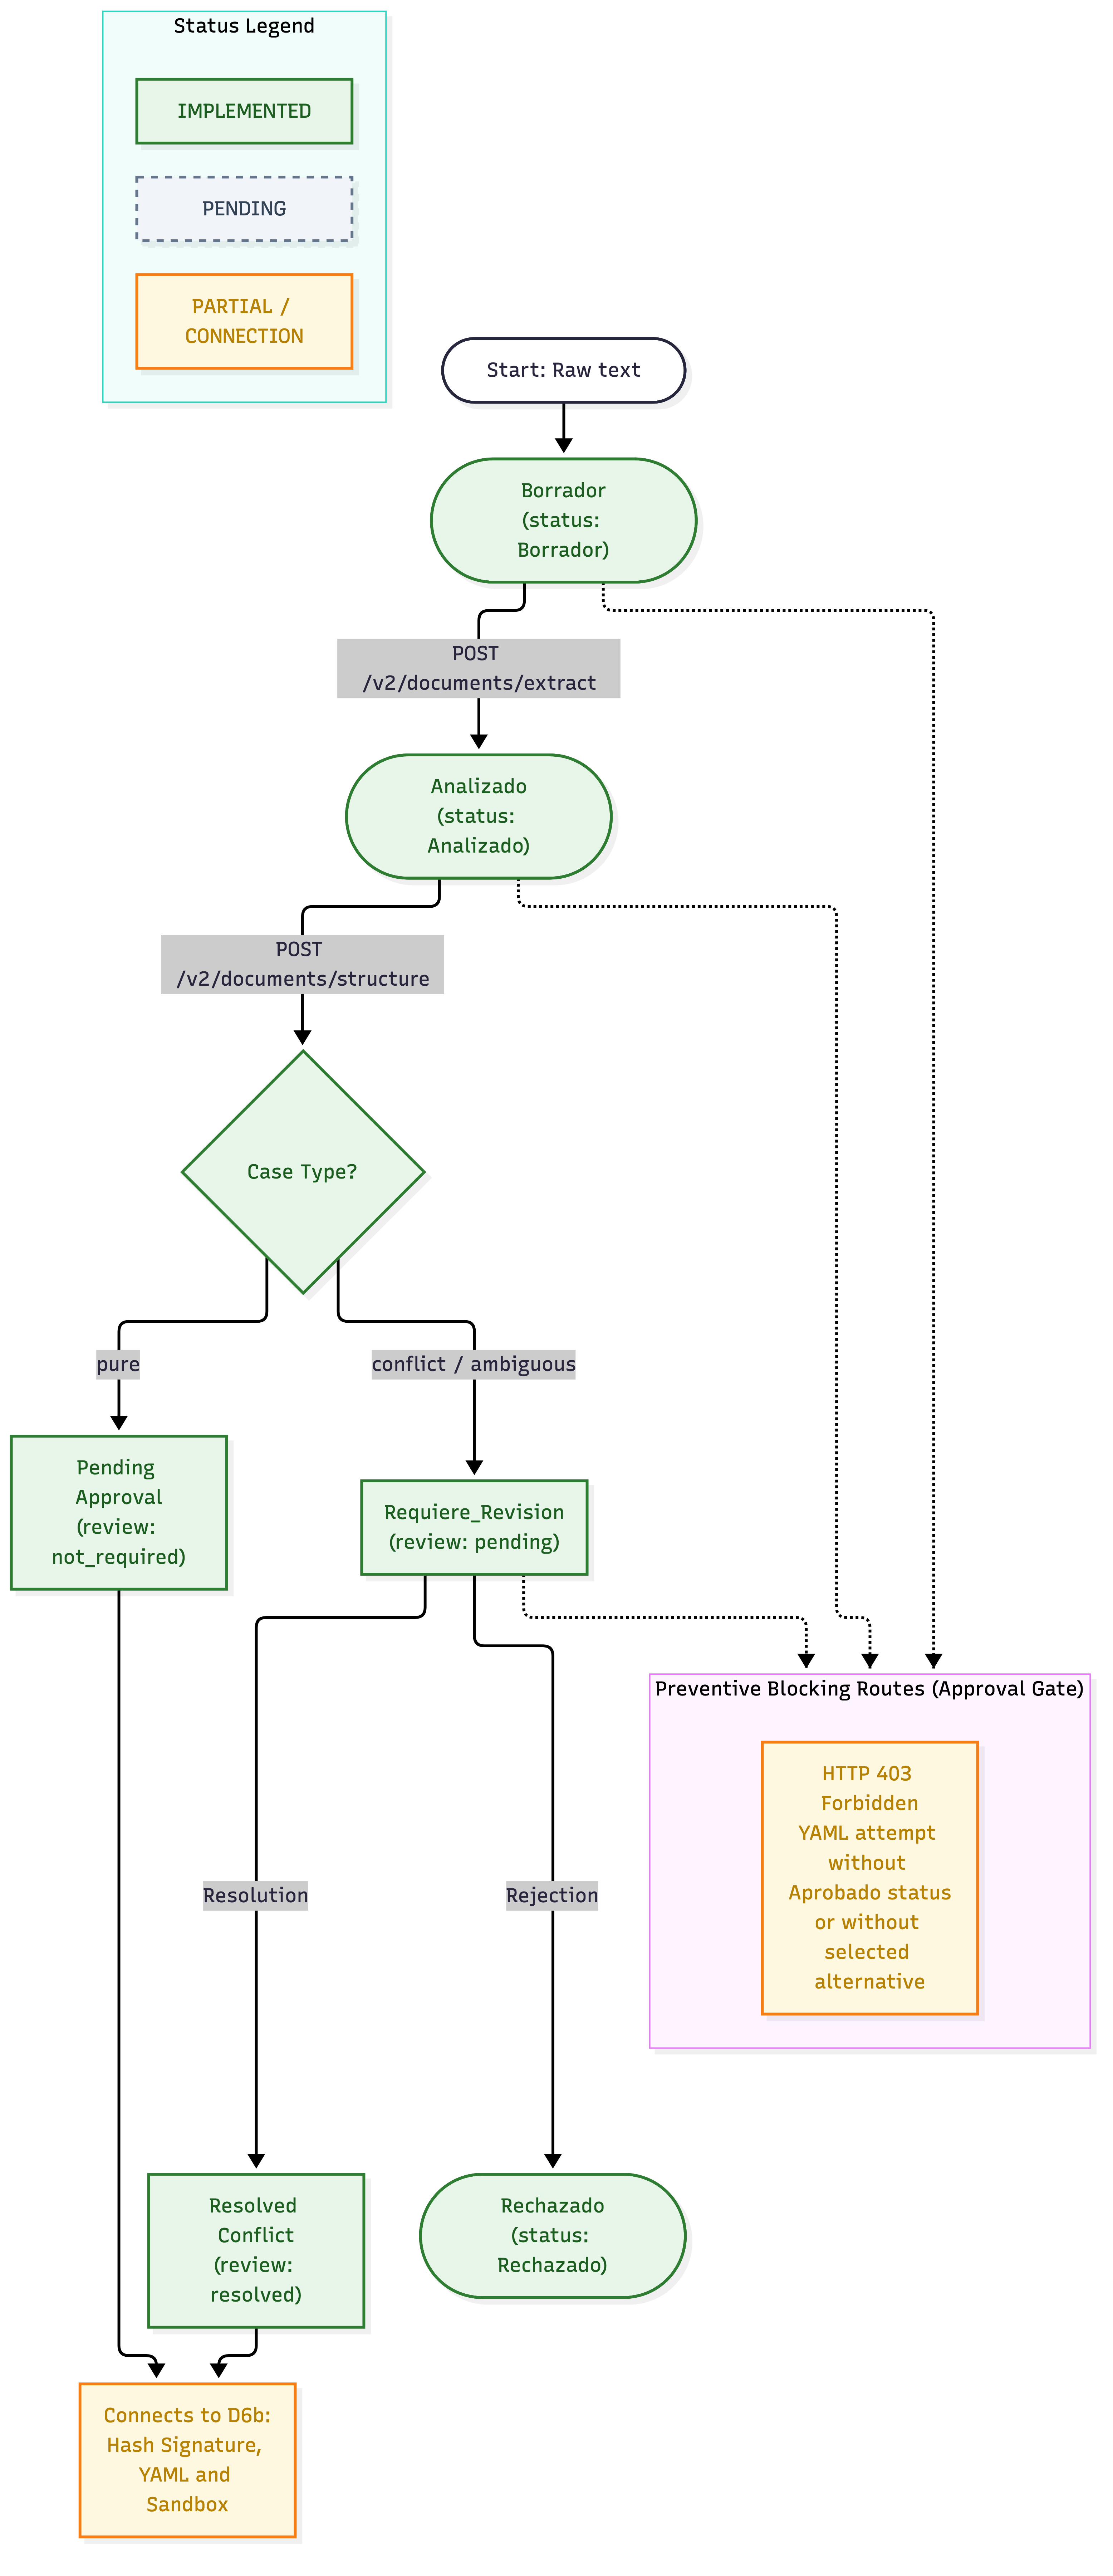
\includegraphics[width=0.88\textwidth,height=0.68\textheight,keepaspectratio]{docs/diagrams/out/d06a_document_lifecycle_en.png}
    \caption{Figure D6a. Operational Document State Flow (Part 1: Draft to Analyzed, Structuring and Blocking Routes). Models initial lifecycle from \texttt{Borrador} creation, structured analysis (\texttt{GoalSpecArtifact}, \texttt{PlanSpecArtifact}), and branching toward \texttt{Requiere\_Revision}, \texttt{Rechazado}, or \texttt{Analizado}. Shows security gates blocking invalid schemas or contradictory intentions. Connects to Approval Checkpoint (Figure D6b).}
    \label{fig:d06a_document_lifecycle_en}
\end{figure}

% --- Figure D6b: Operational Document State Flow (Part 2: Approval, Canonical Hash and Sandbox Installation) ---
\begin{figure}[htbp]
    \centering
    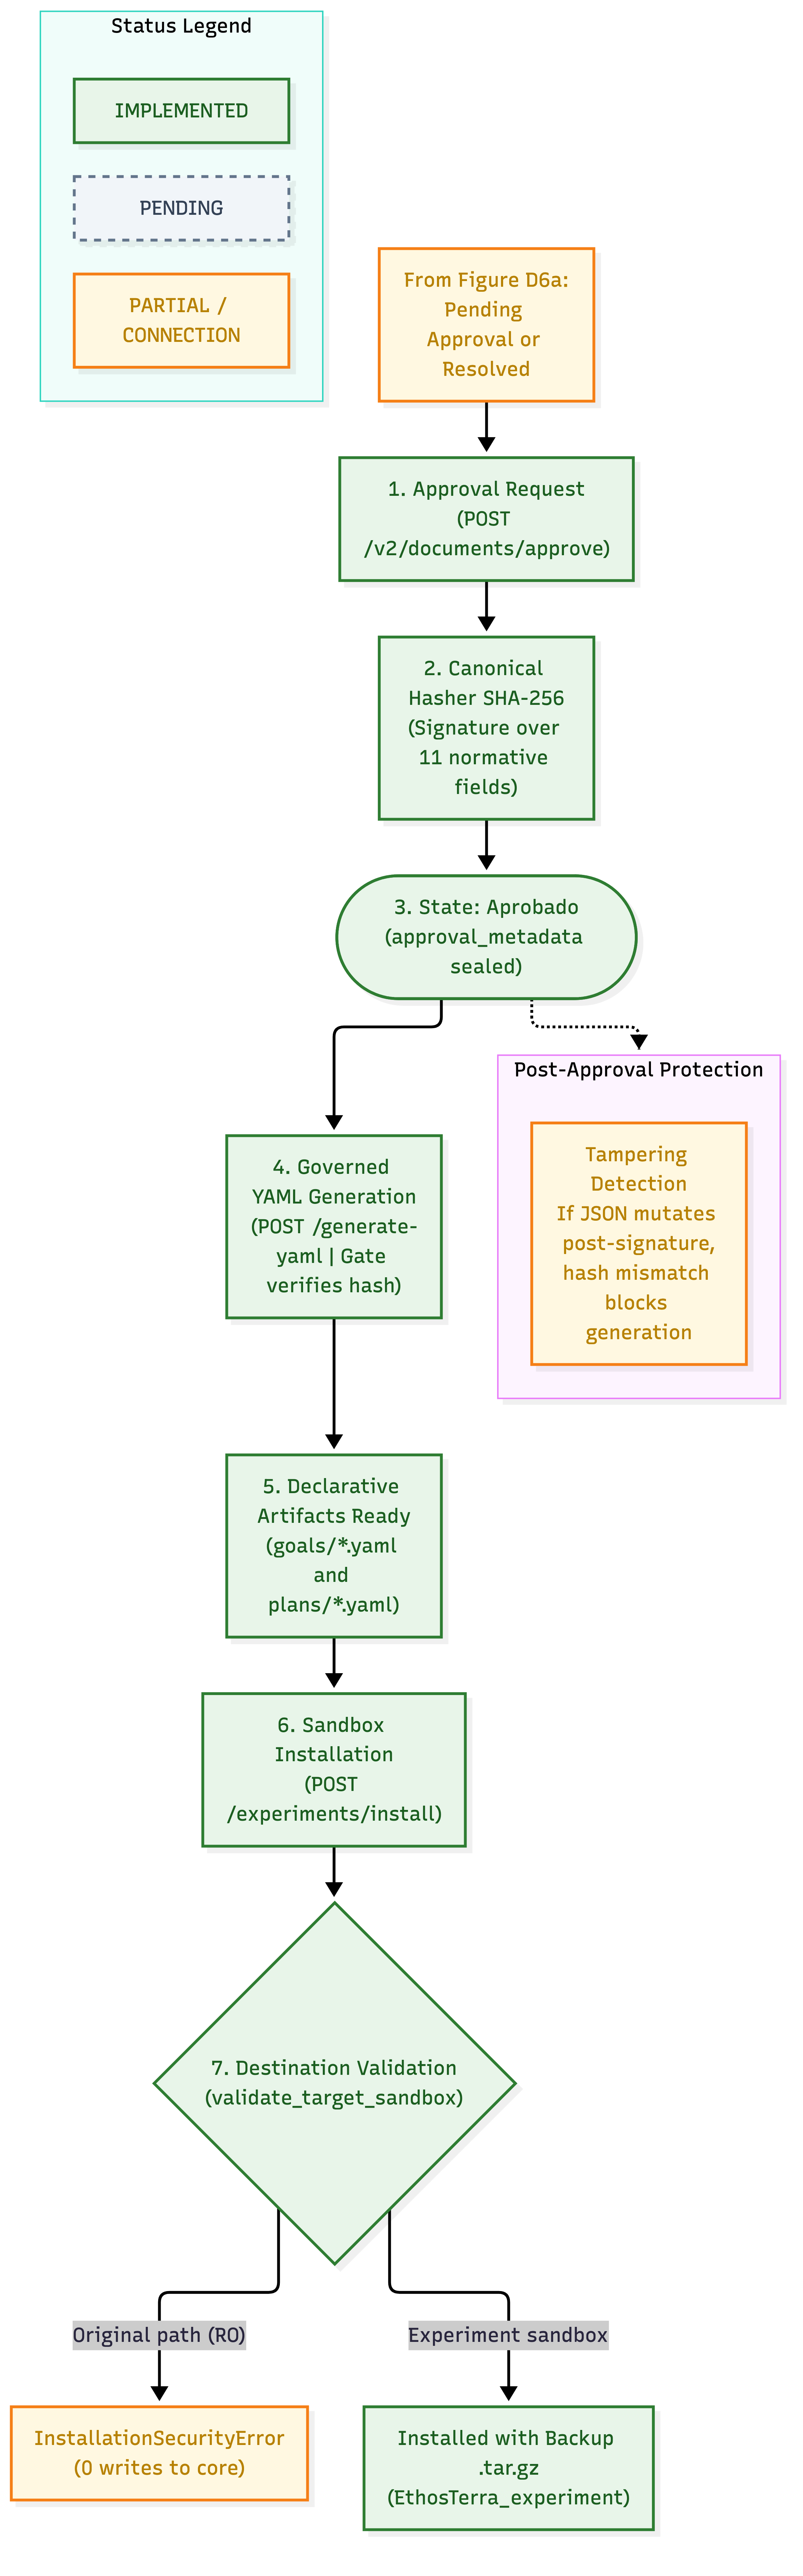
\includegraphics[width=0.88\textwidth,height=0.68\textheight,keepaspectratio]{docs/diagrams/out/d06b_document_lifecycle_en.png}
    \caption{Figure D6b. Operational Document State Flow (Part 2: Approval, Canonical Hash and Sandbox Installation). Resumes from \texttt{Analizado} (Figure D6a), detailing transition to \texttt{Aprobado} via human signing with 11-field SHA-256 canonical hash, confined YAML generation, installation with compressed backup (.tar.gz), and immediate HTTP 403 blocking or atomic rollback upon tampering.}
    \label{fig:d06b_document_lifecycle_en}
\end{figure}

% --- Figure D11: Status Map and Development Roadmap ---
\begin{figure}[htbp]
    \centering
    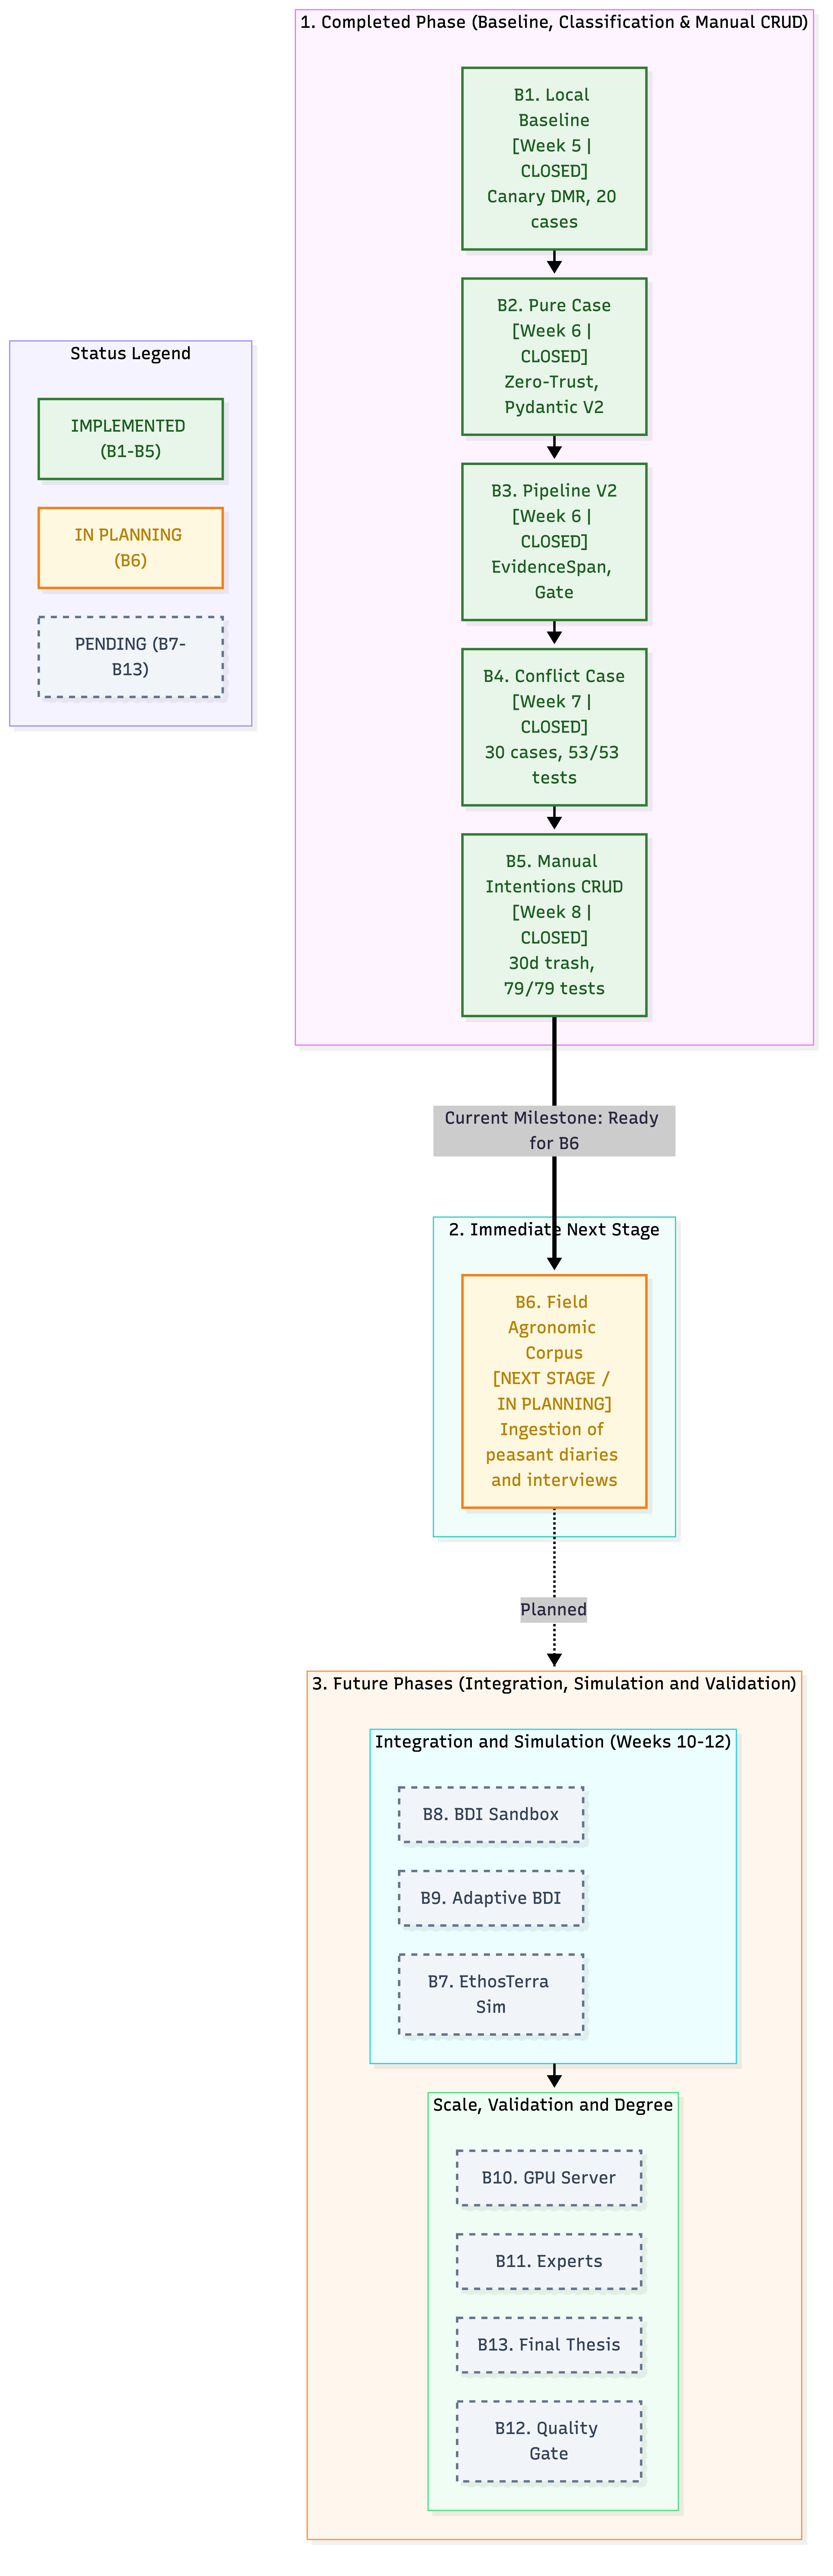
\includegraphics[width=0.88\textwidth,height=0.68\textheight,keepaspectratio]{docs/diagrams/out/d11_status_roadmap_en.png}
    \caption{Figure D11. Status Map and Development Roadmap (Blocks B1 to B13). Visualizes the consolidated progress of closed blocks (B1--B5, with 79/79 passed tests), the immediate position of next increment (B6: Field agronomic corpus), and subsequent integration and validation phases (B7--B13).}
    \label{fig:d11_status_roadmap_en}
\end{figure}


\clearpage

% ==============================================================================
% SECTION 4: FIGURES IN ENGLISH — METHODOLOGICAL APPENDIX
% ==============================================================================

% --- Figure D2: System Context (C4 Level 1) ---
\begin{figure}[htbp]
    \centering
    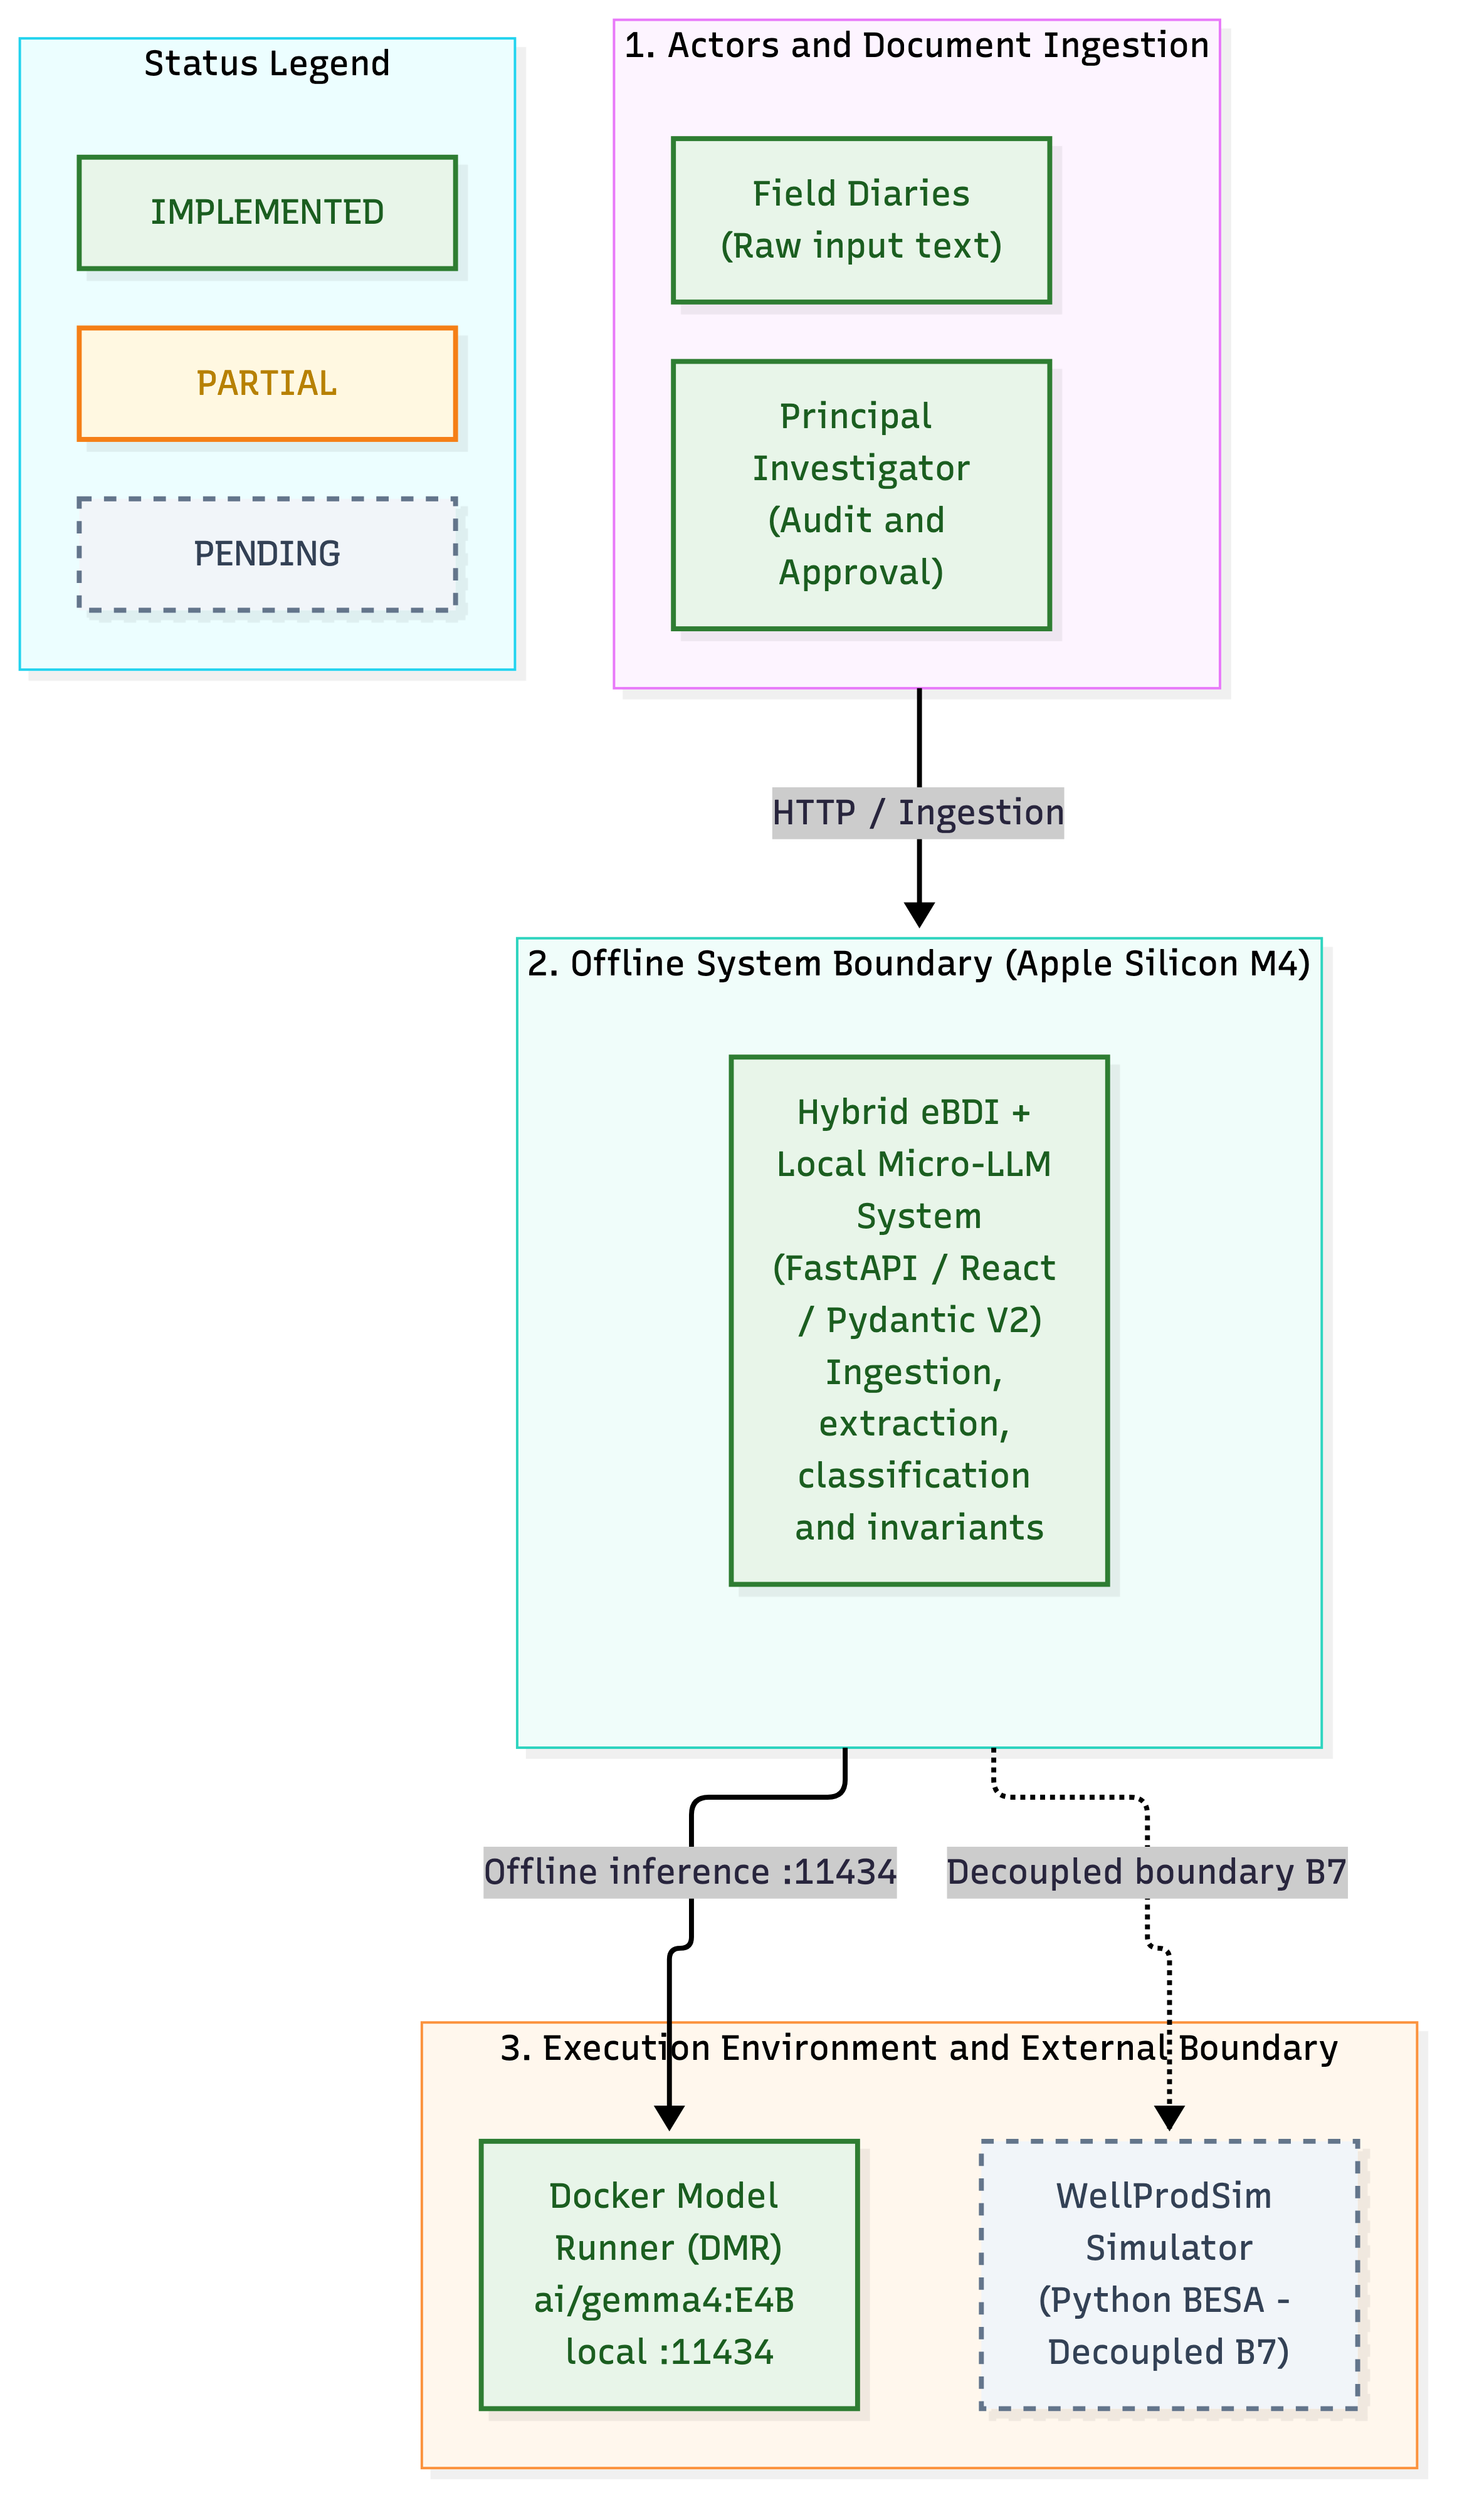
\includegraphics[width=0.88\textwidth,height=0.68\textheight,keepaspectratio]{docs/diagrams/out/d02_c4_context_en.png}
    \caption{Figure D2. System Context Diagram (C4 Level 1). Demarcates human actors (principal investigator and reviewing directors), field documentary sources, Docker Model Runner inference runtime, and the 100\% offline execution boundary on Apple Silicon M4 hardware.}
    \label{fig:d02_c4_context_en}
\end{figure}

% --- Figure D3: Backend Components (C4 Level 3) ---
\begin{figure}[htbp]
    \centering
    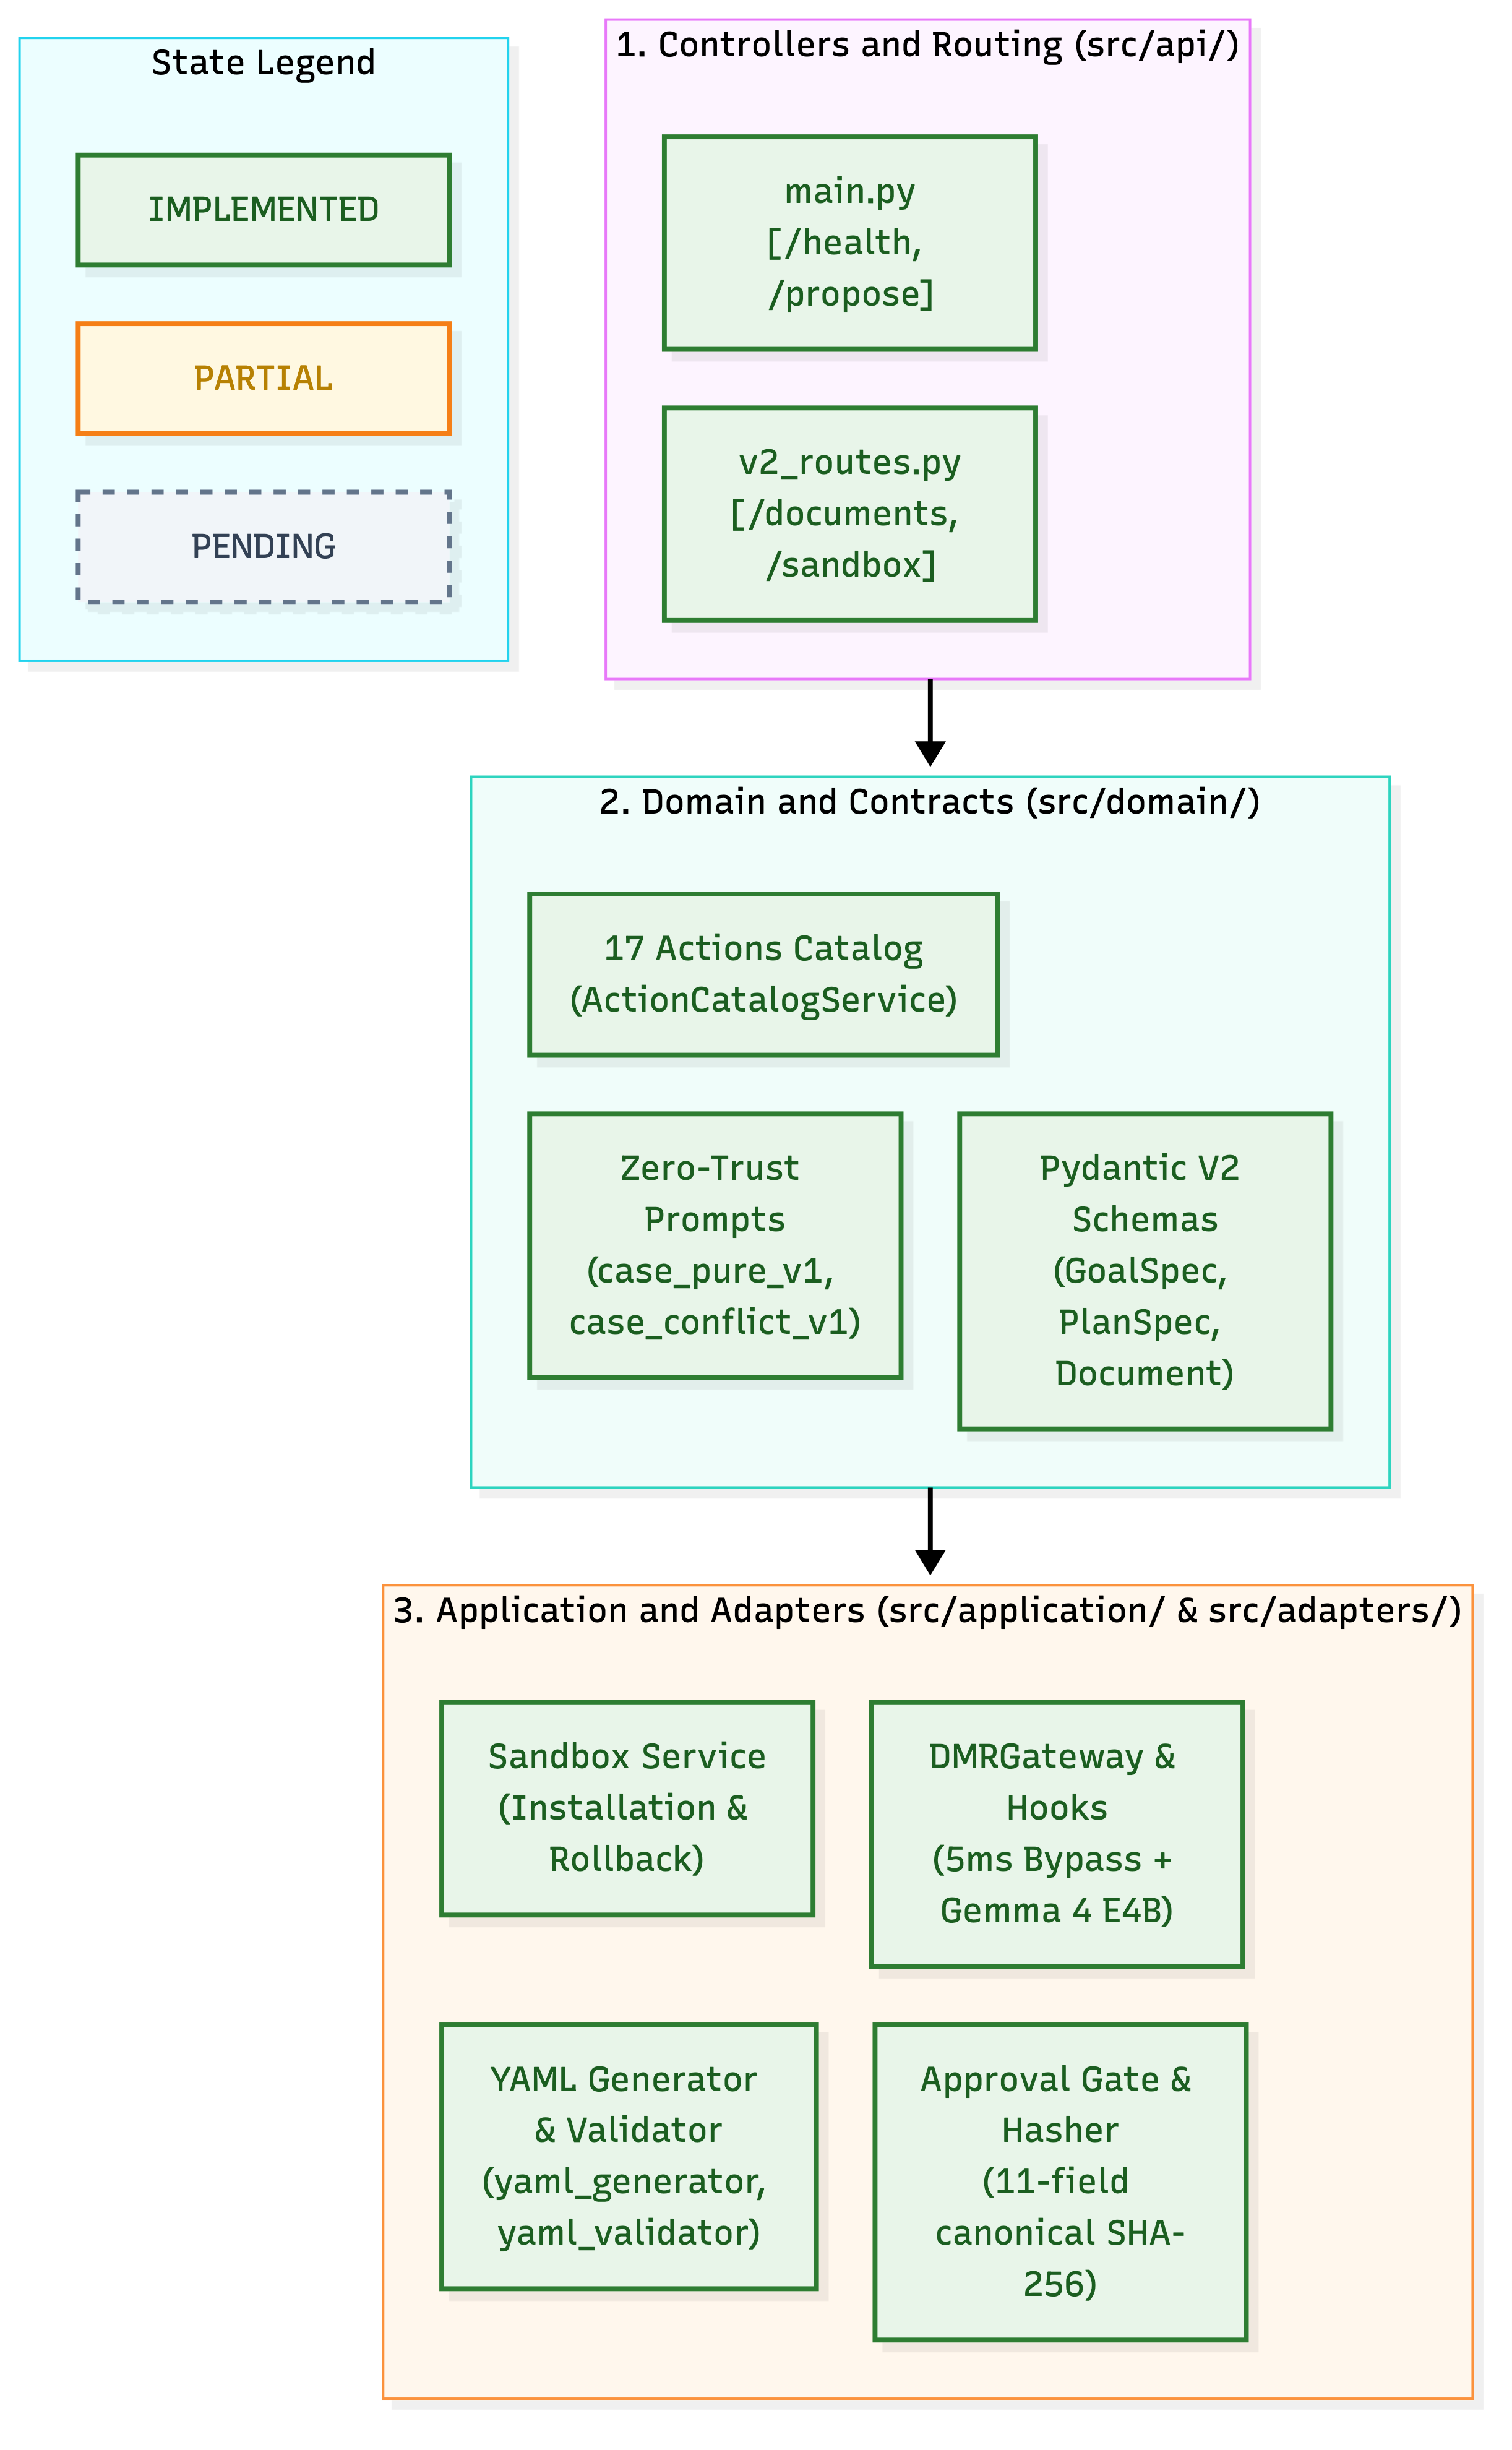
\includegraphics[width=0.88\textwidth,height=0.68\textheight,keepaspectratio]{docs/diagrams/out/d03_c4_components_en.png}
    \caption{Figure D3. Internal Backend Components (C4 Level 3). Specifies the modular organization in \texttt{apps/api/src/}: routers, Pydantic V2 schemas, verified catalog of 17 EthosTerra formal actions, 11-field SHA-256 canonical hasher, and sandbox services.}
    \label{fig:d03_c4_components_en}
\end{figure}

% --- Figure D5a: Conflict Case Flow (Part 1: Collision Detection and Source Traceability) ---
\begin{figure}[htbp]
    \centering
    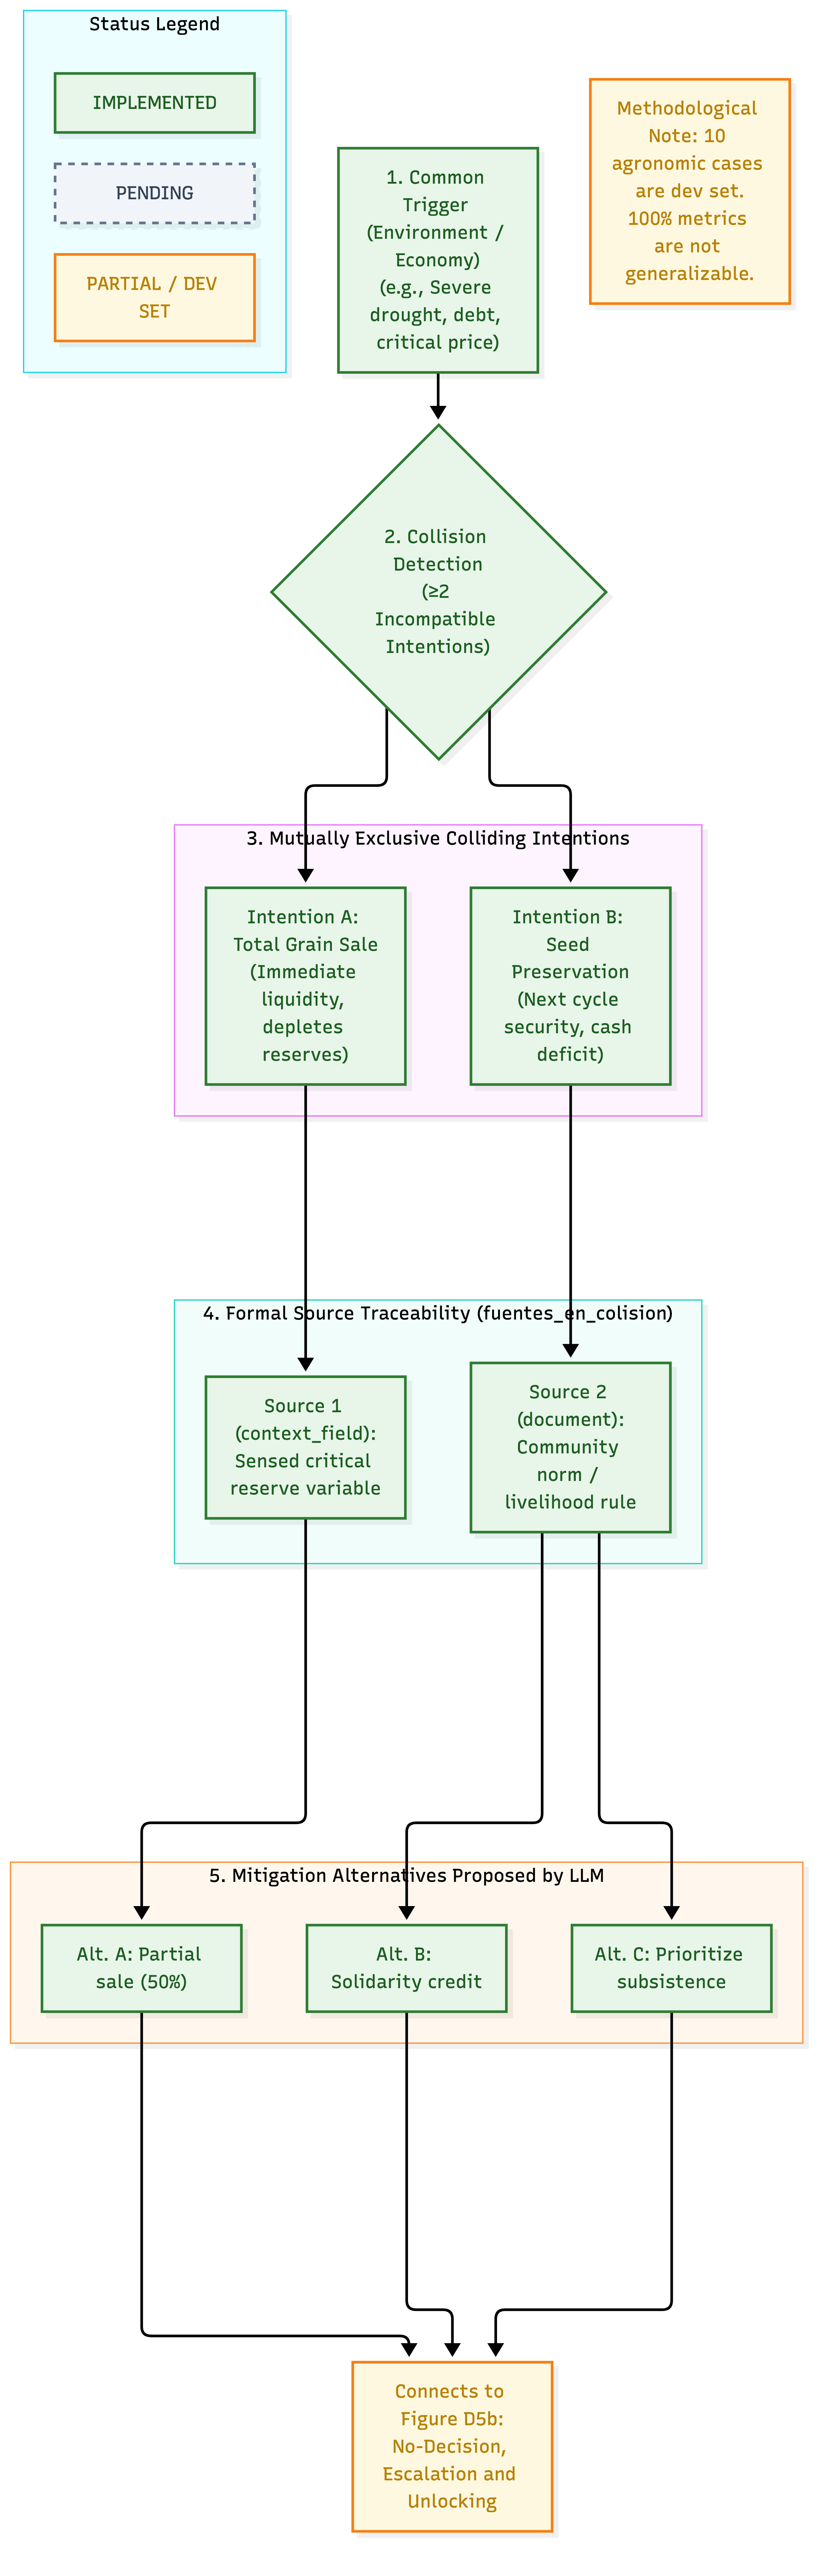
\includegraphics[width=0.88\textwidth,height=0.68\textheight,keepaspectratio]{docs/diagrams/out/d05a_conflict_flow_en.png}
    \caption{Figure D5a. Conflict Case Flow (Part 1: Collision Detection and Source Traceability). Details collision identification between contradictory agronomic intentions given a common trigger, and forensic origin mapping (\texttt{context\_field} vs. \texttt{document}). Connects to Node B (Figure D5b).}
    \label{fig:d05a_conflict_flow_en}
\end{figure}

% --- Figure D5b: Conflict Case Flow (Part 2: Alternatives Proposal and Human Escalation) ---
\begin{figure}[htbp]
    \centering
    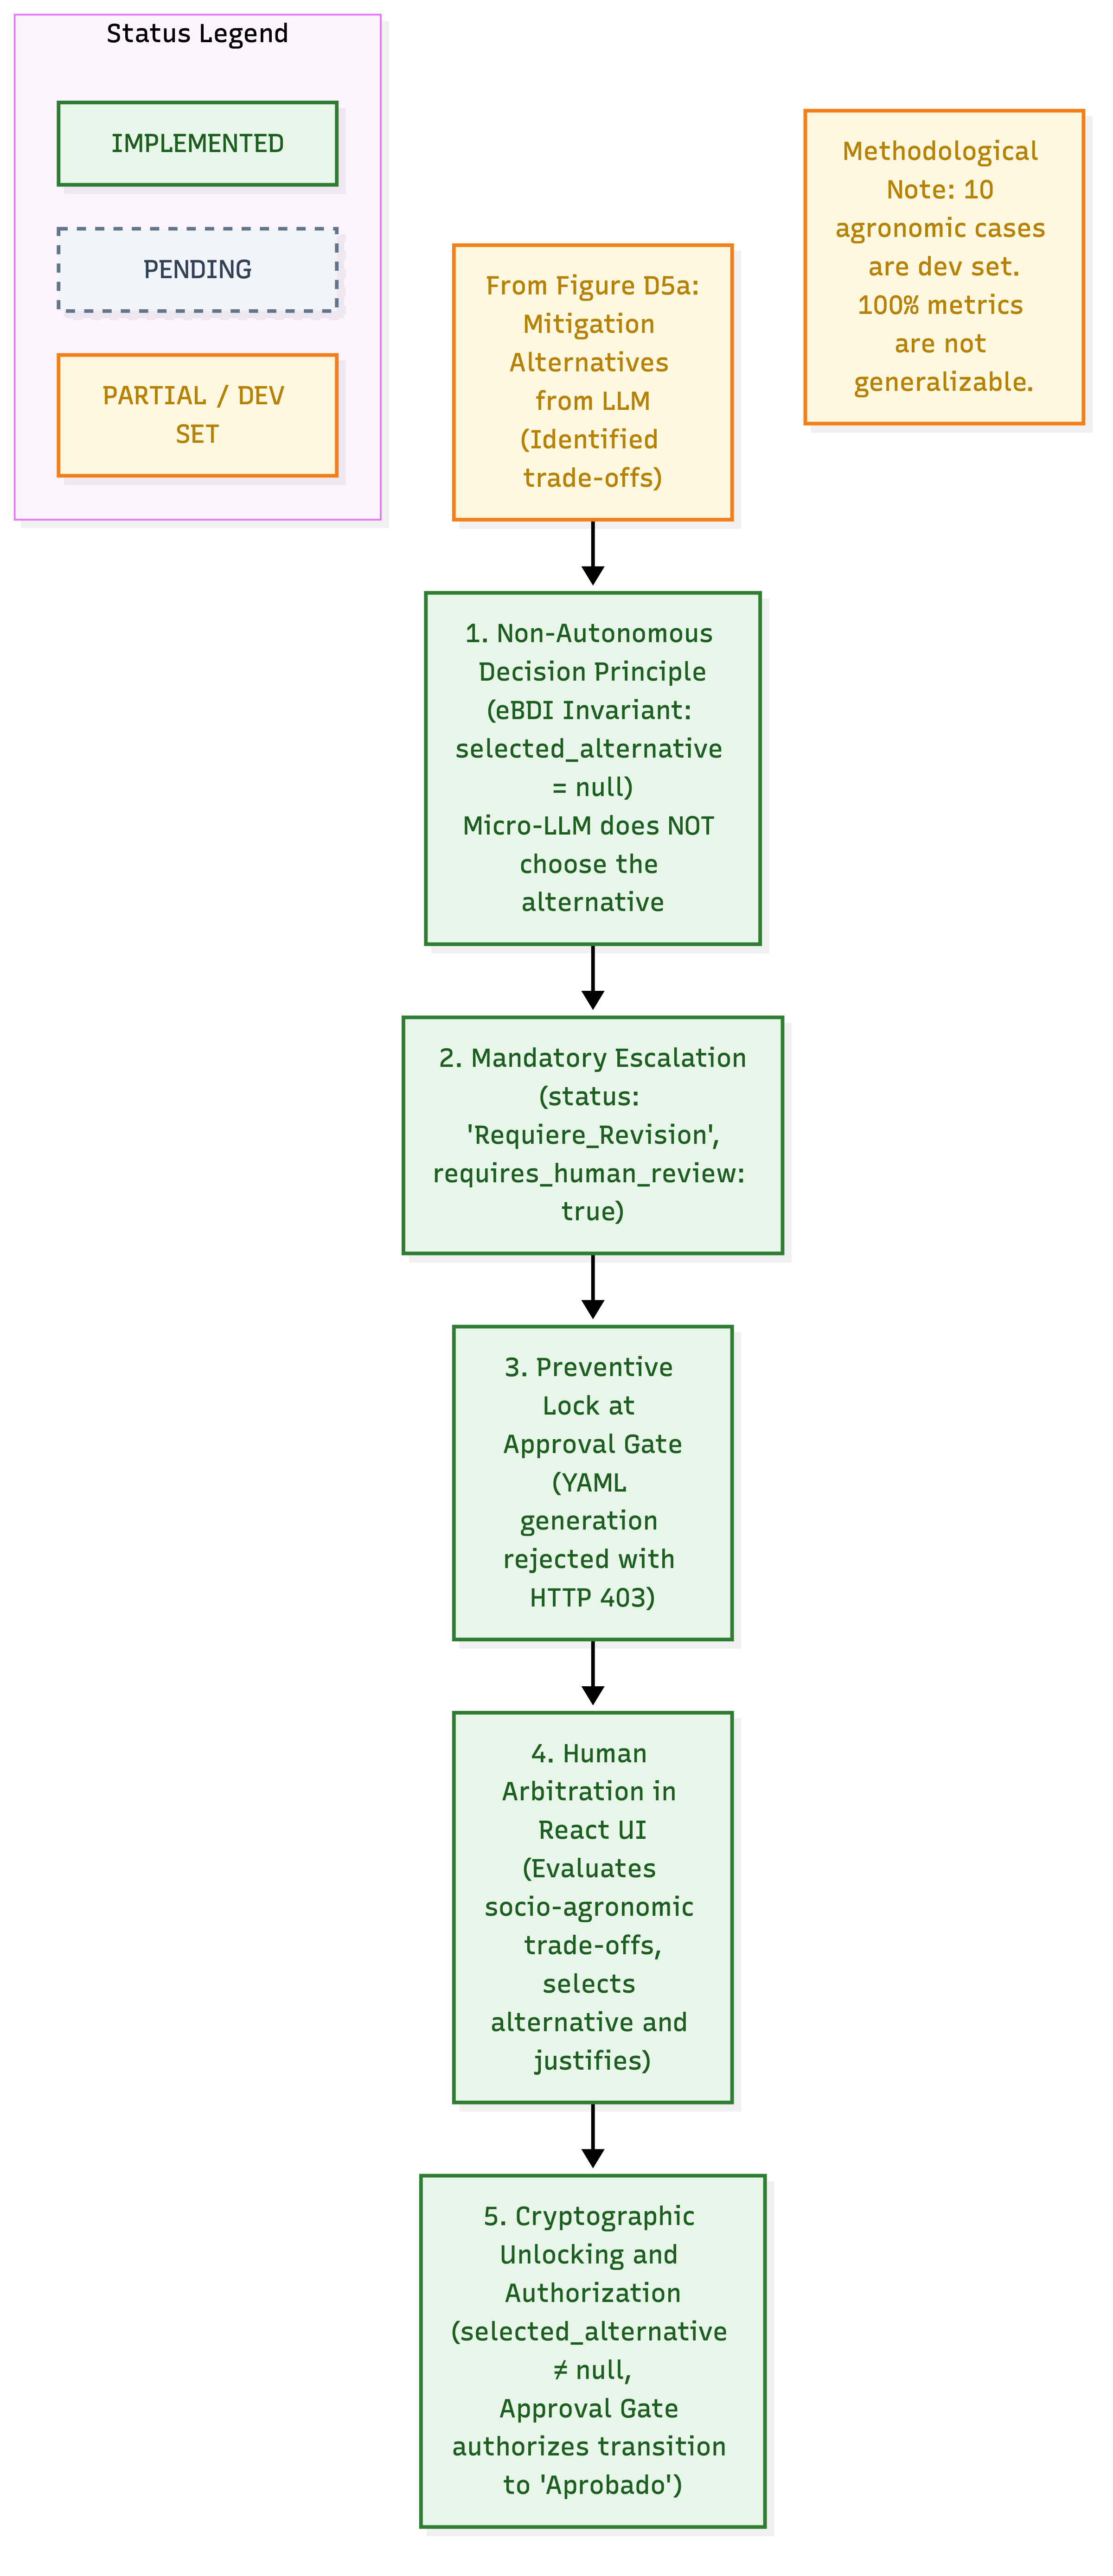
\includegraphics[width=0.88\textwidth,height=0.68\textheight,keepaspectratio]{docs/diagrams/out/d05b_conflict_flow_en.png}
    \caption{Figure D5b. Conflict Case Flow (Part 2: Alternatives Proposal and Human Escalation). Resumes from Node B (Figure D5a), illustrating structured mitigation alternatives proposal (A/B/C), the inviolable autonomous non-decision principle (\texttt{selected\_alternative = null}), and mandatory escalation to human arbitration.}
    \label{fig:d05b_conflict_flow_en}
\end{figure}

% --- Figure D7: Approval Gate Sequence (Landscape Page) ---
\begin{landscape}
\begin{figure}[htbp]
    \centering
    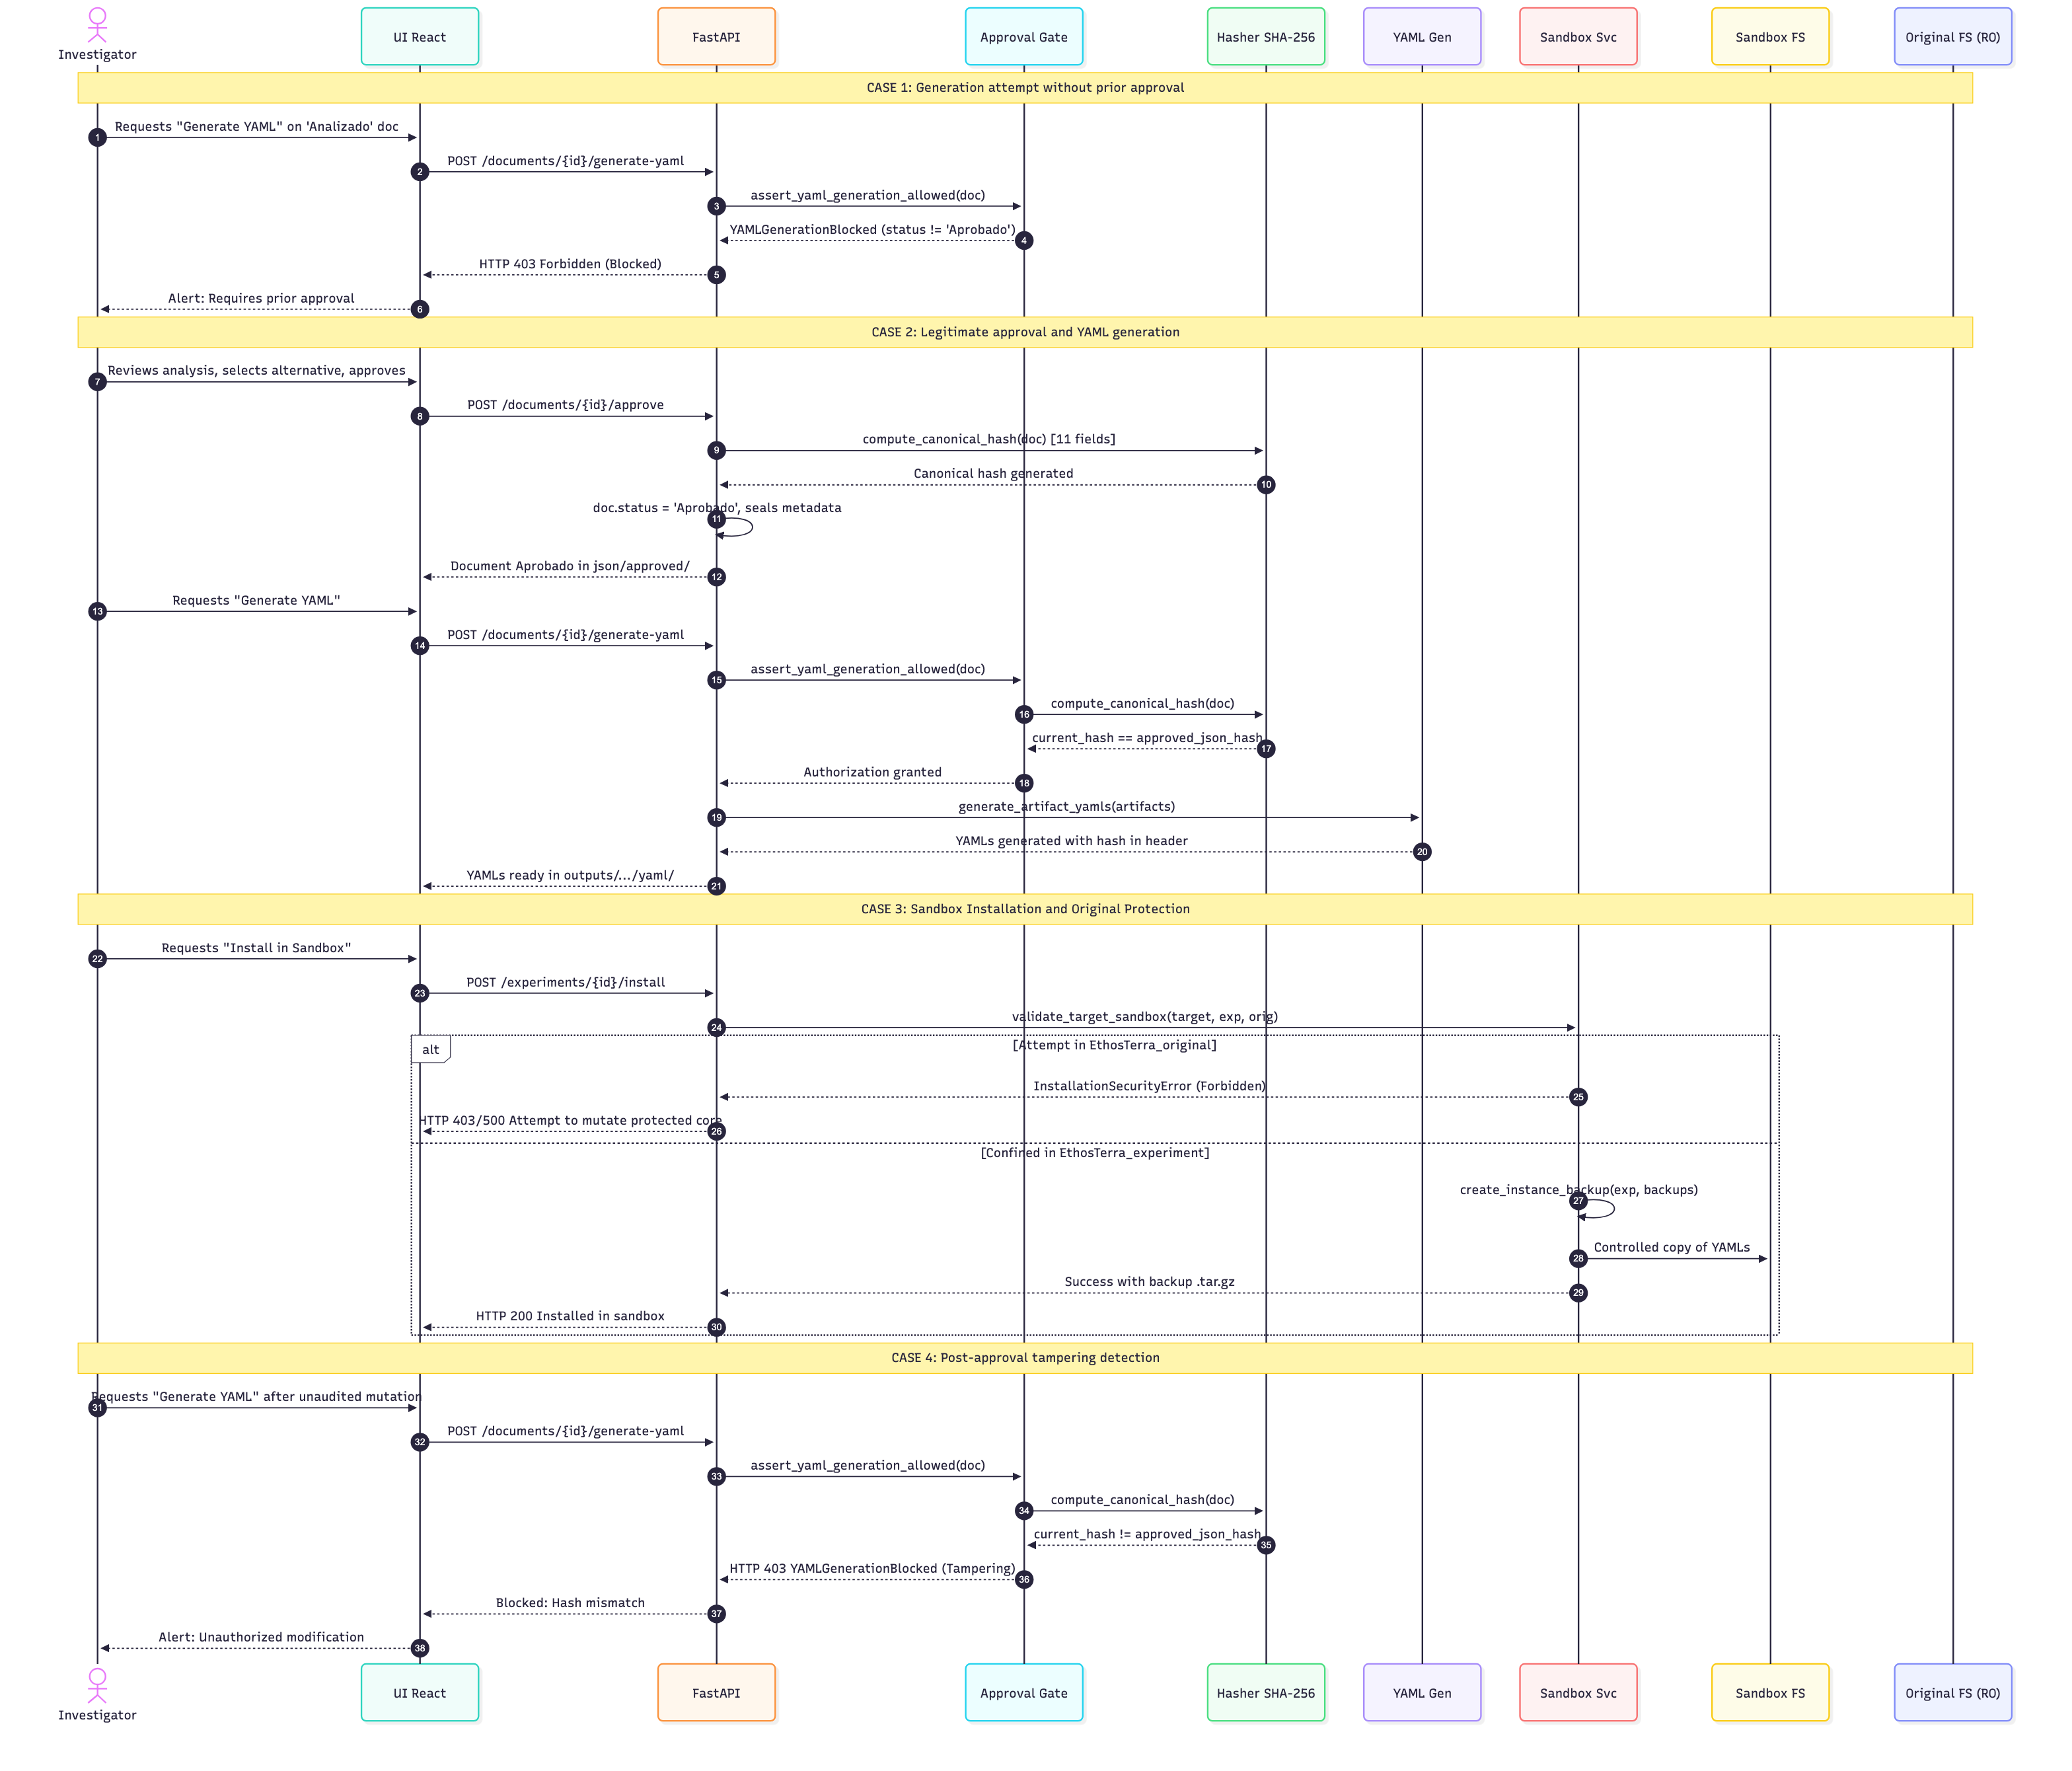
\includegraphics[width=0.95\linewidth,height=0.82\textheight,keepaspectratio]{docs/diagrams/out/d07_approval_gate_seq_en.png}
    \caption{Figure D7. Approval Gate, Security Gates and Sandbox Sequence. Details temporal interactions between investigator, UI, API, and application services across 5 scenarios: unauthorized block (403), legitimate canonical signing, sandbox installation with .tar.gz backup, tampering detection, and atomic rollback.}
    \label{fig:d07_approval_gate_seq_en}
\end{figure}
\end{landscape}

% --- Figure D8: Data Model and Contracts (Landscape Page) ---
\begin{landscape}
\begin{figure}[htbp]
    \centering
    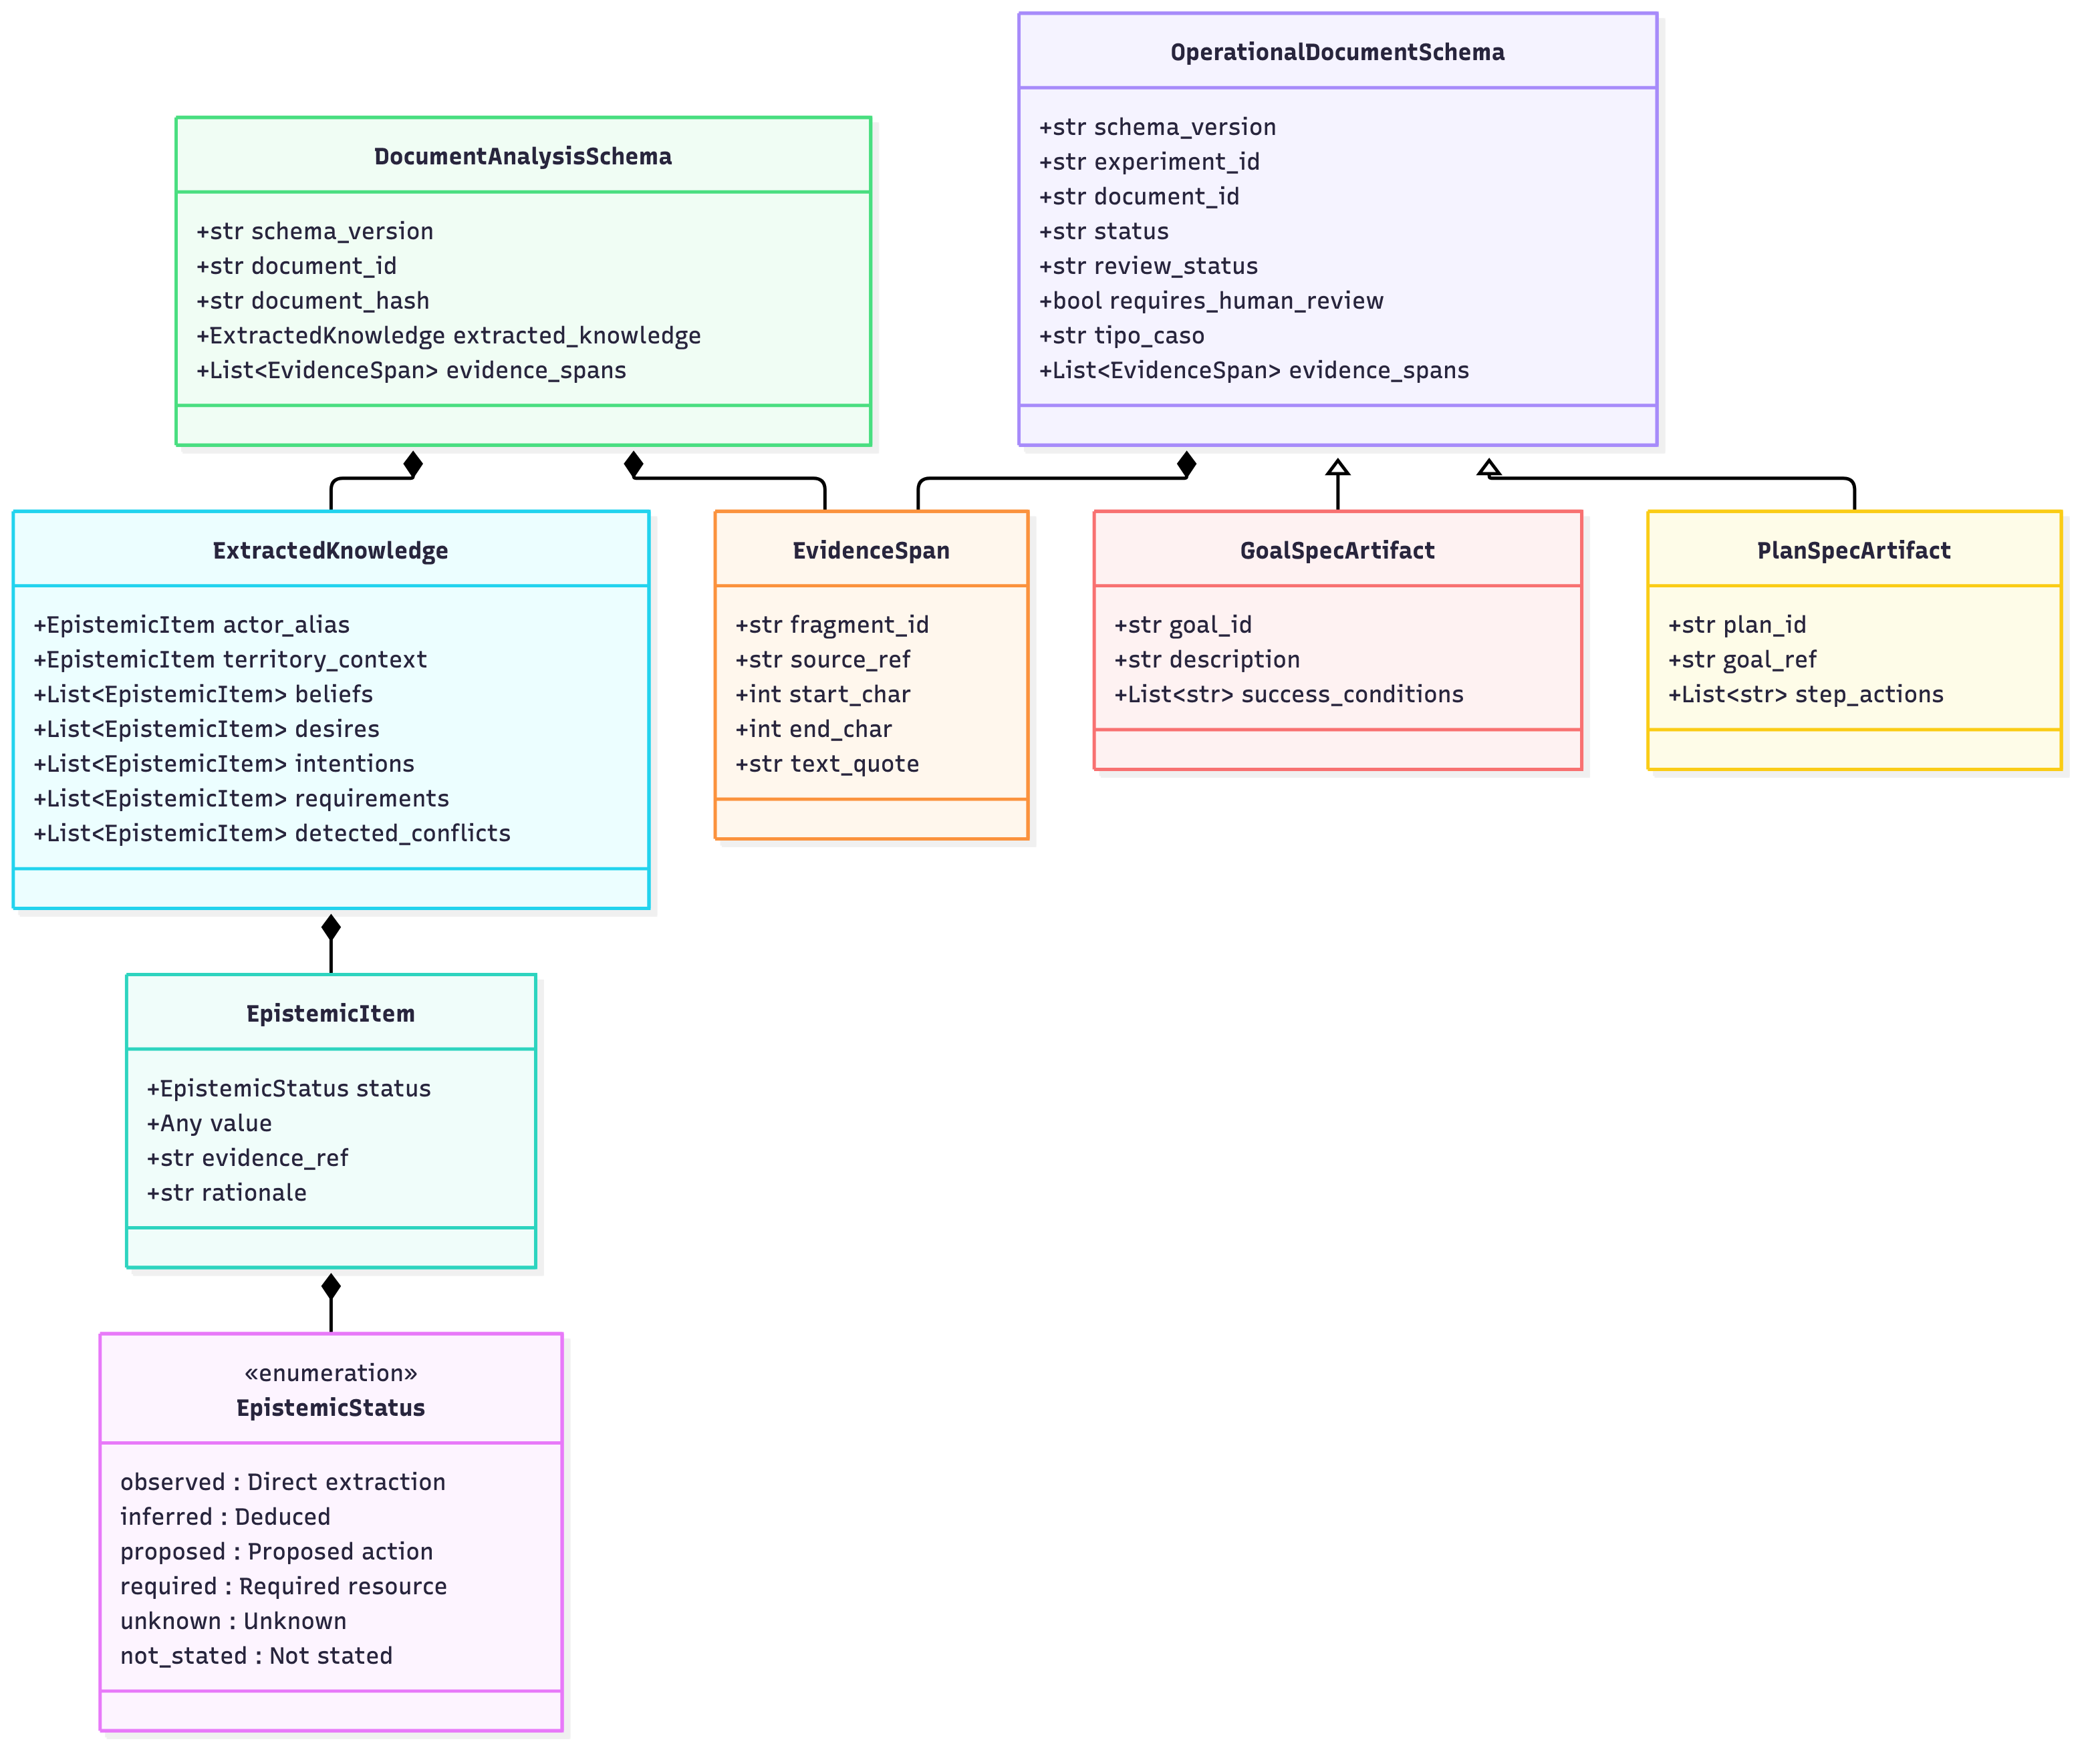
\includegraphics[width=0.95\linewidth,height=0.82\textheight,keepaspectratio]{docs/diagrams/out/d08_data_model_contracts_en.png}
    \caption{Figure D8. Class Diagram of Data Model and Pydantic V2 Contracts. Models declarative entities \texttt{GoalSpecArtifact}, \texttt{PlanSpecArtifact}, \texttt{OperationalDocumentSchema}, the 6 epistemic states (\texttt{observed}, \texttt{inferred}, \texttt{proposed}, \texttt{required}, \texttt{unknown}, \texttt{not\_stated}), and evidence spans (\texttt{EvidenceSpan}).}
    \label{fig:d08_data_model_contracts_en}
\end{figure}
\end{landscape}

% --- Figure D9a: Deployment and Environment (Part 1: Process Architecture and Local Ports) ---
\begin{figure}[htbp]
    \centering
    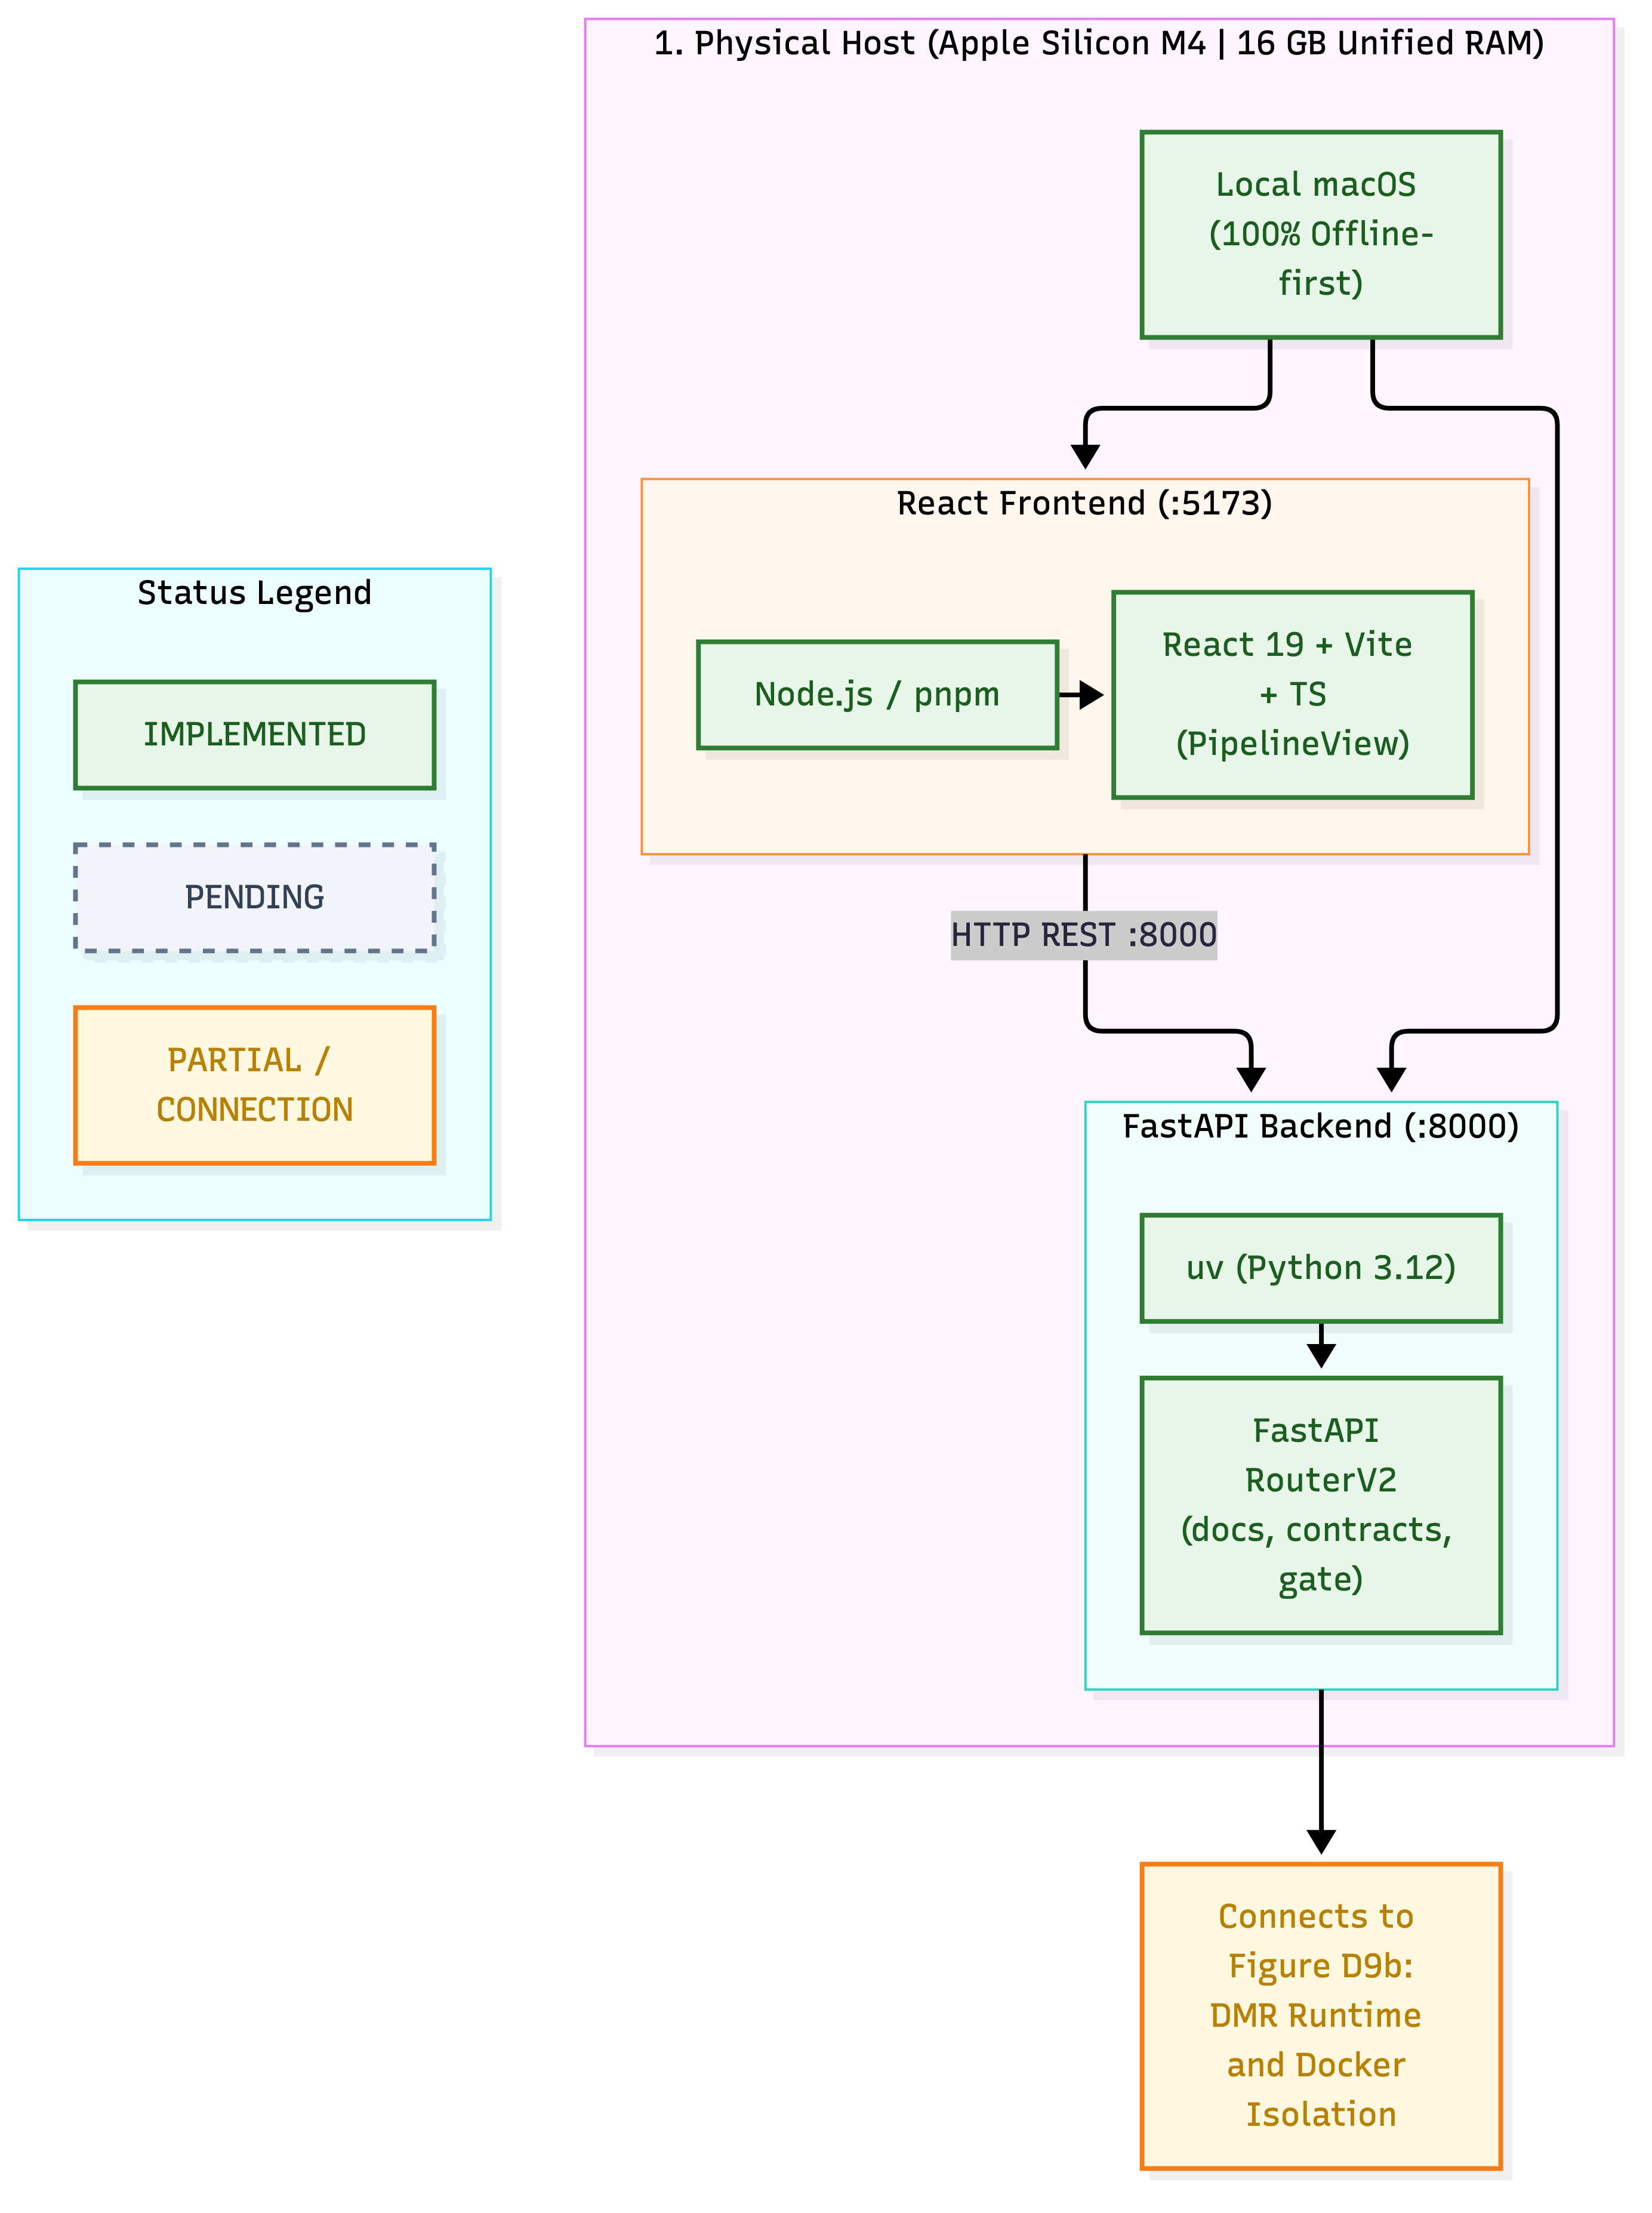
\includegraphics[width=0.88\textwidth,height=0.68\textheight,keepaspectratio]{docs/diagrams/out/d09a_deployment_env_en.png}
    \caption{Figure D9a. Deployment and Execution Environment (Part 1: Process Architecture and Local Ports). Details service topology on local physical workstation, specifying runtimes (Python 3.14 uv, Node.js pnpm) and internal communication ports (\texttt{:5173}, \texttt{:8000}, \texttt{:11434}). Connects to DMR runtime (Figure D9b).}
    \label{fig:d09a_deployment_env_en}
\end{figure}

% --- Figure D9b: Deployment and Environment (Part 2: DMR Containerization and Hardware Resources) ---
\begin{figure}[htbp]
    \centering
    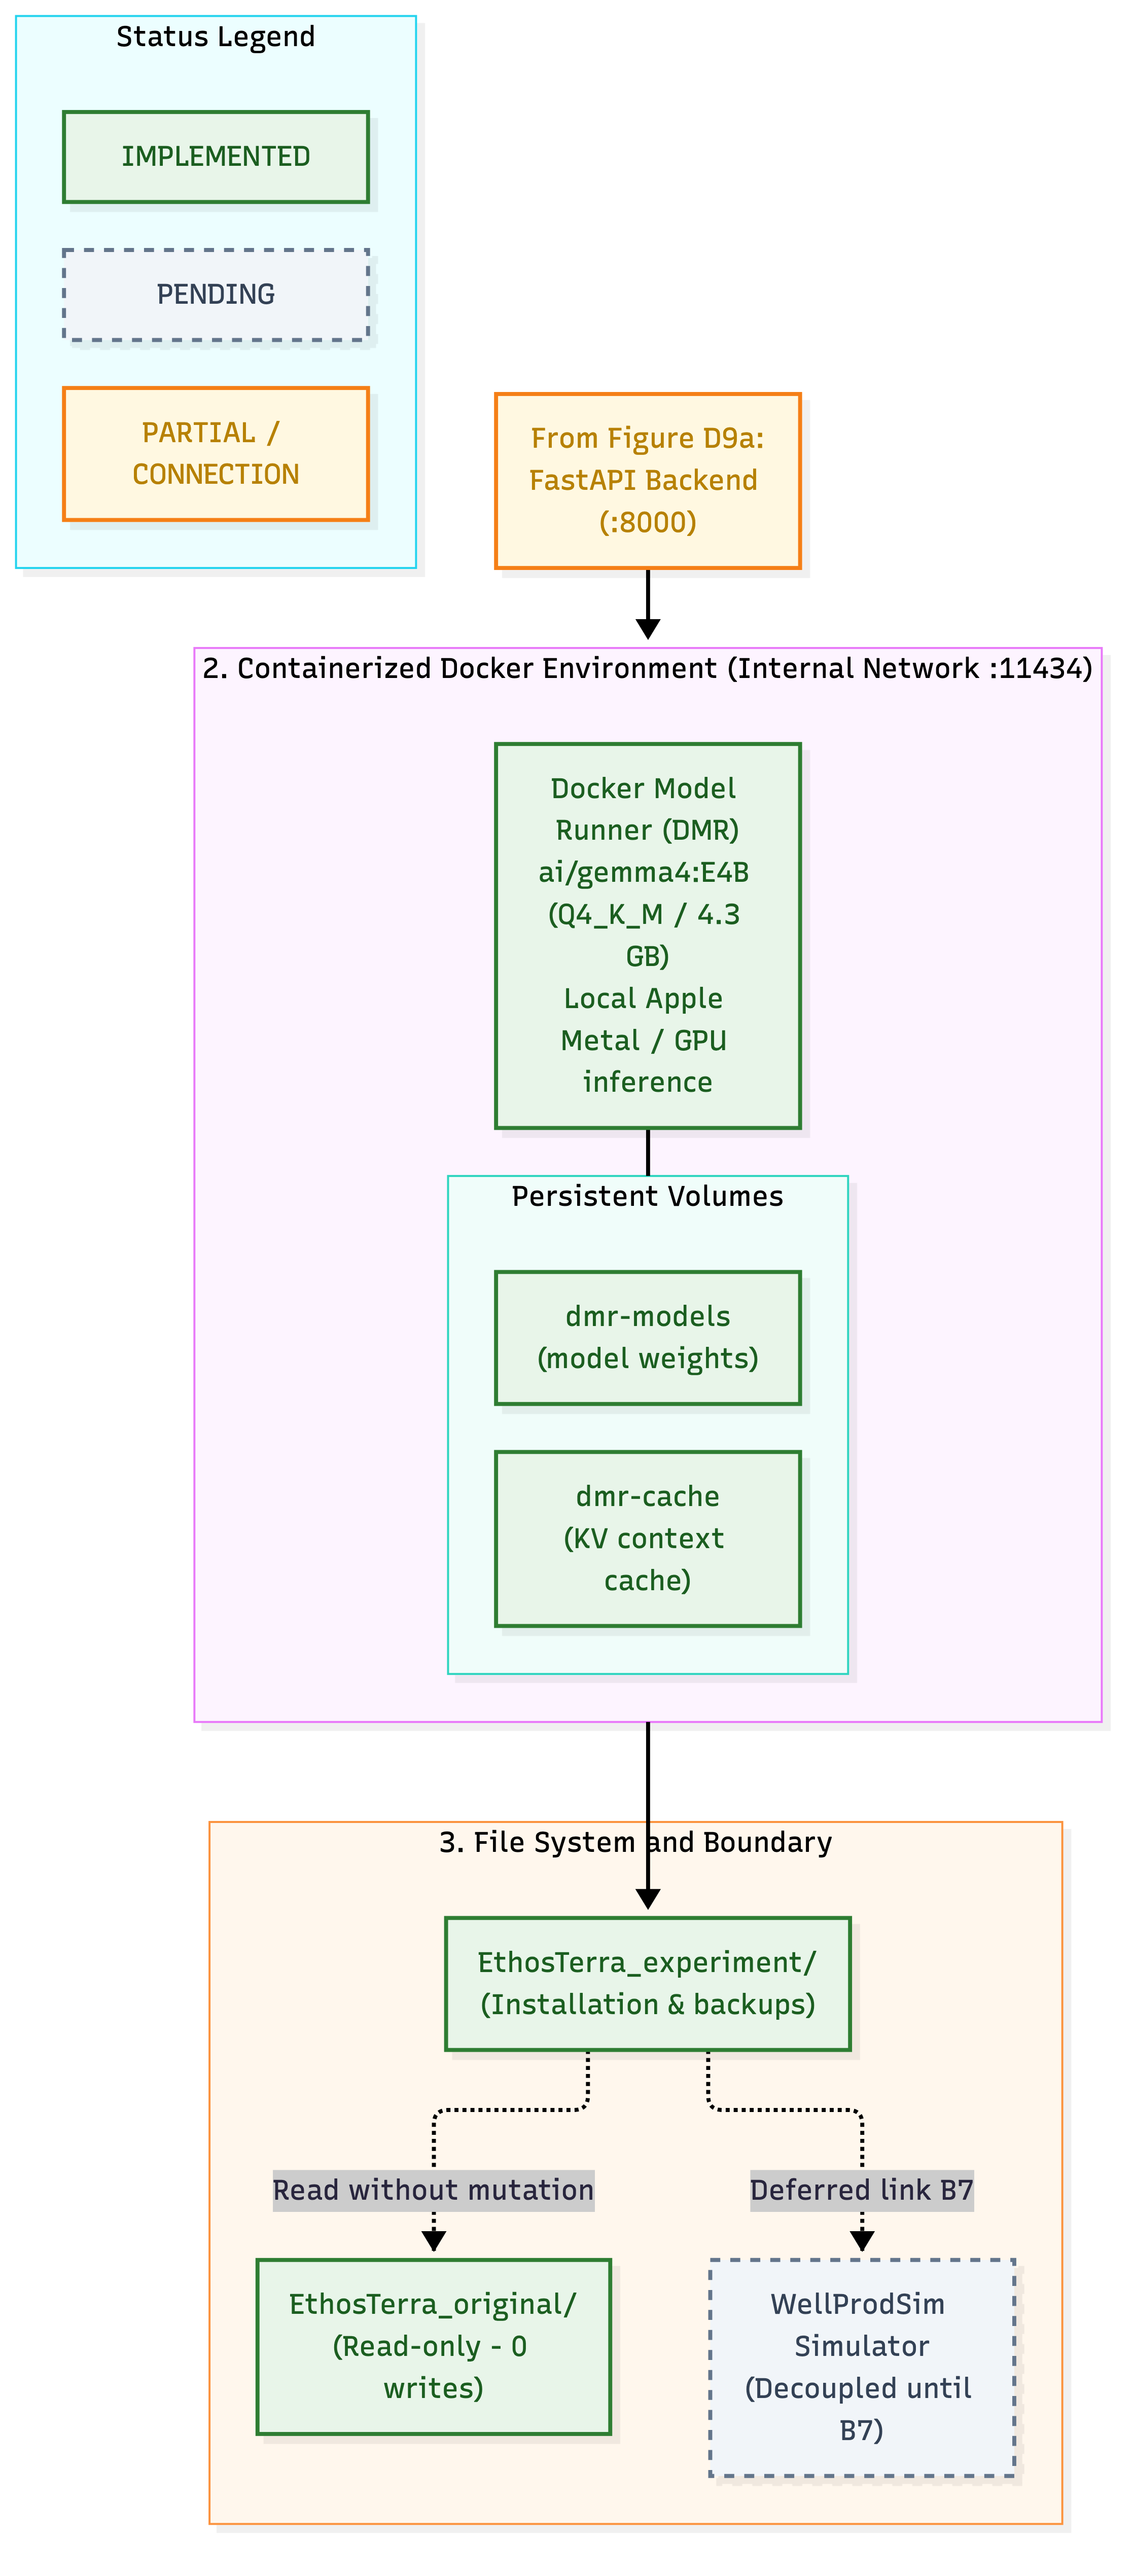
\includegraphics[width=0.88\textwidth,height=0.68\textheight,keepaspectratio]{docs/diagrams/out/d09b_deployment_env_en.png}
    \caption{Figure D9b. Deployment and Execution Environment (Part 2: DMR Containerization and Hardware Resources). Details unified memory allocation on MacBook Air M4 (16~GB), Docker Model Runner container, offline loading of \texttt{ai/gemma4:E4B}, and caveat regarding the 24~GB GPU server reserved for large-scale experimentation.}
    \label{fig:d09b_deployment_env_en}
\end{figure}

% --- Figure D10: Artifact and Evidence Traceability ---
\begin{figure}[htbp]
    \centering
    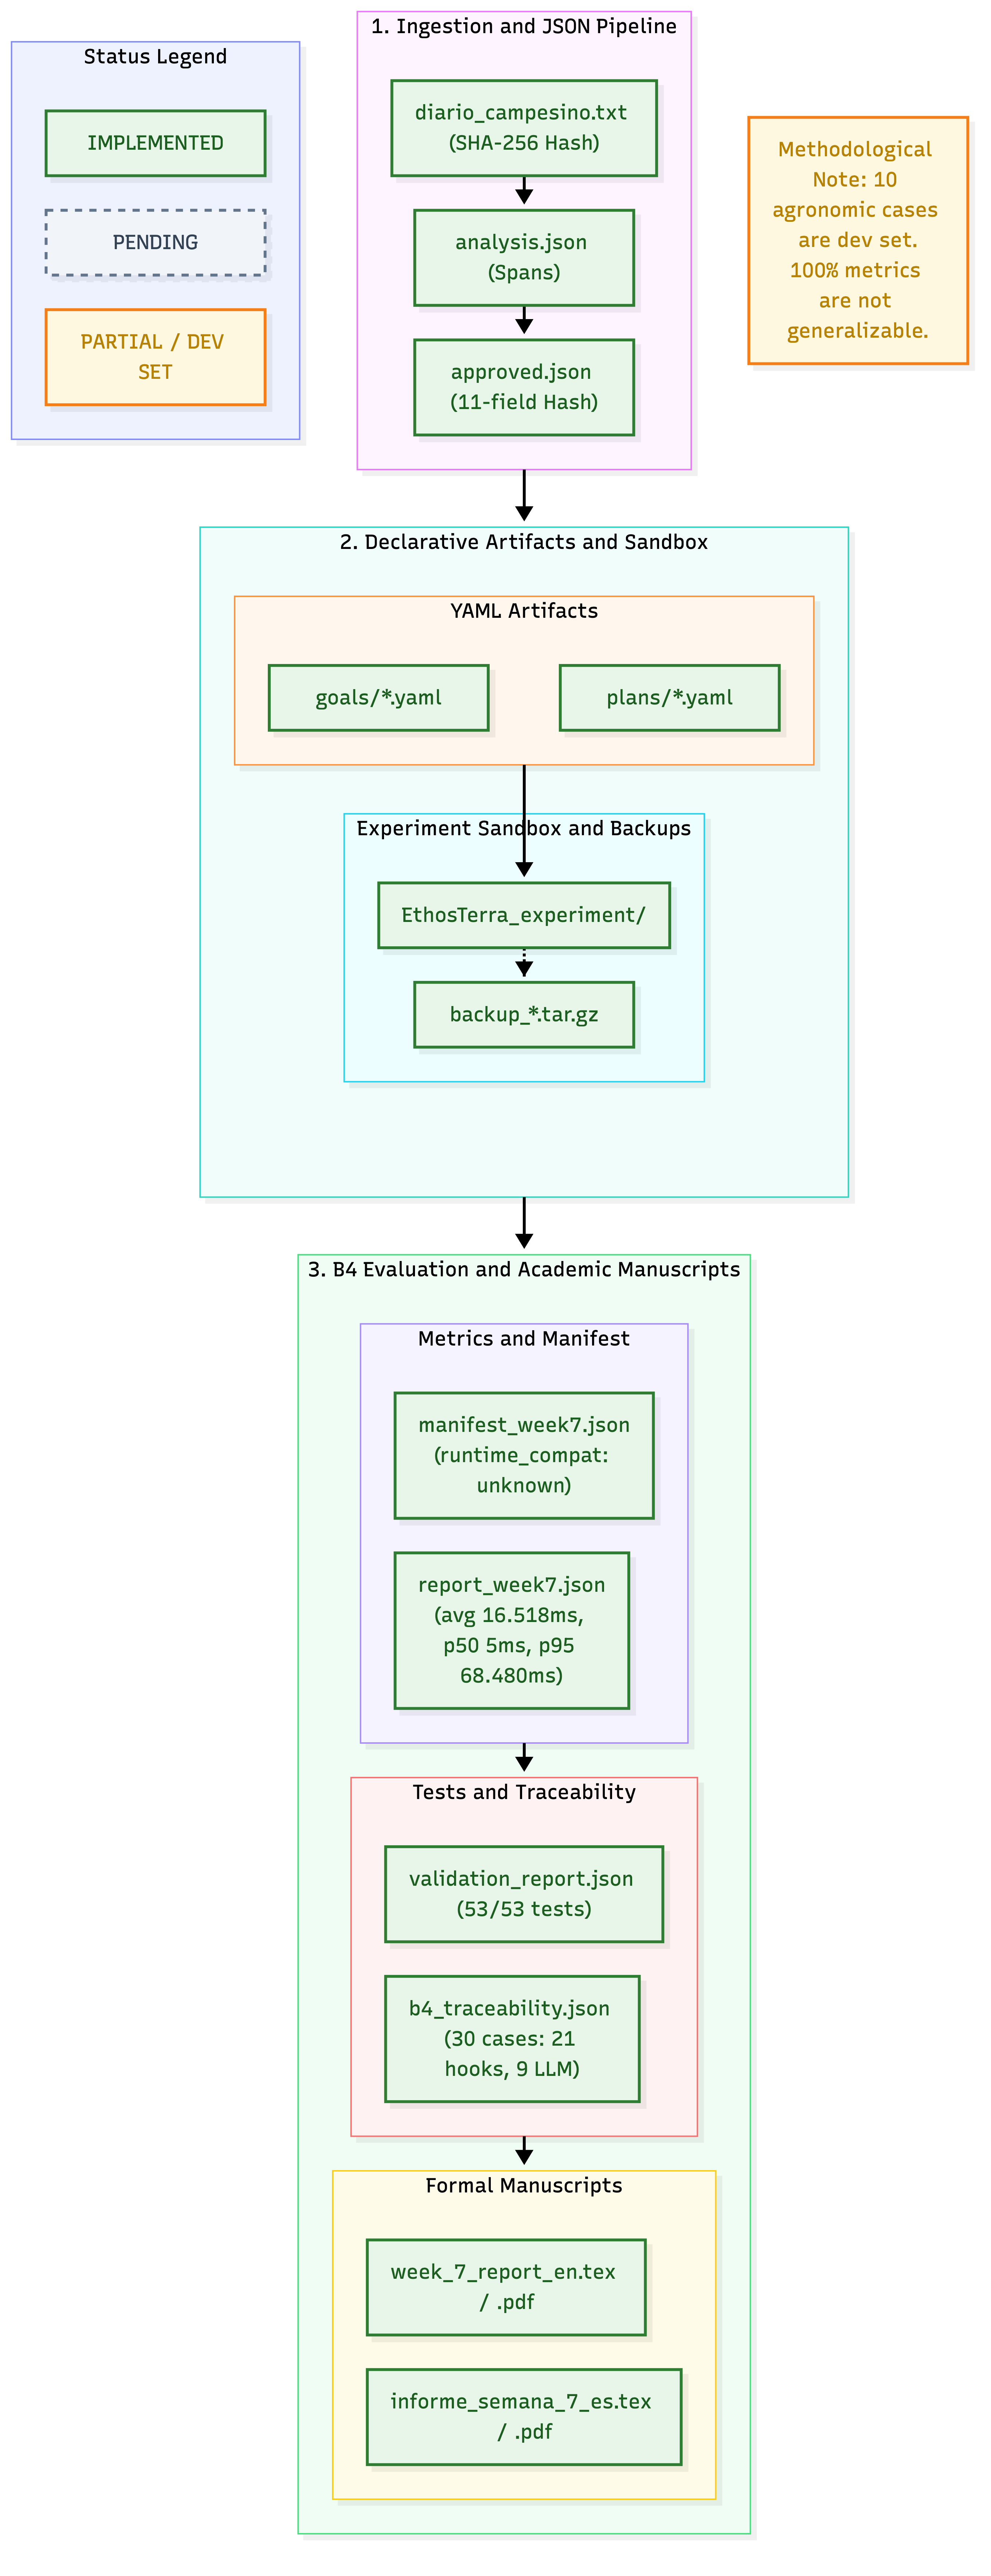
\includegraphics[width=0.88\textwidth,height=0.68\textheight,keepaspectratio]{docs/diagrams/out/d10_artifact_traceability_en.png}
    \caption{Figure D10. Forensic Traceability of Artifacts, Evidence and Reports. Traces the complete chain of custody from field documentary text to academic LaTeX manuscripts, through analysis and approved JSON schemas, generated YAML files, sandbox backups, and evaluation manifests (\texttt{manifest\_week7.json}, \texttt{report\_week7.json}).}
    \label{fig:d10_artifact_traceability_en}
\end{figure}

% --- Figure D12: Boundary View for B5 ---
\begin{figure}[htbp]
    \centering
    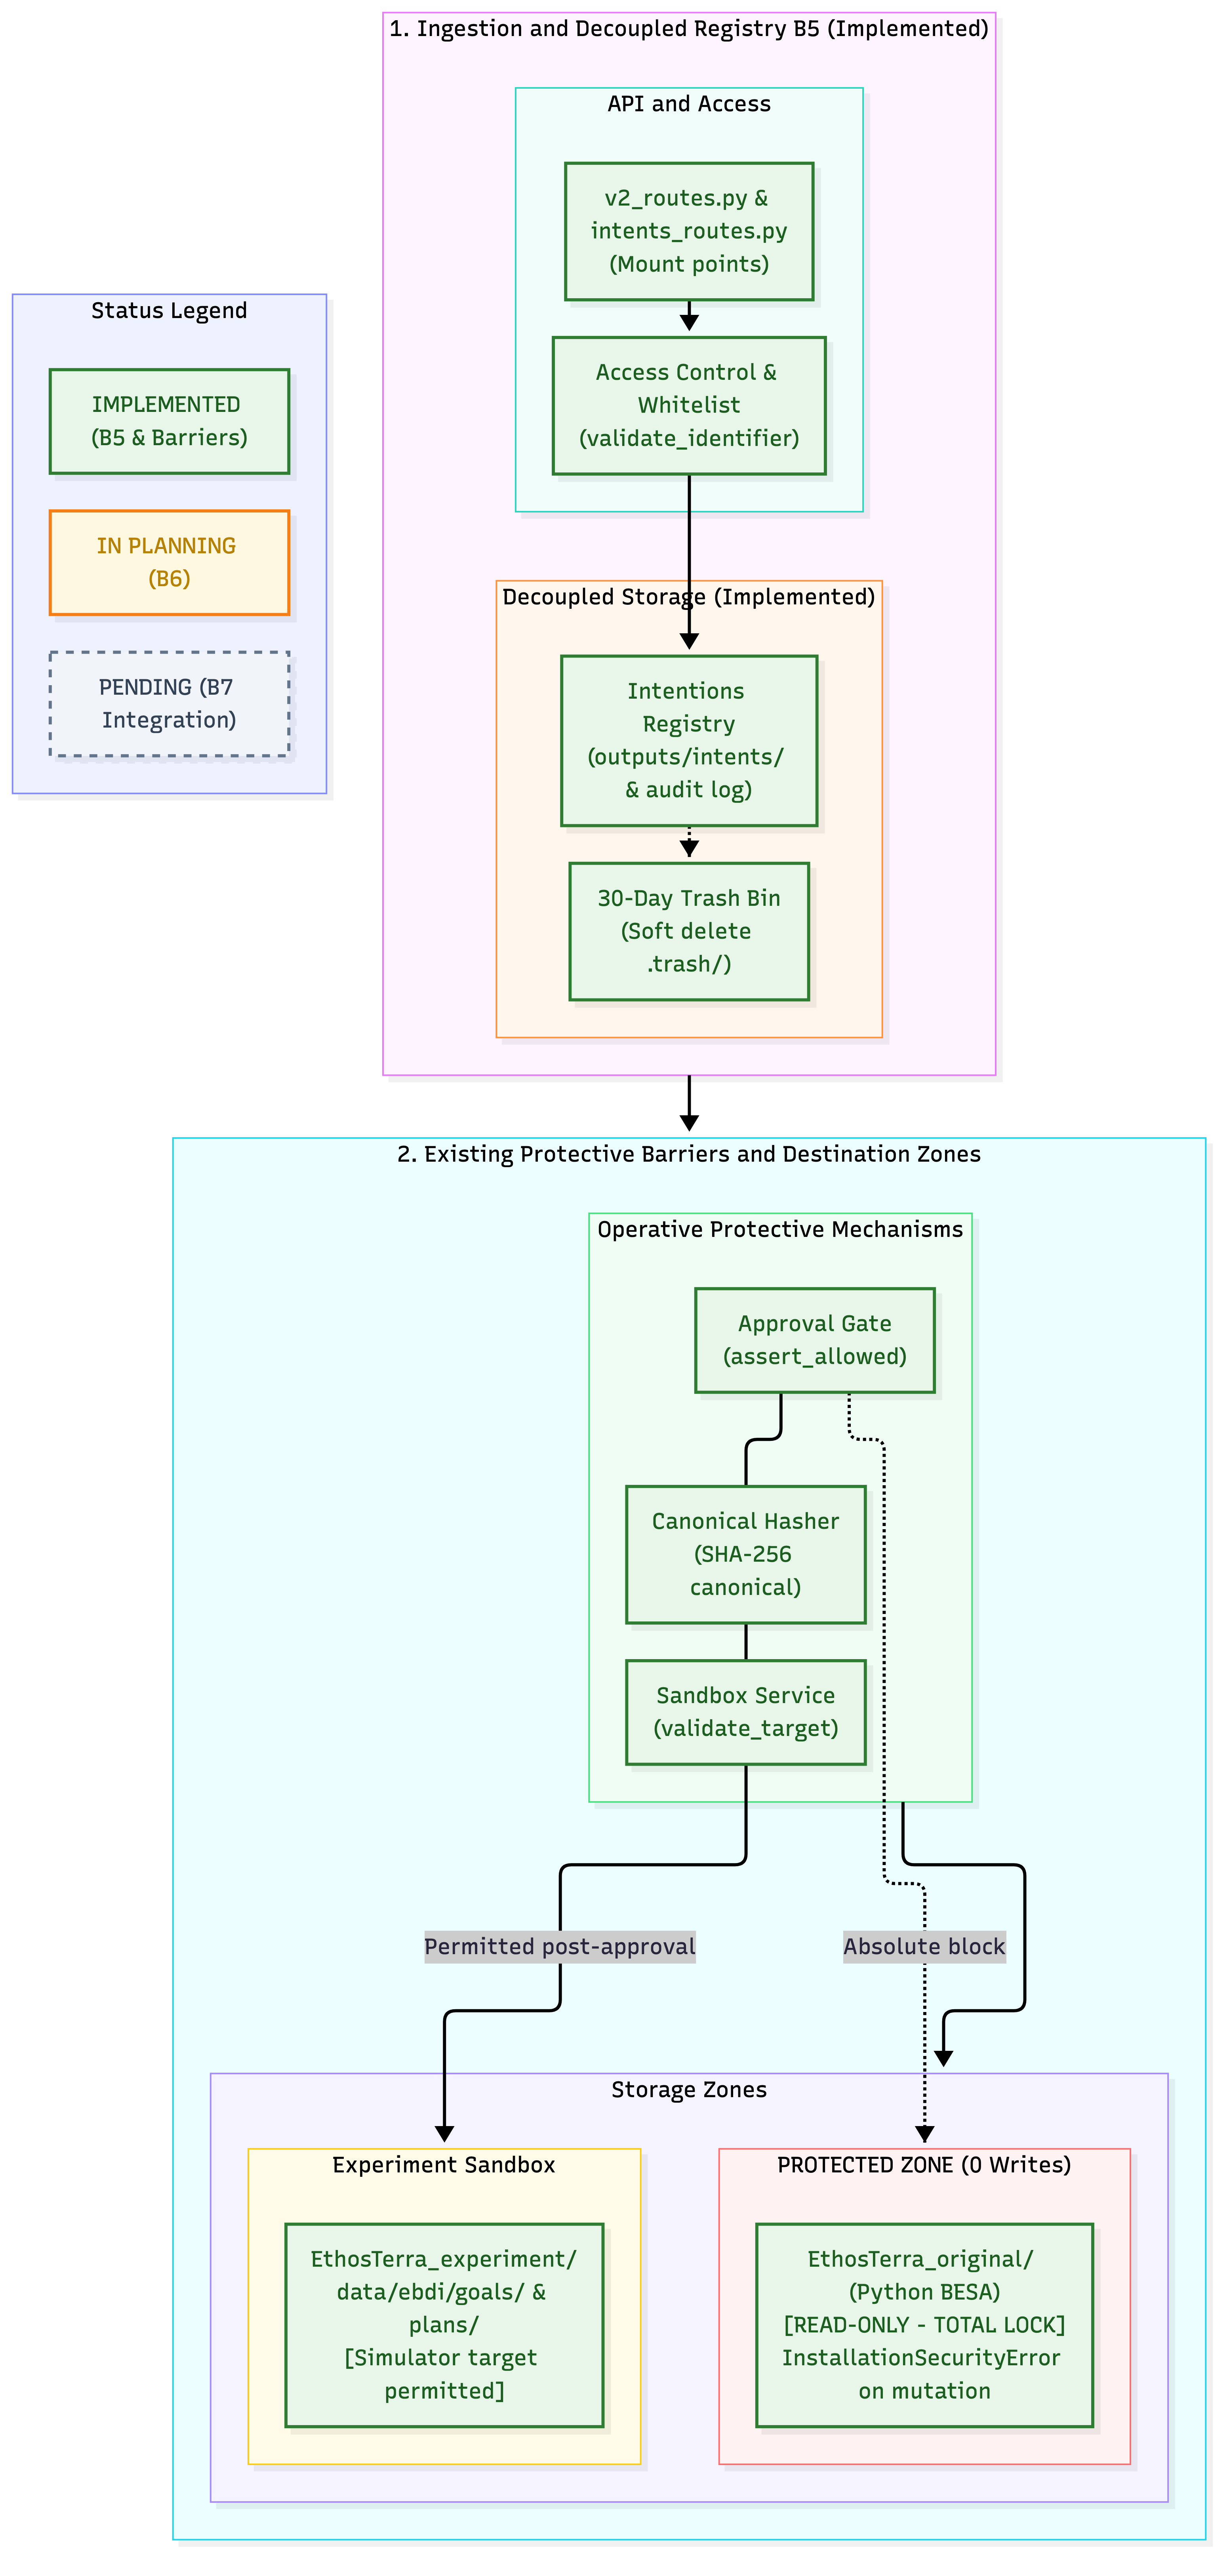
\includegraphics[width=0.88\textwidth,height=0.68\textheight,keepaspectratio]{docs/diagrams/out/d12_b5_boundary_en.png}
    \caption{Figure D12. Architectural Boundary for B5 (Intentions Manual CRUD). The decoupled intentions registry in \texttt{outputs/intents/} and the 30-day soft-delete trash bin are IMPLEMENTED as an autonomous subsystem with whitelist access control and atomic writes. Operative barriers (\texttt{Approval Gate}, \texttt{validate\_target\_sandbox}, and read-only \texttt{EthosTerra\_original/}) remain strictly enforced to preserve the zero-writes-to-core invariant.}
    \label{fig:d12_b5_boundary_en}
\end{figure}
